\documentclass[11pt,fleqn]{book} % Default font size and left-justified equations

\usepackage[top=3cm,bottom=3cm,left=3.2cm,right=3.2cm,headsep=10pt,letterpaper]{geometry} % Page margins

\usepackage{xcolor} % Required for specifying colors by name
% The main color for the document --> Not really ocre.
\definecolor{ocre}{RGB}{215,30,47} % Define the orange color used for highlighting throughout the book
\definecolor{white}{RGB}{255,255,255} 

% Font Settings
\usepackage{avant} % Use the Avantgarde font for headings
%\usepackage{times} % Use the Times font for headings
\usepackage{mathptmx} % Use the Adobe Times Roman as the default text font together with math symbols from the Sym­bol, Chancery and Com­puter Modern fonts

\raggedbottom

\usepackage{microtype} % Slightly tweak font spacing for aesthetics
\usepackage[utf8]{inputenc} % Required for including letters with accents
\usepackage[T1]{fontenc} % Use 8-bit encoding that has 256 glyphs

% %More special packages to help deal with long requirements tables 
% %that might span multiple pages.
\usepackage{multirow} %deal with merged cells in tables
\usepackage{supertabular}
\usepackage{longtable}
\usepackage{morefloats}

\usepackage{url}  \urlstyle{same}     % deal with url strings in bibliography

\usepackage{eurosym}
\usepackage{csquotes}

\usepackage[colorinlistoftodos,prependcaption,textsize=tiny]{todonotes}

% Bibliography
\usepackage[style=numeric,sorting=nyt,sortcites=true,autopunct=true,autolang=hyphen,hyperref=true,abbreviate=false,backref=true,backend=biber]{biblatex}
\addbibresource{me310reportfall.bib} % BibTeX bibliography file
\defbibheading{bibempty}{}

% \usepackage[pdftex,           %Hyperlink cross references, URLs, etc.
%     pdfsubject={ME310 Documentation},
%     colorlinks={true},
%     linkcolor={black},
%     citecolor={blue},
%     bookmarksopenlevel=1,
% ]{hyperref}

\usepackage{me310}

\newcommand{\interviewCitation}[3]{
\begingroup
\vspace{1.2\baselineskip}
\parbox{14.5cm}{\setlength\topsep{0pt}
	\leftskip2em
    \textit{"#1"}\\
    \textit{"#2"}
    \vspace{.5\baselineskip}
    \begin{flushright}
         - \small #3
    \end{flushright}            
}
\vspace{1.0\baselineskip}
\endgroup
}

\newcommand{\fakechaptermark}[1]{\markboth{\normalsize\ #1}{}}

\newcommand{\hiddensection}[1]{
    \stepcounter{section}
    \subsection*{\textcolor{ocre}{\Alph{section}}\hspace{1em}{#1}}
}

\newcommand{\hiddensubsection}[1]{
    \stepcounter{subsection}
    \subsection*{\hspace{-2.5em}\textcolor{ocre}{\Alph{section}.\arabic{subsection}}\hspace{1em}{#1}}
}

\newcommand{\hiddensubsubsection}[1]{
    \stepcounter{subsubsection}
    \subsection*{\hspace{-3.4em}\textcolor{ocre}{\Alph{section}.\arabic{subsection}.\arabic{subsubsection}}\hspace{1em}{#1}}
}

\usepackage{pdfpages}

\usepackage{lettrine}

\usepackage{listings} % for code listings

\usepackage{minted} % for syntax highlighting

%----------------------------------------------------------------------------------------
%	VARIOUS REQUIRED PACKAGES
%----------------------------------------------------------------------------------------

\usepackage{titlesec} % Allows customization of titles

\usepackage{graphicx} % Required for including pictures
\graphicspath{{Figures/}} % Specifies the directory where pictures are stored

\usepackage{lipsum} % Inserts dummy text

\usepackage{tikz} % Required for drawing custom shapes

\usepackage[english]{babel} % English language/hyphenation

\usepackage{enumitem} % Customize lists
\setlist{nolistsep} % Reduce spacing between bullet points and numbered lists

\usepackage{booktabs} % Required for nicer horizontal rules in tables

\usepackage{eso-pic} % Required for specifying an image background in the title page

%----------------------------------------------------------------------------------------
%	MAIN TABLE OF CONTENTS
%----------------------------------------------------------------------------------------

\usepackage{titletoc} % Required for manipulating the table of contents

\contentsmargin{0cm} % Removes the default margin
% Chapter text styling
\titlecontents{chapter}[1.25cm] % Indentation
{\addvspace{15pt}\large\bfseries} % Spacing and font options for chapters
{\color{ocre!60}\contentslabel[\Large\thecontentslabel]{1.25cm}\color{ocre}} % Chapter number
{}  
{\color{ocre!60}\normalsize\bfseries\;\titlerule*[.5pc]{.}\;\thecontentspage} % Page number
% Section text styling
\titlecontents{section}[1.25cm] % Indentation
{\addvspace{5pt}\bfseries} % Spacing and font options for sections
{\contentslabel[\thecontentslabel]{1.25cm}} % Section number
{}
{\hfill\color{black}\thecontentspage} % Page number
[]
% Subsection text styling
\titlecontents{subsection}[1.25cm] % Indentation
{\addvspace{1pt}\small} % Spacing and font options for subsections
{\contentslabel[\thecontentslabel]{1.25cm}} % Subsection number
{}
{\;\titlerule*[.5pc]{.}\;\thecontentspage} % Page number
[] 

%----------------------------------------------------------------------------------------
%	MINI TABLE OF CONTENTS IN CHAPTER HEADS
%----------------------------------------------------------------------------------------

% Section text styling
\titlecontents{lsection}[0em] % Indendating
{\footnotesize\rmfamily} % Font settings
{}
{}
{}

% Subsection text styling
\titlecontents{lsubsection}[.5em] % Indentation
{\normalfont\footnotesize\rmfamily} % Font settings
{}
{}
{}
 
%----------------------------------------------------------------------------------------
%	PAGE HEADERS
%----------------------------------------------------------------------------------------

\usepackage{fancyhdr} % Required for header and footer configuration

\pagestyle{fancy}
\renewcommand{\chaptermark}[1]{\markboth{\rmfamily\normalsize\bfseries\chaptername\ \thechapter.\ #1}{}} % Chapter text font settings
\renewcommand{\sectionmark}[1]{\markright{\rmfamily\normalsize\thesection\hspace{5pt}#1}{}} % Section text font settings
\fancyhf{} \fancyhead[LE,RO]{\rmfamily\normalsize\thepage} % Font setting for the page number in the header
\fancyhead[LO]{\rightmark} % Print the nearest section name on the left side of odd pages
\fancyhead[RE]{\leftmark} % Print the current chapter name on the right side of even pages
\renewcommand{\headrulewidth}{0.5pt} % Width of the rule under the header
\addtolength{\headheight}{2.5pt} % Increase the spacing around the header slightly
\renewcommand{\footrulewidth}{0pt} % Removes the rule in the footer
\fancypagestyle{plain}{\fancyhead{}\renewcommand{\headrulewidth}{0pt}} % Style for when a plain pagestyle is specified

% Removes the header from odd empty pages at the end of chapters
\makeatletter
\renewcommand{\cleardoublepage}{
\clearpage\ifodd\c@page\else
\hbox{}
\vspace*{\fill}
\thispagestyle{empty}
\newpage
\fi}

%----------------------------------------------------------------------------------------
%	THEOREM STYLES
%----------------------------------------------------------------------------------------

\usepackage{amsmath,amsfonts,amssymb,amsthm} % For math equations, theorems, symbols, etc

\newcommand{\intoo}[2]{\mathopen{]}#1\,;#2\mathclose{[}}
\newcommand{\ud}{\mathop{\mathrm{{}d}}\mathopen{}}
\newcommand{\intff}[2]{\mathopen{[}#1\,;#2\mathclose{]}}
\newtheorem{notation}{Notation}[chapter]

%%%%%%%%%%%%%%%%%%%%%%%%%%%%%%%%%%%%%%%%%%%%%%%%%%%%%%%%%%%%%%%%%%%%%%%%%%%
%%%%%%%%%%%%%%%%%%%% dedicated to boxed/framed environements %%%%%%%%%%%%%%
%%%%%%%%%%%%%%%%%%%%%%%%%%%%%%%%%%%%%%%%%%%%%%%%%%%%%%%%%%%%%%%%%%%%%%%%%%%
\newtheoremstyle{ocrenumbox}% % Theorem style name
{0pt}% Space above
{0pt}% Space below
{\normalfont}% % Body font
{}% Indent amount
{\small\bf\color{ocre}}% % Theorem head font
{\;}% Punctuation after theorem head
{0.25em}% Space after theorem head
{\small\color{ocre}\thmname{#1}\nobreakspace\thmnumber{\@ifnotempty{#1}{}\@upn{#2}}% Theorem text (e.g. Theorem 2.1)
\thmnote{\nobreakspace\the\thm@notefont\bfseries\color{black}---\nobreakspace#3.}} % Optional theorem note
\renewcommand{\qedsymbol}{$\blacksquare$}% Optional qed square

\newtheoremstyle{blacknumex}% Theorem style name
{5pt}% Space above
{5pt}% Space below
{\normalfont}% Body font
{} % Indent amount
{\small\bf\sffamily}% Theorem head font
{\;}% Punctuation after theorem head
{0.25em}% Space after theorem head
{\small{\tiny\ensuremath{\blacksquare}}\nobreakspace\thmname{#1}\nobreakspace\thmnumber{\@ifnotempty{#1}{}\@upn{#2}}% Theorem text (e.g. Theorem 2.1)
\thmnote{\nobreakspace\the\thm@notefont\sffamily\bfseries---\nobreakspace#3.}}% Optional theorem note

\newtheoremstyle{blacknumbox} % Theorem style name
{0pt}% Space above
{0pt}% Space below
{\normalfont}% Body font
{}% Indent amount
{\small\bf\sffamily}% Theorem head font
{\;}% Punctuation after theorem head
{0.25em}% Space after theorem head
{\small\sffamily\thmname{#1}\nobreakspace\thmnumber{\@ifnotempty{#1}{}\@upn{#2}}% Theorem text (e.g. Theorem 2.1)
\thmnote{\nobreakspace\the\thm@notefont\sffamily\bfseries---\nobreakspace#3.}}% Optional theorem note

%%%%%%%%%%%%%%%%%%%%%%%%%%%%%%%%%%%%%%%%%%%%%%%%%%%%%%%%%%%%%%%%%%%%%%%%%%%
%%%%%%%%%%%%% dedicated to non-boxed/non-framed environements %%%%%%%%%%%%%
%%%%%%%%%%%%%%%%%%%%%%%%%%%%%%%%%%%%%%%%%%%%%%%%%%%%%%%%%%%%%%%%%%%%%%%%%%%
\newtheoremstyle{ocrenum}% % Theorem style name
{5pt}% Space above
{5pt}% Space below
{\normalfont}% % Body font
{}% Indent amount
{\small\bf\sffamily\color{ocre}}% % Theorem head font
{\;}% Punctuation after theorem head
{0.25em}% Space after theorem head
{\small\sffamily\color{ocre}\thmname{#1}\nobreakspace\thmnumber{\@ifnotempty{#1}{}\@upn{#2}}% Theorem text (e.g. Theorem 2.1)
\thmnote{\nobreakspace\the\thm@notefont\sffamily\bfseries\color{black}---\nobreakspace#3.}} % Optional theorem note
\renewcommand{\qedsymbol}{$\blacksquare$}% Optional qed square
\makeatother

% Defines the theorem text style for each type of theorem to one of the three styles above
\newcounter{dummy} 
\numberwithin{dummy}{section}
\theoremstyle{ocrenumbox}
\newtheorem{theoremeT}[dummy]{Theorem}
\newtheorem{problem}{Problem}[chapter]
\newtheorem{exerciseT}{Exercise}[chapter]
\theoremstyle{blacknumex}
\newtheorem{exampleT}{Example}[chapter]
\theoremstyle{blacknumbox}
\newtheorem{vocabulary}{Vocabulary}[chapter]
\newtheorem{definitionT}{Definition}[section]
\newtheorem{corollaryT}[dummy]{Corollary}
\theoremstyle{ocrenum}
\newtheorem{proposition}[dummy]{Proposition}

%----------------------------------------------------------------------------------------
%	DEFINITION OF COLORED BOXES
%----------------------------------------------------------------------------------------

\RequirePackage[framemethod=default]{mdframed} % Required for creating the theorem, definition, exercise and corollary boxes

% Theorem box
\newmdenv[skipabove=7pt,
skipbelow=7pt,
backgroundcolor=black!5,
linecolor=ocre,
innerleftmargin=5pt,
innerrightmargin=5pt,
innertopmargin=5pt,
leftmargin=0cm,
rightmargin=0cm,
innerbottommargin=5pt]{tBox}

% Exercise box	  
\newmdenv[skipabove=7pt,
skipbelow=7pt,
rightline=false,
leftline=true,
topline=false,
bottomline=false,
backgroundcolor=ocre!10,
linecolor=ocre,
innerleftmargin=5pt,
innerrightmargin=5pt,
innertopmargin=5pt,
innerbottommargin=5pt,
leftmargin=0cm,
rightmargin=0cm,
linewidth=4pt]{eBox}	

% Definition box
\newmdenv[skipabove=7pt,
skipbelow=7pt,
rightline=false,
leftline=true,
topline=false,
bottomline=false,
linecolor=ocre,
innerleftmargin=5pt,
innerrightmargin=5pt,
innertopmargin=0pt,
leftmargin=0cm,
rightmargin=0cm,
linewidth=4pt,
innerbottommargin=0pt]{dBox}	

% Corollary box
\newmdenv[skipabove=7pt,
skipbelow=7pt,
rightline=false,
leftline=true,
topline=false,
bottomline=false,
linecolor=gray,
backgroundcolor=black!5,
innerleftmargin=5pt,
innerrightmargin=5pt,
innertopmargin=5pt,
leftmargin=0cm,
rightmargin=0cm,
linewidth=4pt,
innerbottommargin=5pt]{cBox}

% Creates an environment for each type of theorem and assigns it a theorem text style from the "Theorem Styles" section above and a colored box from above
\newenvironment{theorem}{\begin{tBox}\begin{theoremeT}}{\end{theoremeT}\end{tBox}}
\newenvironment{exercise}{\begin{eBox}\begin{exerciseT}}{\hfill{\color{ocre}\tiny\ensuremath{\blacksquare}}\end{exerciseT}\end{eBox}}				  
\newenvironment{definition}{\begin{dBox}\begin{definitionT}}{\end{definitionT}\end{dBox}}	
\newenvironment{example}{\begin{exampleT}}{\hfill{\tiny\ensuremath{\blacksquare}}\end{exampleT}}		
\newenvironment{corollary}{\begin{cBox}\begin{corollaryT}}{\end{corollaryT}\end{cBox}}	

%----------------------------------------------------------------------------------------
%	REMARK ENVIRONMENT
%----------------------------------------------------------------------------------------

\newenvironment{remark}{\par\vspace{10pt}\small % Vertical white space above the remark and smaller font size
\begin{list}{}{
\leftmargin=35pt % Indentation on the left
\rightmargin=25pt}\item\ignorespaces % Indentation on the right
\makebox[-2.5pt]{\begin{tikzpicture}[overlay]
\node[draw=ocre!60,line width=1pt,circle,fill=ocre!25,font=\sffamily\bfseries,inner sep=2pt,outer sep=0pt] at (-15pt,0pt){\textcolor{ocre}{R}};\end{tikzpicture}} % Orange R in a circle
\advance\baselineskip -1pt}{\end{list}\vskip5pt} % Tighter line spacing and white space after remark

%----------------------------------------------------------------------------------------
%	SECTION NUMBERING IN THE MARGIN
%----------------------------------------------------------------------------------------

\makeatletter
\renewcommand{\@seccntformat}[1]{\llap{\textcolor{ocre}{\csname the#1\endcsname}\hspace{1em}}}                    
\renewcommand{\section}{\@startsection{section}{1}{\z@}
{-4ex \@plus -1ex \@minus -.4ex}
{1ex \@plus.2ex }
{\normalfont\large\bfseries}}
\renewcommand{\subsection}{\@startsection {subsection}{2}{\z@}
{-3ex \@plus -0.1ex \@minus -.4ex}
{0.5ex \@plus.2ex }
{\normalfont\bfseries}}
\renewcommand{\subsubsection}{\@startsection {subsubsection}{3}{\z@}
{-2ex \@plus -0.1ex \@minus -.2ex}
{.2ex \@plus.2ex }
{\normalfont\small\bfseries\itshape}}                        
\renewcommand\paragraph{\@startsection{paragraph}{4}{\z@}
{-2ex \@plus-.2ex \@minus .2ex}
{.1ex}
{\normalfont\small\bfseries}}

%----------------------------------------------------------------------------------------
%	HYPERLINKS IN THE DOCUMENTS
%----------------------------------------------------------------------------------------

% For an unclear reason, the package should be loaded now and not later
\usepackage{hyperref}
\hypersetup{hidelinks,colorlinks=false,breaklinks=true,urlcolor= ocre,bookmarksopen=false,pdftitle={Title},pdfauthor={Author}}

%----------------------------------------------------------------------------------------
%	CHAPTER HEADINGS
%----------------------------------------------------------------------------------------

% The set-up below should be (sadly) manually adapted to the overall margin page septup controlled by the geometry package loaded in the main.tex document. It is possible to implement below the dimensions used in the goemetry package (top,bottom,left,right)... TO BE DONE

\newcommand{\thechapterimage}{}
\newcommand{\chapterimage}[1]{\renewcommand{\thechapterimage}{#1}}

% Numbered chapters with mini tableofcontents
\def\thechapter{\arabic{chapter}}
\def\@makechapterhead#1{
\thispagestyle{empty}
{\centering \normalfont\rmfamily
\ifnum \c@secnumdepth >\m@ne
\if@mainmatter
\startcontents
\begin{tikzpicture}[remember picture,overlay]
\node at (current page.north west)
{\begin{tikzpicture}[remember picture,overlay]
\node[anchor=north west,inner sep=0pt] at (0,0) {\includegraphics[width=\paperwidth]{\thechapterimage}};
%%%%%%%%%%%%%%%%%%%%%%%%%%%%%%%%%%%%%%%%%%%%%%%%%%%%%%%%%%%%%%%%%%%%%%%%%%%%%%%%%%%%%
% Commenting the 3 lines below removes the small contents box in the chapter heading
%\fill[color=ocre!10!white,opacity=.6] (1cm,0) rectangle (8cm,-7cm);
%\node[anchor=north west] at (1.1cm,.35cm) {\parbox[t][8cm][t]{6.5cm}{\huge\bfseries\flushleft \printcontents{l}{1}{\setcounter{tocdepth}{2}}}};
\draw[anchor=west] (5cm,-9cm) node [rounded corners=20pt,fill=ocre!10!white,text opacity=1,draw=ocre,draw opacity=1,line width=1.5pt,fill opacity=.6,inner sep=12pt]{\huge\rmfamily\bfseries\textcolor{black}{\thechapter. #1\strut\makebox[22cm]{}}};
%%%%%%%%%%%%%%%%%%%%%%%%%%%%%%%%%%%%%%%%%%%%%%%%%%%%%%%%%%%%%%%%%%%%%%%%%%%%%%%%%%%%%
\end{tikzpicture}};
\end{tikzpicture}}
\par\vspace*{230\p@}
\fi
\fi}

% Unnumbered chapters without mini tableofcontents (could be added though) 
\def\@makeschapterhead#1{
\thispagestyle{empty}
{\centering \normalfont\sffamily
\ifnum \c@secnumdepth >\m@ne
\if@mainmatter
\begin{tikzpicture}[remember picture,overlay]
\node at (current page.north west)
{\begin{tikzpicture}[remember picture,overlay]
\node[anchor=north west,inner sep=0pt] at (0,0) {\includegraphics[width=\paperwidth]{\thechapterimage}};
\draw[anchor=west] (5cm,-9cm) node [rounded corners=20pt,fill=ocre!10!white,fill opacity=.6,inner sep=12pt,text opacity=1,draw=ocre,draw opacity=1,line width=1.5pt]{\huge\sffamily\bfseries\textcolor{black}{#1\strut\makebox[22cm]{}}};
\end{tikzpicture}};
\end{tikzpicture}}
\par\vspace*{230\p@}
\fi
\fi
}
\makeatother % Insert the commands.tex file which contains the majority of the structure behind the template

\begin{document}


%%%%%%%%%% TITLE PAGE%%%%%%%%%%%%%%%%

\thispagestyle{empty}
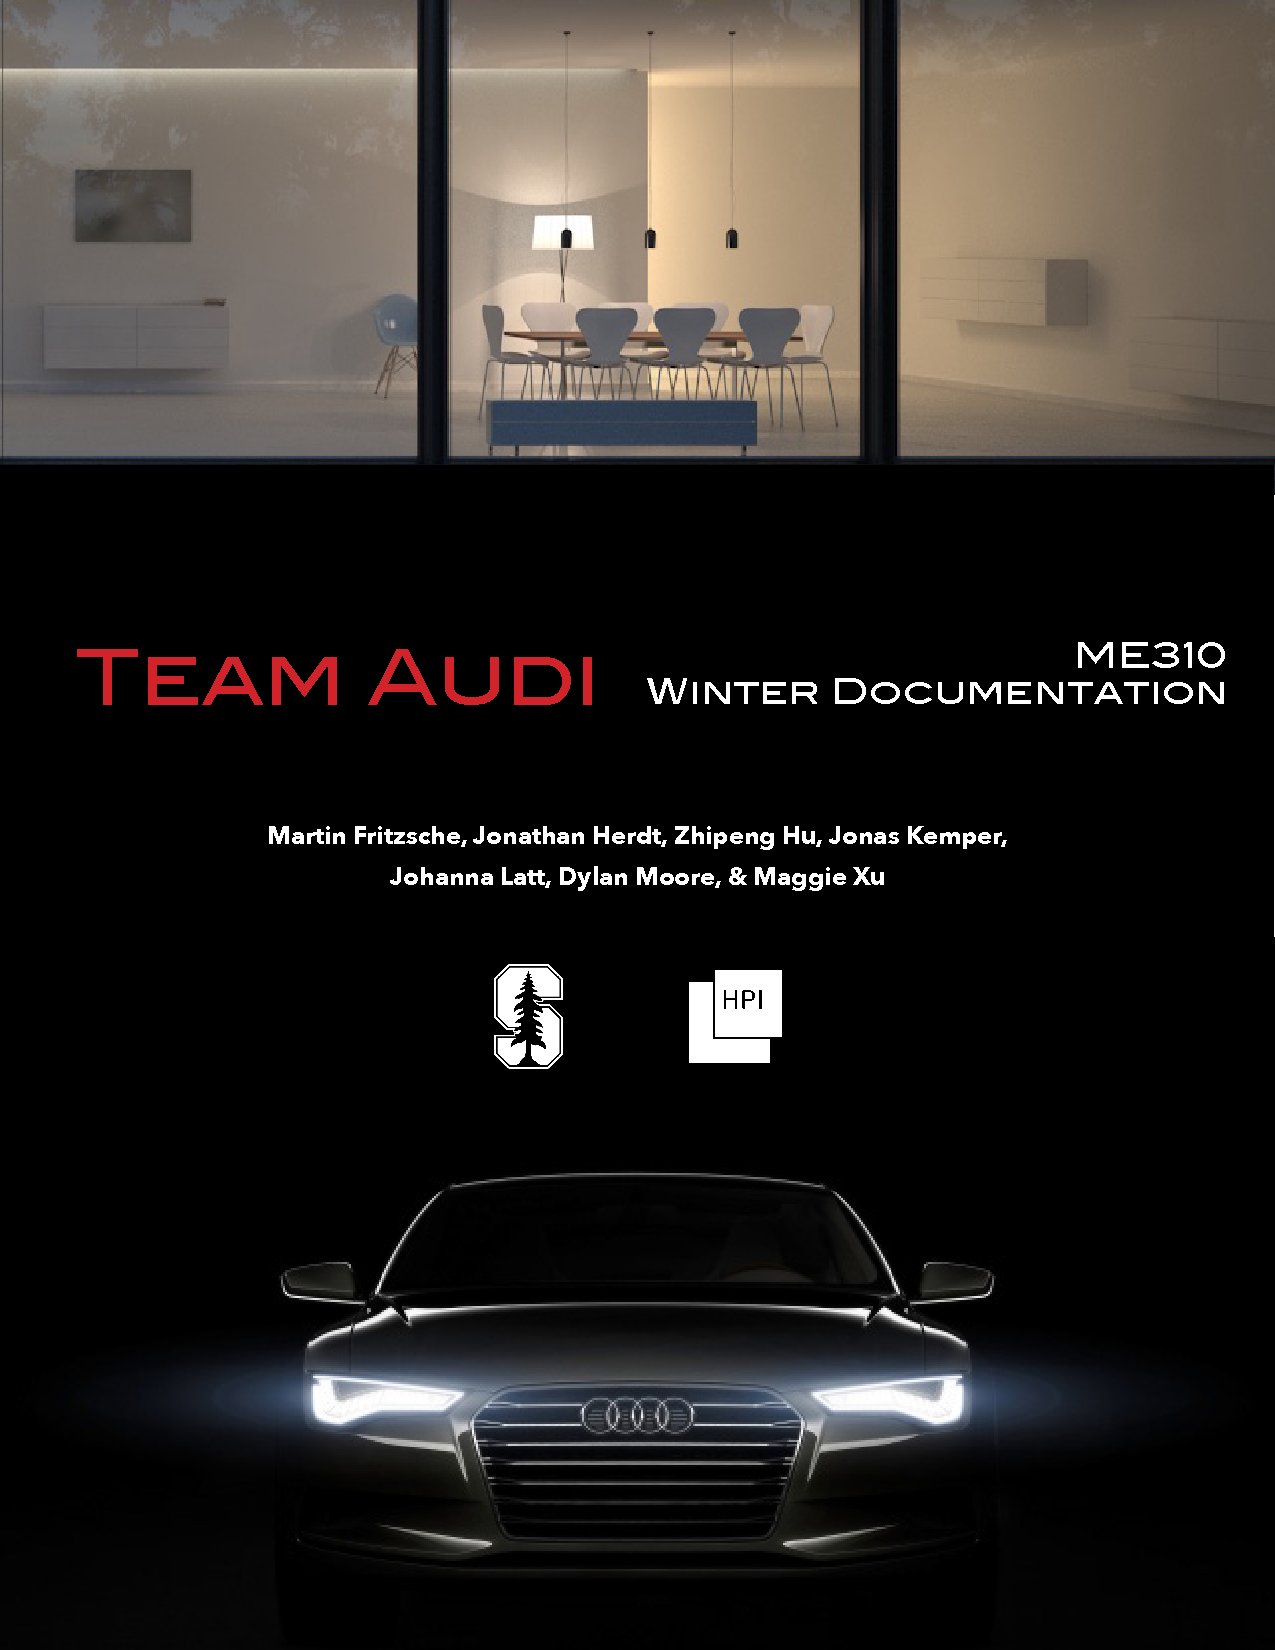
\includepdf[pages={1}]{00_cover_page.pdf}

%%%%%%%%%BEGIN ANY CUSTOM ABBREVIATIONS%%%%%%
% Define any abbreviations that will apply throughout the document
% to save typing. Examples:
%\def\pmt{{\em Papier M\^{a}ch\`{e}}}  %Define "\pmt" to print "Papier Mache" with accents +1space
%\def\cbike{{\em Casterbike} \,}  %Define "\cbike" to print "Casterbike " italicized +1space
%%%%%%%%%END CUSTOM ABBREVIATIONS%%%%%%%%%

%%%%%%%%COMMENTS%%%%%%%%%%%%%%%%
%Allow comments ('remarks') to be shown or hidden.
% Put optional text in \begin{remark} ... \end{remark}  environments.
%The usage is a bit counterintuitive: \commentsoff makes them visible; \commentson hides them.
%\commentson{remark} %Don't print remarks.
%\commentsoff{remark}  %Do print remarks. 


%%%%%%%%%%%%%%%%%%%%%%%%%%%%%%%%%%%%%%%%
%   BEGIN THE MAIN DOCUMENT
%%%%%%%%%%%%%%%%%%%%%%%%%%%%%%%%%%%%%%%%

%%%%%%%%%%%%%%%%%%%%%%%%
% Load file "Executive.tex" for the Executive summary.
% Remember, this is a stand-alone section for executives to read.
%The executive summary is a special chapter before the TOC
% See the other sections (e.g. Context) for more normal chapter headings
%%%%%%%%%%%%%%%%%%%%%%%%%%%%%%%%%%%%
\todo{Call it Front Matter in TOC, as it will include Glossary and auto-generated TOC, LOF.}
\chapterimage{ChapterImages/teaser} % Chapter heading image
\chapter[Front Matter]{Executive Summary} 
\label{cha:front}
%\addcontentsline{toc}{section}{Executive Summary}
%%%%%%%%%%%%%%%%%%%%%%%%%%%%%%%%%%%%
%Begin the actual executive summary text. If you create any subsections you
%probably want to use  \section*{Section name}  with an asterisk, so they are not numbered.
% Note: to get proper looking quotes use two left/right single quotes: ``. . . ''

%%%%%%Example of a remark that can optionally be printed:
% \begin{remark}\color{blue}
% \emph{(To hide these blue remarks, set} \verb'commentson' \emph{in AUDI\_FallDoc.tex)}

% Suggested length of this section: 2-2.5 pages including figure(s).
% \noindent This the most important section to edit carefully. It should stand alone. Assume it is the \emph{only} section that your
% corporate liaison's boss will read.
% \begin{itemize} %\tightlist   % a list with reduced white space
% \item Introduce the reader to what your project is about. 
% \item You can use your Fall Brochure as a starting point.
% \item Say something brief to introduce the design team (local + global).
% \item Motivate the current project direction (based on findings from users and experts,
% benchmarking, CEP or CFP, etc.).
% \item What you did is less important than \textbf{what you learned}.  What findings or insights do you have?
% \item Make sure your current ``Point of View'' comes across. The person who reads only the Executive
% Summary should still have an idea who your User is.
% \item Include images that capture the gist of your design problem and vision.
% If an image from your CFP, CEP is helpful, use it! Because this is a stand-alone section, it's fine
% to duplicate any images from this section elsewhere in the main document.
% \end{itemize}

% The remainder of this section is taken from 
% %\cite{Autodesk2008Fall}
% , a pretty good Fall document, done in Latex.
% \normalcolor
% \end{remark}
% %%%%End of remark


%%%%%%%%%%%%%%%%%%BEGIN EXAMPLE TEXT FOR THIS SECTION %%%%%%%%%%%%
\lettrine[lines=2]{W}{\ \ hat} are people most concerned with during their transition between home and being on their way? When leaving their home and upon arriving, people have a set list of things to keep in mind: ``Did I pack everything I will need for the day?'' is one crucial aspect that becomes most pressing before leaving, while ``How can I quickly disarm my alarm system and make sure I don't forget about it?'' becomes relevant upon return. Our set goal is to make this transition easier for Audi customers, to support them in what they already do, to remind them of things they forgot and to put them in control of what happens when.
% We therefore propose two different systems that both take a smart home and a smart car as given circumstances. We strongly believe that the coming 3 to 5 years will bring more interconnectedness, making available open connections to a variety of smart devices such as alarm systems, window and door sensors, as well as data around the car's status.

To make this possible, we propose a device we call AudiSeamless. It addresses two main concerns users have around their departure from and arrival to their home. 
\begin{enumerate}
    \item Upon \textbf{departure,} helps users remember about things they need to take care of before leaving.
    \item Upon \textbf{arrival,} helps users to disarm their alarm system in a secure and user-friendly way.
\end{enumerate}


\begin{figure}
  \centering
    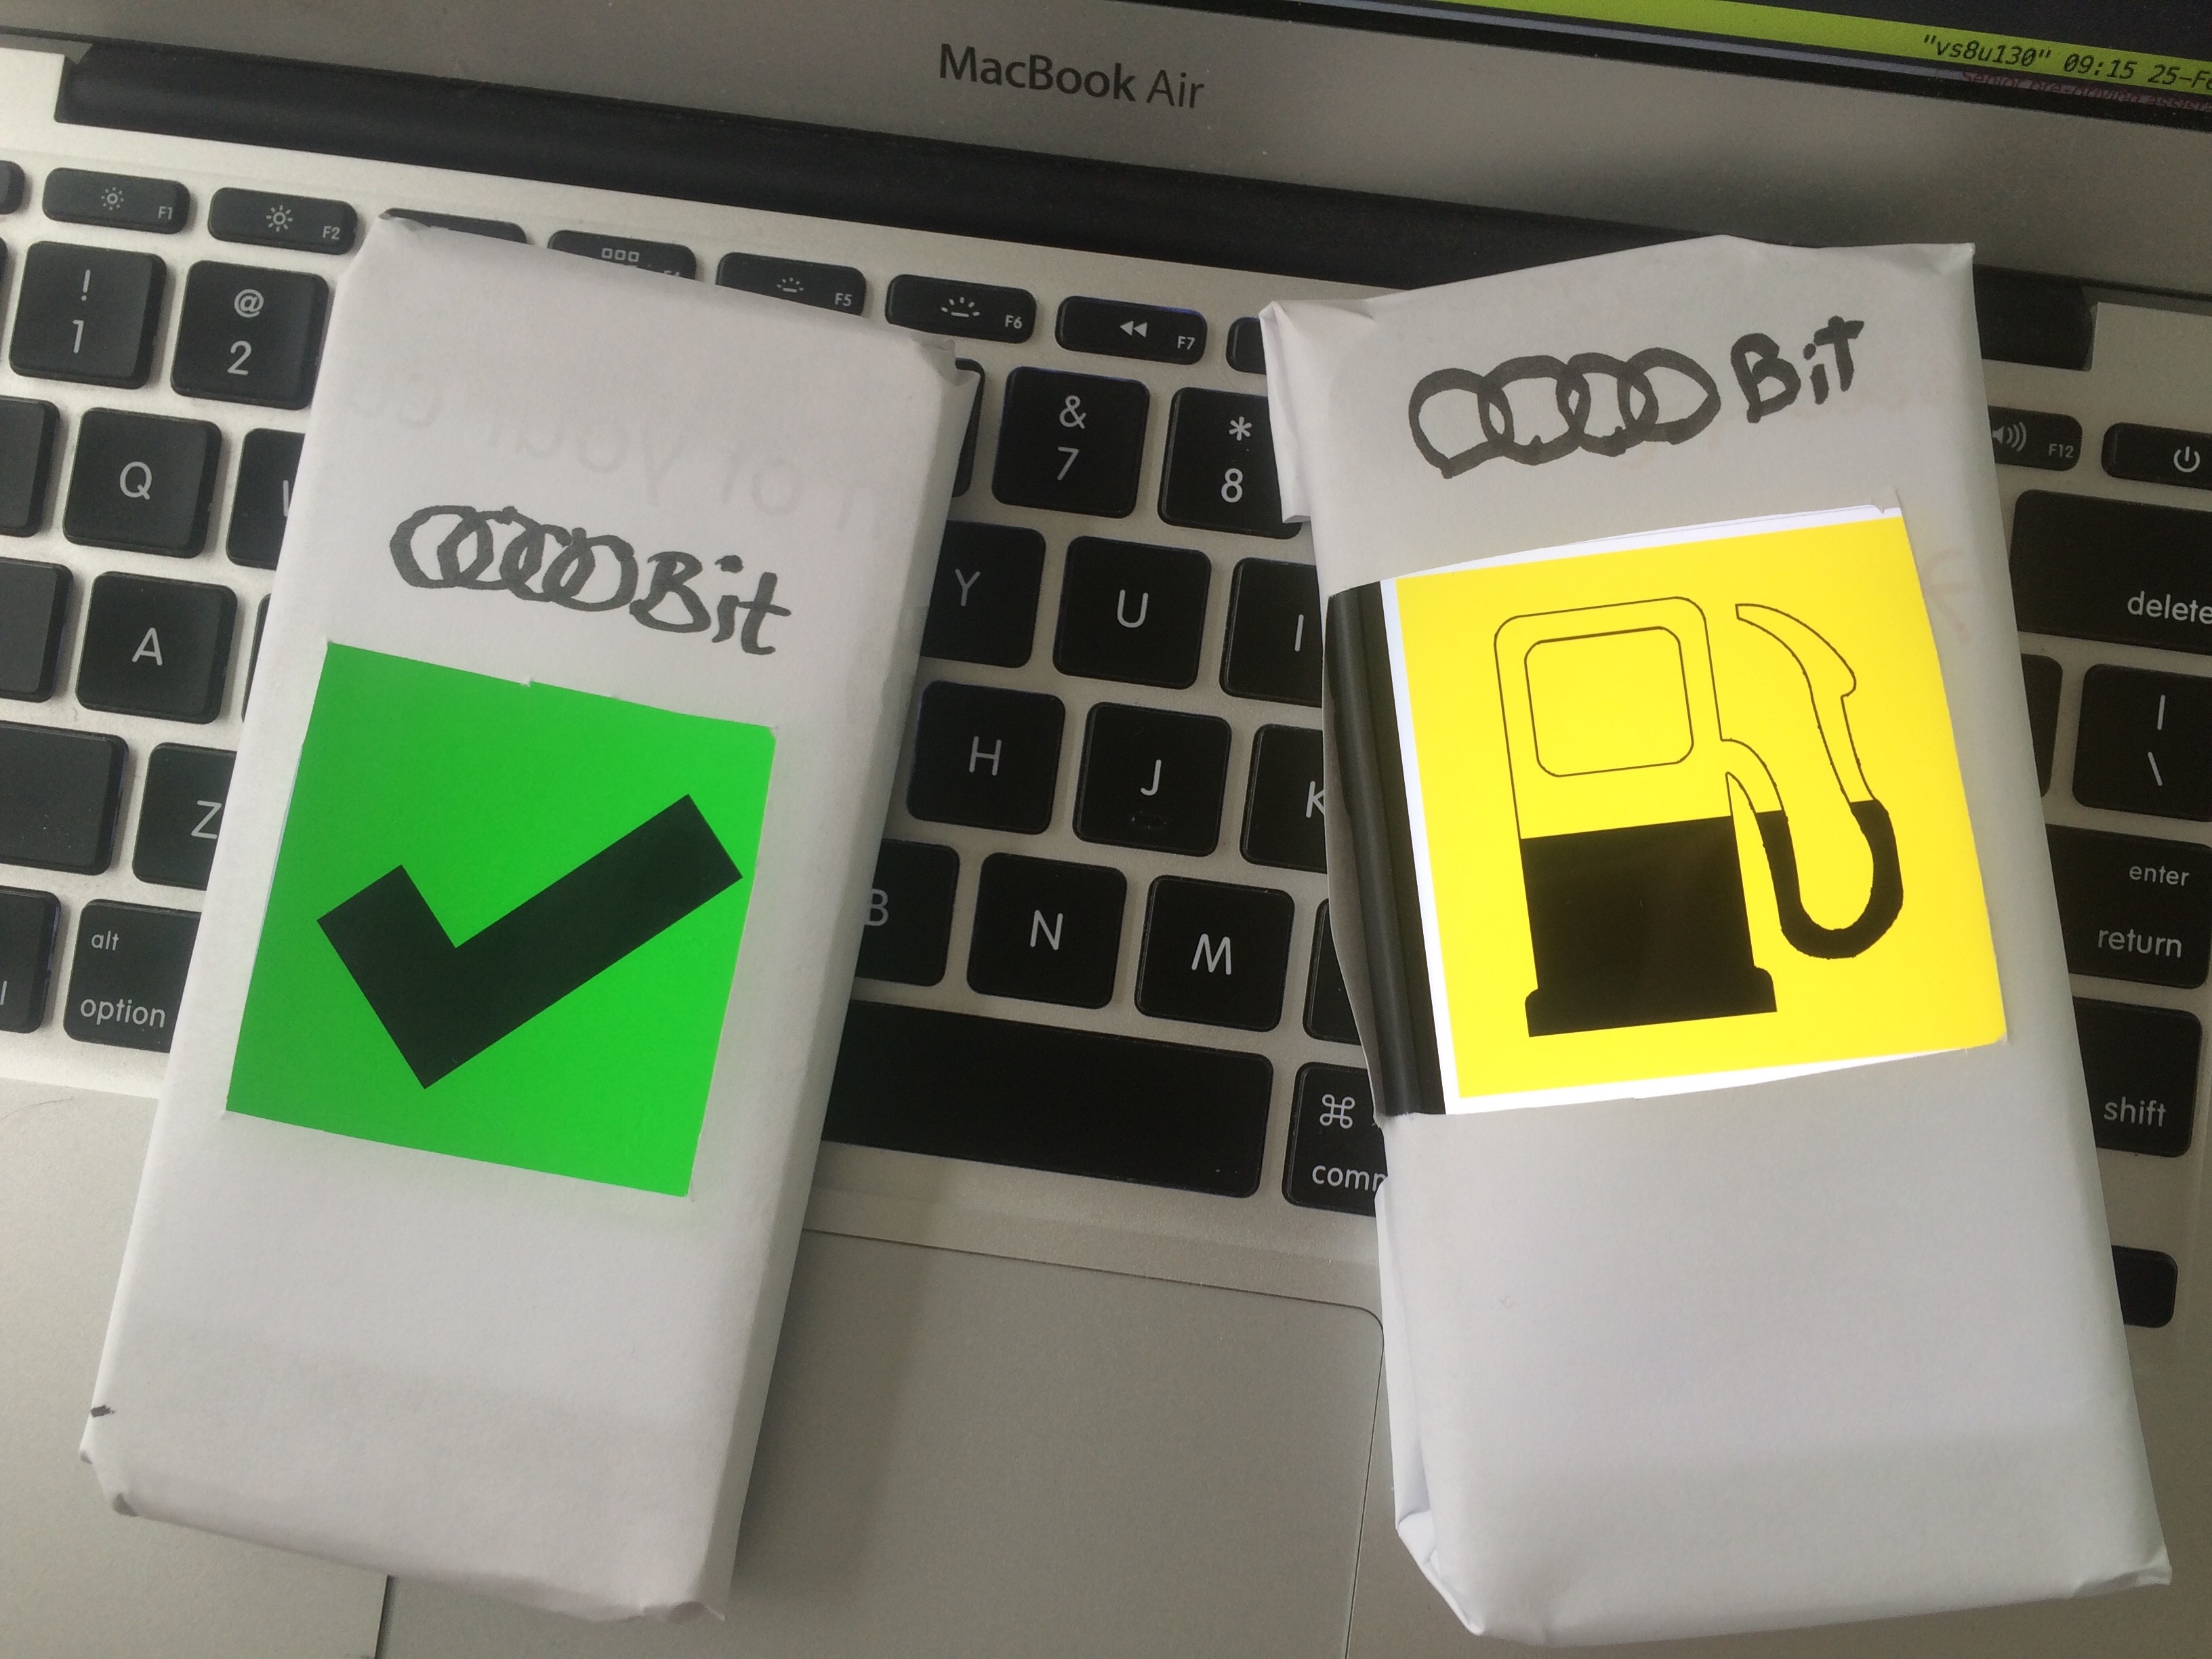
\includegraphics[width=1.0\textwidth]{Figures/AudiBits.JPG}
  \caption{Two \textbf{AudiBits}, the left one displaying an item that the user has packed, the right one displaying the amount of gas left in a user's car.}
  \label{fig:audi_bits_summary}
\end{figure}

\paragraph*{1. Departure} Our main functionality upon departure makes people less forgetful by collecting and making available information to its users about smart home and smart car utilities, as well as personal items, in a meaningful way. This functionality is the result of user interviews and testings, during which we heard that many of those users are forgetful about things like packing, putting their home in a state that enables them to leave, or about things related to their car, like its gas status or where it is parked. AudiSeamless enables display devices like smart phones to ``subscribe'' to utilities and personal items so they get fed with the current status of those. One possible application of this lies in our idea named \textbf{AudiBits}, small displays that show the status of singular items, for example the amount of gas left in a car or whether a user has packed his umbrella (see figure \ref{fig:audi_bits_summary}). Users can specify what AudiBits display, AudiBits in turn suggest useful actions that help users in their daily routine. If an AudiBit detects icy weather and that a user's car is parked outside, it suggests pre-heating the windows so the car owner won't lose time defrosting them. This semi-automation that gives clever suggestions but leaves the user in control is a major aspect of the system and, going forward, we want to further explore its usefulness and applications with users.

\paragraph*{2. Arrival} Upon arrival, AudiSeamless disarms a user's home security system easily by using the presence of a user's car key fob. When a user returns home, all she has to do is place her key fob in a bowl or near a sensor to deactivate the alarm, instead of entering a code, as is standard with current systems.
% {Jonathan} Not relevant for the high-level picture. Here, we only want to show our idea. If somebody is interested in details, they have to read the fine print aka the rest of the document
% Some systems do have wireless key fobs, but the long range signals could easily be intercepted by home invaders and used to deactivate the system.
Owners of home alarm systems produce a lot of false alarms since disarming the system has to be done quickly and can easily result in errors. As a result, many home security systems go unused due to the danger of false alarms, which cost money in public services as well as fines for the homeowner. Our aim with AudiSeamless is to reduce false alarms so that home owners will have reduced costs and lose the urge to disable their alarm system.

% {Jonathan} I think this is too detailed for the executive summary
Users expressed significant interest in having a reason to keep their keys in the same place every day, so that they know exactly where they are. At the moment, there is nothing that ties users' keys to a specific location, so they are often misplaced. Our system should be able to work for both the case if users take their keys out of their pockets when walking in their front door, as well as if they choose to keep them in a bag or purse, as is common with Audi smart key systems, which do not require being placed into a specific place within the car. Only the presence inside of the car is required. Similarly, such a presence inside the home could signal to the home security system that the owner is home. As key fobs are relatively secure and dedicated electronics that verify a user's identity, they offer a convenient and secure way to incorporate smart home functionality into the home through the owner's car, but without compromising integrity of their home lives.

One potential benefit of AudiSeamless is to signal the intent of the Audi owner to their car that they are about to leave. This allows the car to heat up (including electric batteries, which function much more efficiently when heated), connect to the internet to download preloaded directions, and prepare the car's climate if in hot or cold weather. As the user picks up their key fob, the system can send the intention of leaving to the car, and at the same time, a display can remind the user to bring certain belongings if they are not already packed.

These approaches demonstrate a departure from forcing integration with the smart home technology explored last quarter which, while interesting, did not address compelling latent user needs in the team's opinion. Our exploration of the design space this quarter stretches significantly more broadly than last quarter to search for more compelling user needs. However, we believe that we can enhance the experience of arriving and leaving home, specifically addressing the desires of Audi users to have systems that are simple, elegant, not pretentious or showy, and secure.

\begin{figure}[ht]
\label{Fig.AudiDefender}
\centering
	\includegraphics[keepaspectratio, width=5in]{Figures/Specifications/AudiDefender.JPG}
	\caption{The AudiSeamless arrival prototype tested the home security system deactivation with a key fob. The embedded touch screen displayed basic information, analogous to the AudiBits prototype, about the user's car and home.}
\end{figure}

%%%%%%%%%%%%%%%%%%%%%%%%
% TOC and LOF are automatically generated -- Note that you sometimes have to "compile" Latex THREE
% times to update the main .aux files, the TOC etc. files, and finally the PDF output with all changes
% propagated to the printout.
\chaptermark{Contents}
\fakechaptermark{CONTENTS}
%\setcounter{tocdepth}{1}
\tableofcontents*  %asterisk to prevent it from getting a number

% Optional Lists of Figures and Tables:
%\newpage
\listoffigures*  %Note that for this you probably want to add the [short-headings] to captions.
\listoftables*  %I decided to omit the LOT in this example.

%Back to normal size for subsequent sections
%%%%%%%%%%%%%%%%%%%%%%%%

% Set up the Glossary. The template is looking for a file called
% "glossaryterms.tex" with glossary terms and definitions.
\newpage
\chapter*{Glossary}
\fakechaptermark{GLOSSARY}
\label{sec-glossary}
\begin{description}
\item [3D audio technology] Simulation that creates the illusion of sound sources placed anywhere in 3 dimensional space, including behind, above or below the listener.
\item [ADT] A home security and home automation company commonly known as ADT, which originates from "American District Telegraph". ADT offers professionally installed and monitored home security and automation services to users in a subscription model.
\item[Action-event control] Process where a user action creates an physical event.
\item [API] Application Programming Interface - enables other software to use this applications functionality.
\item [Ausim] 3D audio hardware company.
\item [Automatic beam steering] Signal processing technique to narrow the microphone coverage area. Used to pick out a speaker and suppress background noise coming from directions other than that of the speaker.
\item[Benchmarking] A process of researching and observing to understand the state of the art for a given field or topic.
\item[Bluetooth Smart] A wireless personal area network technology specifically designed for low power consumption and low cost.
\item[Brainstorming] A process by which groups of people generate ideas.
\item [Brainwaves] A common term that refers to post-synaptic potentials measured from many neurons in the brain.
\item [California Duster] A brand of car duster made of many fibers that lift dust from the car’s surface to keep it clean between car washes.
\item [CDR] Center for Design Research at Stanford University.
\item [CEP] Otherwise known as a Critical Experience Prototype, this is a prototype built to test an experience that is critical to addressing the problem statement.
\item [CFP] Otherwise known as a Critical Function Prototype, this is a prototype built to test a (technical) function that is critical to addressing the problem statement.
\item [Client] Computer program that accesses a server.
\item [Client-server paradigm] A computing architecture which separates the client from a server over a computer network. 
\item [Connected device] A device equipped with networking capabilities and connected to a network.
\item [Crowded channel] A communication channel that is clogged with information.
\item [CVE] Acronym for Collaborative Virtual Environment. This is a virtual environment that support more than one user at the same time.
\item [Dark Horse] An idea that is unlike the others preceding it, an outlier.
\item [Fitness tracker wristband] A wristband that carries sensors that measure its wearers vital signals to analyze and reflect upon his activity at day and night.
\item [Home Security System] A network of sensors, cameras, and motion detectors that are wired together to determine if unauthorized intruders are entering a home. The system must be armed and disarmed manually by homeowner using a key pad, or in more advanced systems, a smart phone.
\item [HUD] Head-up display --- information is shown on a drivers windshield, without blocking the sight on what lies behind it.
\item [Interaction model] A general concept for a mapping between digital data and the mental models of a user.
\item [Key Fob Case] A cell phone case that contains the electronics of a key fob along with additional connectivity to connect to the phone and home.
\item [Light Therapy] A special kind of light that is designed to mimic the sun's light spectrum, helping to treat users of SAD (see below).
\item[LGM] Large Group Meeting. The weekly meeting of the local ME310- and SUGAR-teams together with the respective teaching assistants.
\item [Low power mesh networks] A network of computers that are connected without a central hub and that consume very little power while doing this.
\item [Meditation Room] A space that is specifically designed to be peaceful and quiet, allowing people to quietly contemplate and find inner peace.
\item [Near Field Communication (NFC)] Radio communication over very short distances that has become the standard platform for contactless payment platforms such as Apple Pay and Google Wallet.
\item[OBD (adapter)] On-Board Diagnostics. An interface that allows to pull certain statistics and data from a vehicle via an adapter such as speed, error codes and pedal position.
\item[Persona] A fictional person representing identified user needs in order to have a reference user for designing the new product. 
\item [Seasonal Affective Disorder (SAD)] A specific type of major depression brought on by changing of the seasons to include more rain and less sun. SAD is often treated with light therapy, traditional therapy, and medication.
\item[Smart home hub] A wireless router type device made by companies like Wink and SmartThings that connects all smart home devices together. This acts as an access point for the mobile phone to control devices.
\item [Smart Key Fob] An electronic key for the car that unlocks the car via proximity sensors. It does not need to be removed from one's pocket or purse to open the car.
\item [Tokenization] The standard security feature of contactless payment systems that ensures security of data using.
\item [Towel Arm] A bundle of microfiber towel held by plastic tongs.
\item [Waterless Car Wash] A solution marketed as an environmentally car wash replacement using very little liquid. Solution is sprayed on car surface and wiped off with a towel - no other rinsing or drying required.   % input the list "glossaryterms.tex"
\end{description}

%%%%%%%%%%%%%%%%%%%%%%%%%%%%%%%%
%% On to the main sections....  Just comment out the \input{} line
%% for any chapters that aren't ready yet.

%%%%%%%%%%%%%%%%%%%%%%%%%%%%%%%%
%MRC5December2012 -- Added a bit about  the corporate partner context
%Context
\chapterimage{ChapterImages/context}
\chapter{Context}\label{sec-context} %Label for cross-referencing

% %%%%%%%%%%%%
% \begin{remark} \color{blue}
% {\Large What need are you addressing for your users and your company?}

% \noindent The Context provides background and motivation for your project. It is an enlarged version of the brief context in your Executive Summary.  
% \begin{itemize} %\tightlist
% \item Who came to you with a proposed project area? Who is the corporate partner and what is their context?
% \item What background or context set the stage for your Needfinding and Benchmarking, activities?
% \end{itemize}
% Suggested length: Up to half a page to a page each for the Need Statement and Problem Statement (plus figures, if any). Another page or two for the design team.
% \normalcolor \end{remark}
% %%%%%%%%%%%%

\section{Design Challenge}
\label{sec:challenge}

The technology around home and car has changed dramatically in the last decade with autonomous driving, voice control and the Internet of Things (IoT) being the most prominent of these developments. For this project, we were given the following challenge: With the smart home promising a future of convenience and intelligence at home, what could the future hold for Audi?

\todo{picture for business canvas looks cutoff at top and has icons in lower left}

\begin{figure}[ht]
	\centering
	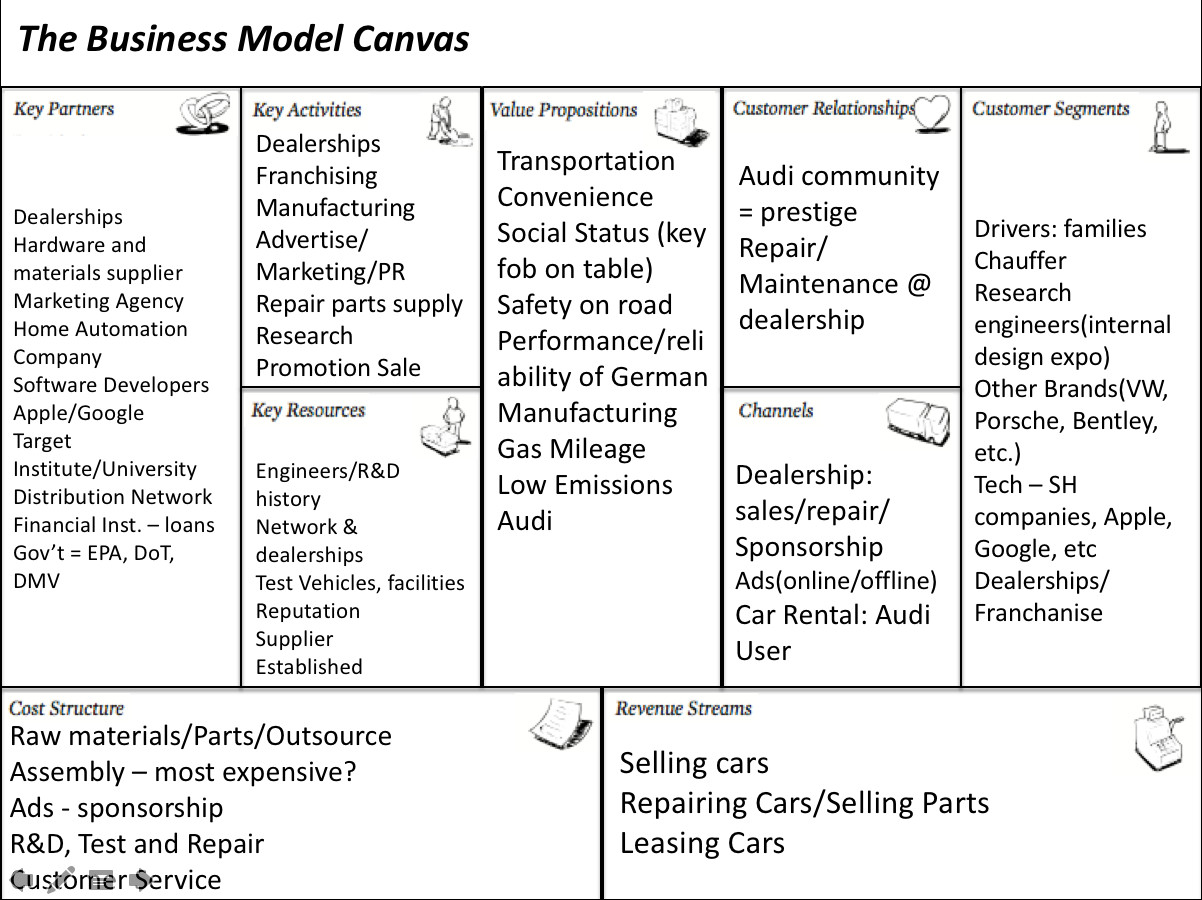
\includegraphics[width=5.9in]{Figures/ChapterContext/canvas.png}
	\caption{The business canvas that identifies the business model of Audi and related stakeholders}
	\label{fig:canvas}
\end{figure}

\section{Problem Statement}

The focus of our work is to create an integration of the Audi brand into the smart home. Most desirable would be a physical representation of Audi in the home since that would expand Audi's perceived value beyond that of a car maker. This brings up the question that we currently work on:

\begin{center}
\textbf{How can Audi play a meaningful role in the emerging smart home market\\or integrate itself with the promises of smart home technology?}
\end{center}

\section{Corporate Partner: Audi}
\label{subsec:audi}

The automobile manufacturer Audi is the corporate partner for this project. As a major producer of luxury cars, Audi has always been at the forefront of automobile technology -  both in driving experience and comfort features of the car. The latest technological innovations are usually implemented into the most expensive series first. Subsequently, they make their way down the line-up, appearing in more affordable models every year. Audi produces a wide range of vehicles from sedans to sport utility vehicles ~\cite{Audi2014Winter}.

Fig. \ref{fig:canvas} describes the team's understanding of the Audi brand and the Volkswagen corporation. As a traditional car manufacturer, Audi's revenue mainly comes from selling cars, its cost consists of raw materials, machining, assembly, advertisement, Research and Design (R\&D), test and customer service. Audi's key resources are threefold: first is the work of engineers and its R\&D achievements, second is its distribution network and dealerships, and third is its brand and reputation. The key value proposition of Audi is convenience and fun of driving, being considered a social status symbol, delivering great performance, as well as providing the reliability of German engineering and its experience with advanced technology.
% \begin{remark} \color{blue}
% \textit{I didn't understand this sentence and hope I could capture its meaning with the following paragraph (I would argue that prestige is already captured in "social status symbol" of the preceding paragraph):}
% Audi has a emphasis on custom relationship, because Audi community has a closely emotional bond to this brand, and an important part of the luxury brand is the prestige.
% \end{remark}
Audi maintains good relationships with customers who develop an emotional bond to it, making the relationship mutually beneficial.

%If possible, try to make this display on a whole page


The Electronics Research Laboratory (ERL) is the main contact point between the design team and Audi. It is is the direct link of Audi and other Volkswagen Group brands to Silicon Valley. Engineers here are encouraged to invent and experiment with innovative technological solutions and features that explore the opportunity space for future car generations. At the same time, the location benefits vastly of the proximity to the main drivers of the IT industry and elite educational institutions. Relevant research areas include human machine interface systems, driver assist systems, and infotainment applications and platforms ~\cite{Audi2012December}.

\begin{center}
% * <djmoore3@stanford.edu> 2015-12-10T16:37:20.003Z:
%
% > \begin{center}
% > 
\includegraphics{Figures/AUDI}
% > \vfill
% > 
\includegraphics{Figures/ERL}
% > \end{center}
%
% Can these graphics be better laid out?
%
% ^.


\includegraphics{Figures/Logos/AUDI}

% \vspace{1cm}


\includegraphics{Figures/Logos/ERL}

\end{center}

\clearpage

\subsection{Corporate Liaisons}

\vspace{1em}
\noindent 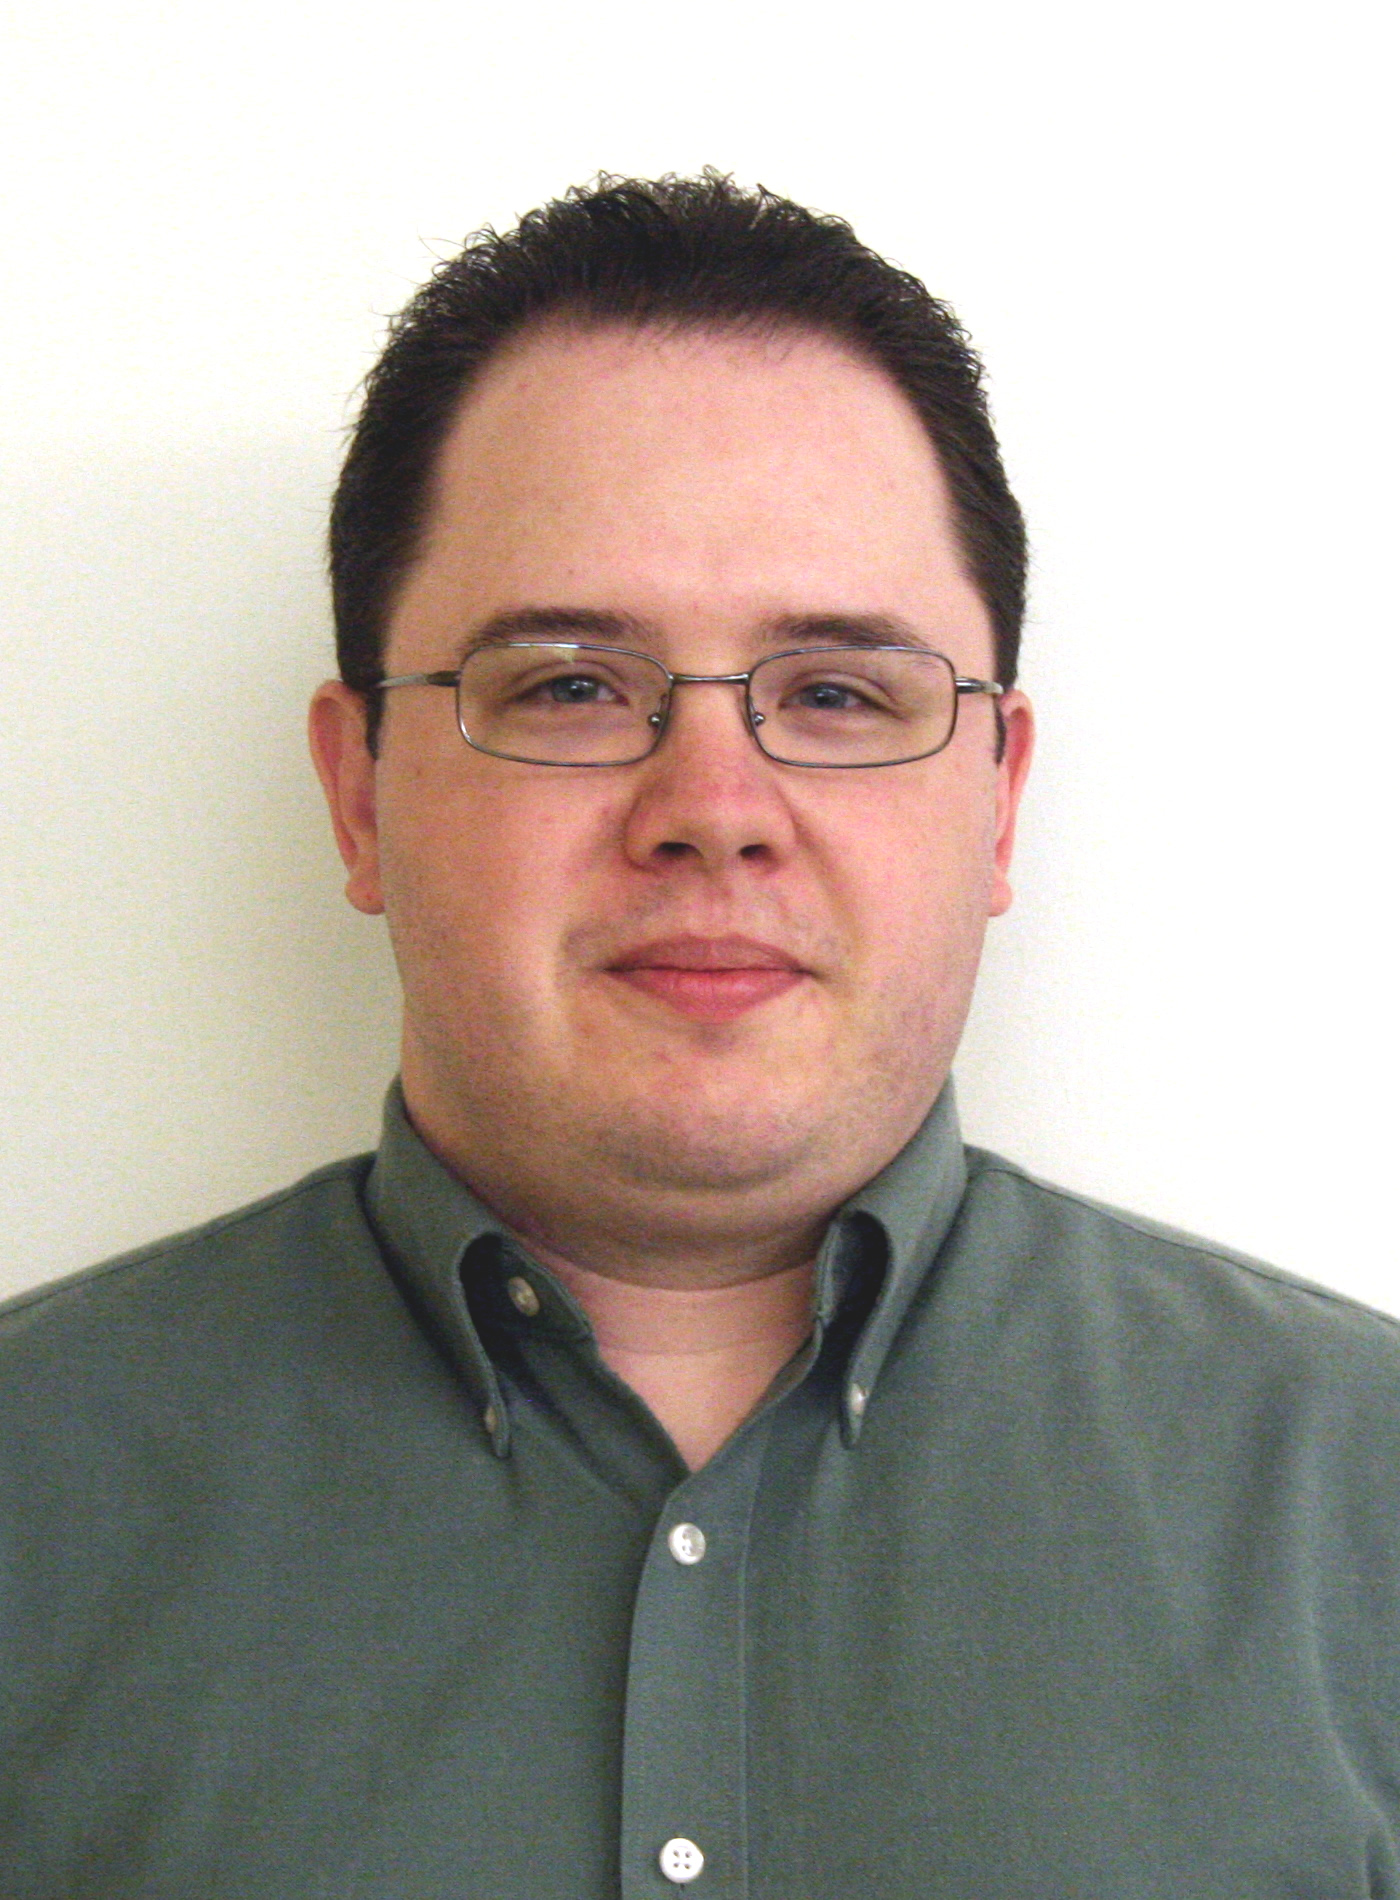
\includegraphics[width=35mm]{Figures/People/Nate}
\hspace{1em}\parbox[b]{0.6\textwidth}{\textbf{Nathaniel Coser}\\
Volkswagen-Electronics Research Laboratory\\
Contact: Nathaniel.Coser@vw.com\\
}
\vspace{2em}

\noindent 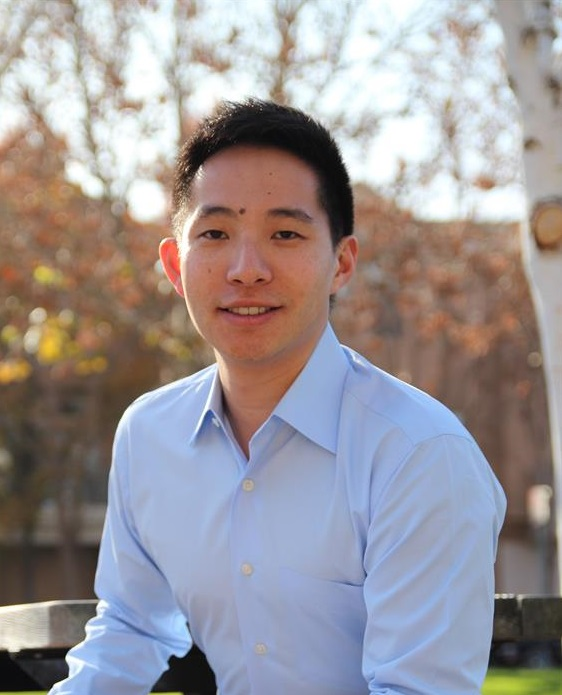
\includegraphics[width=35mm]{Figures/People/andrew}
\hspace{1em}\parbox[b]{0.6\textwidth}{\textbf{Andrew Chang}\\
Volkswagen-Electronics Research Laboratory\\
Contact: Andrew.Chang@vw.com\\
}
\vspace{2em}

\noindent 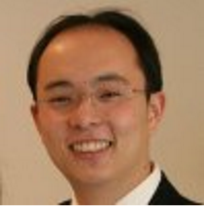
\includegraphics[width=35mm]{Figures/People/Henry}
\hspace{1em}\parbox[b]{0.6\textwidth}{\textbf{Henry Chen}\\
Volkswagen-Electronics Research Laboratory \\
Contact: Henry.Chen@vw.com\\
}

\clearpage

\section{The Design Team}
\label{sec:team}

The design team was assembled from individuals with a diversity of thinking preferences, interests and backgrounds. There is some evidence that such diversity enhances team creativity \cite{Wilde97, Wilde07} , even if it creates additional challenges for team management.

\subsection{Students}

% Example table. It gets a caption and reference label.
% The tabular formatting is a bit painful...  An alternative is to use Word
% and insert the PDF printout as for a figure. There are also Word-to-Latex converters.
%
%Nov2013 -- I decided to comment this out because corporate partners don't care about this. -MRC
%
%\begin{table}
%  \begin{tabular}{| p{14mm} | p{20mm} | p{20mm} | p{22mm} | p{20mm} | p{12mm} |} 
%  \hline
%Score & Extroverted-Introverted (E-I) & Intuition-Sensing (N-S) & Feeling-Thinking (F-T) & Perception-Judging (P-J) & Overall \\
%People & & & & &\\
%\hline
%Larry & +6 & +6 & -6 & +12 & ENTP \\
%Mark & -18 & +30 & -30 & +18 & INTP \\
%George & +6 & +18 & -18 & +6 & ENTP \\
%\hline
%\end{tabular}
%\caption{Team preferences scores using the method of Wilde \cite{Wilde07}. (These data are not real.)}
%	\label{wildeprefs}  %Tag for referring to table
%\end{table}

%\begin{framed}
%\noindent \includegraphics[width=40mm]{Figures/Ch2/LarryLeifer.jpg}
% \parbox[b]{0.6\textwidth}{Larry Leifer\\
% Status: Professor, Mechanical Engineering\\
% Contact: leifer@cdr.stanford.edu\\
% Skills: deisgn, mechatronics, welding, prototyping\\
% Computing: Solid Works, Matlab, basic C programming, Forth\\
% }
% %Note, the blank lines matter - they cause the start of a paragraph in the box.

% Born in Santa Barbara I remain a surfer at heart.
% My research is focused on instrumenting, understanding, supporting, and improving design practice through the development of design theory. BS in in Engineering Science, MS in Product Design, PhD in Biomedical Engineering, all from Stanford.
% Founder of the  Center for Design Research and one of the founding faculty members of the Hasso Plattner Design Institute
% at Stanford (aka the d.school).

% Favorite activities include surfing, hunting and wayfaring, and frequent trips to Lucerne, Switzerland.
%\end{framed}

%\begin{framed}
\vspace{0.5em}
\noindent 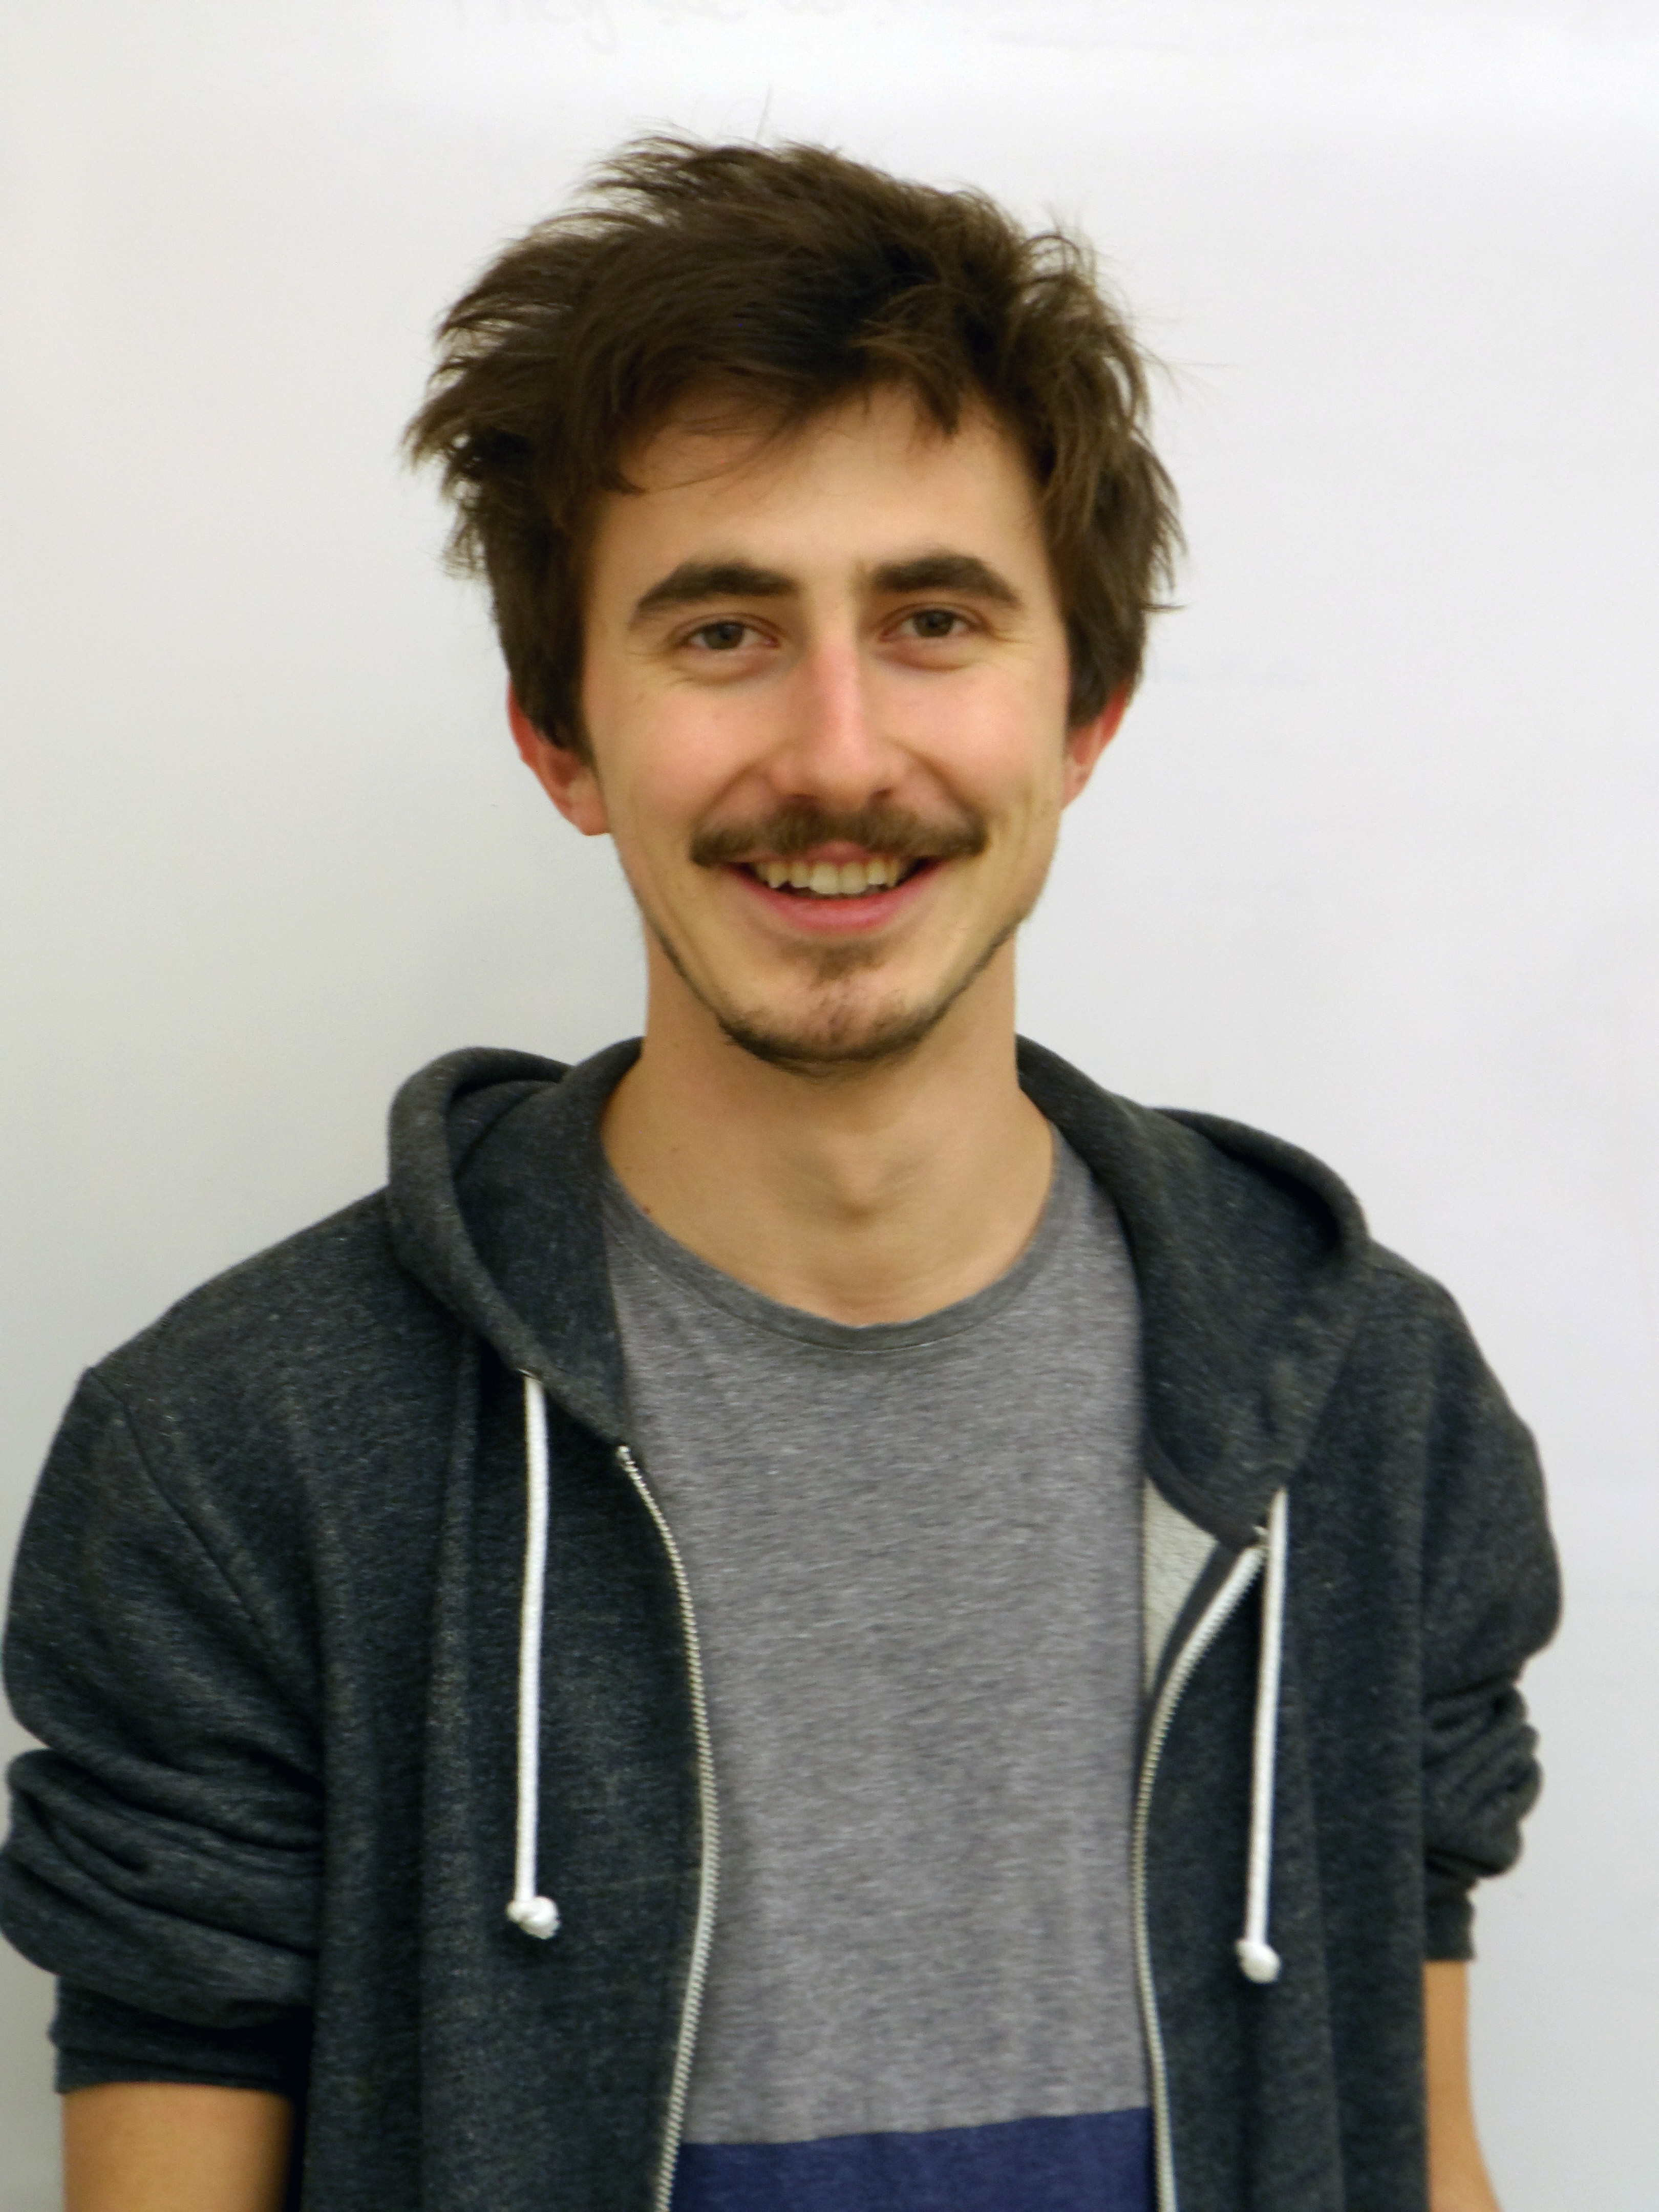
\includegraphics[width=35mm]{Figures/People/martin}
\hspace{0.5em}\parbox[b]{0.6\textwidth}{\textbf{Martin Fritzsche}\\
Hasso Plattner Institute\\
Status: IT-Systems Engineering Master's degree student\\
Contact: martin.fritzsche@student.hpi.de\\
Skills: Software Engineering, Human Computer Interaction, C++\\
}

I was born 1989 in the medium sized town Jena in the center of Germany. After finishing school there and spending a year in Dresden working in a hospital for civil service I started my studies at the Hasso Plattner Institute (HPI). In 2012, in between Bachelor and Master at HPI, I collected valuable working experience as full-time employee at Citrix Online Germany. In my masters studies I focused on human computer interaction, working on prototyping research and combining virtual reality with real life by taking control of the users muscles. Before starting the ME310 course this fall I spent one year at Universidad Politécnica de Madrid in Spain.

Besides virtual reality research and low level development I like hands-on experiences and interdisciplinary work. That is why I am happy to dive into the design thinking process and work on our real life project at ME310.
%\end{framed}

\vspace{2em}
\noindent 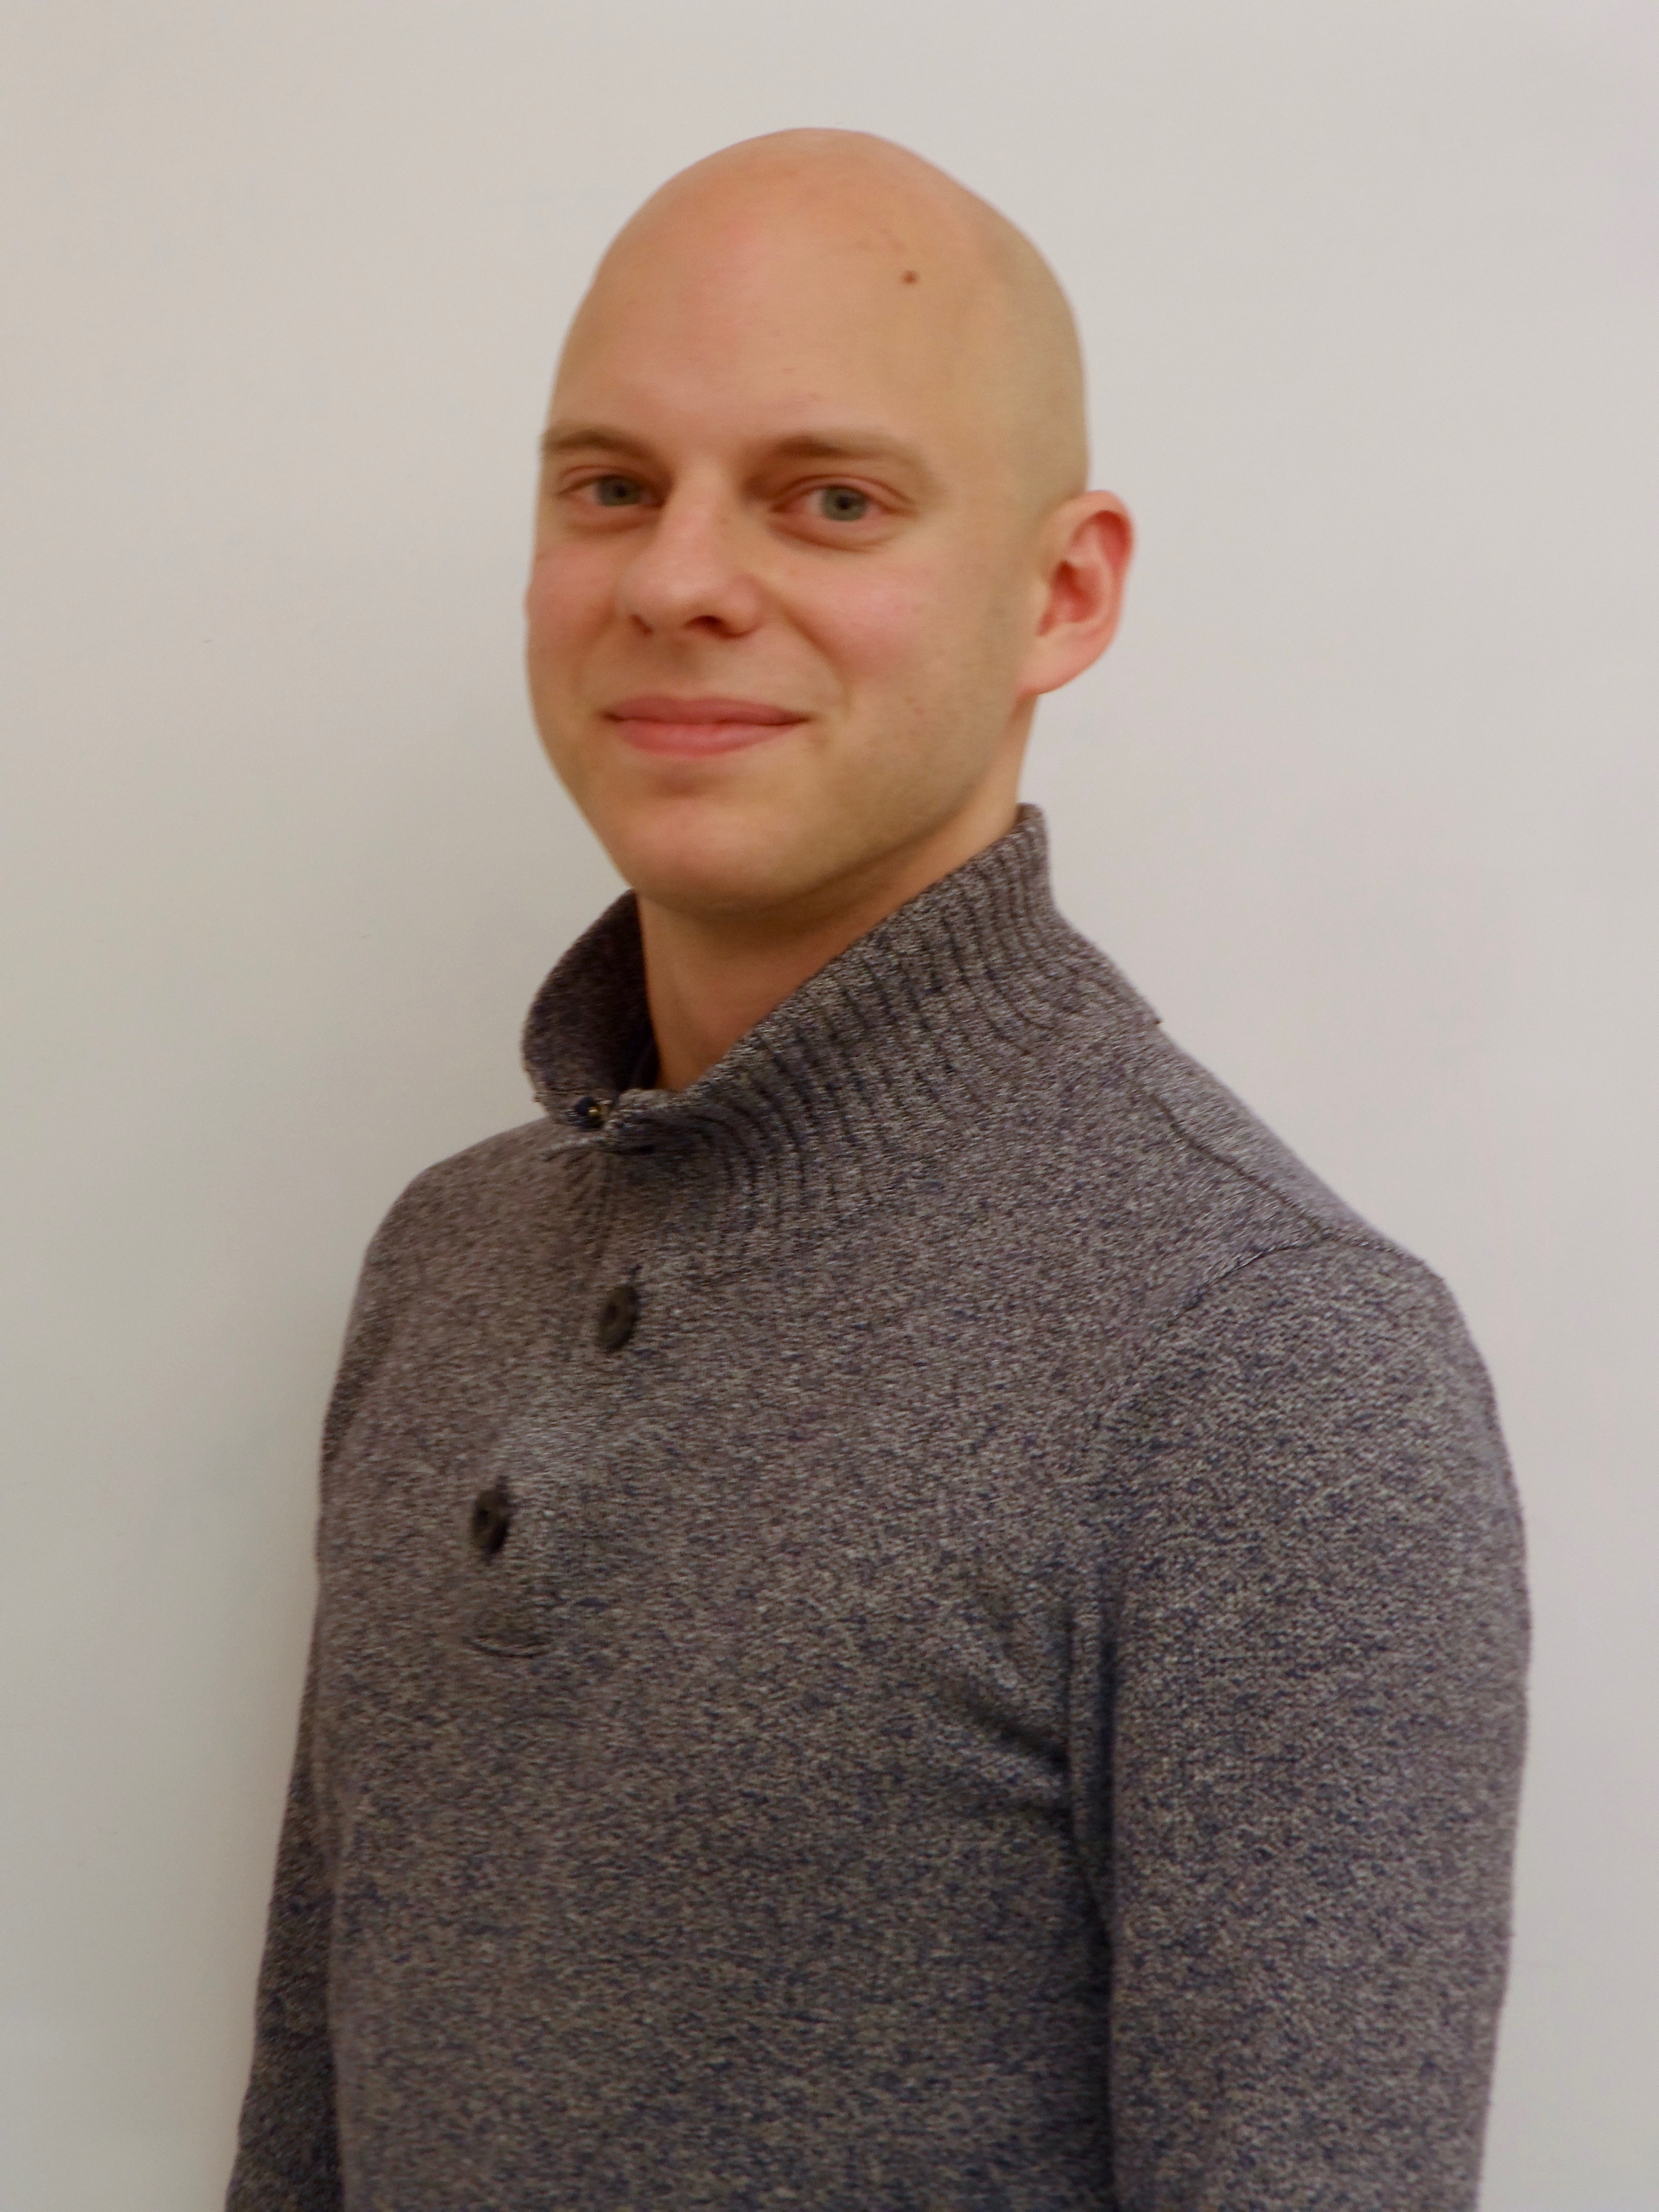
\includegraphics[width=35mm]{Figures/People/Jonathan}
\hspace{0.5em}\parbox[b]{0.6\textwidth}{\textbf{Jonathan Herdt}\\
Hasso Plattner Institute\\
Status: IT-Systems Engineering Master's degree student\\
Contact: jonathan.herdt@student.hpi.de\\
Skills: Design Thinking, Computer Science\\
}

I come from the Rhine-Neckar Metropolitan Region in Southern Germany and was born in Mannheim. Professionally, Heidelberg University was my first step to becoming a computer scientist because I completed a three year training there to become a computer science expert. I then earned my B.S. in Computer Science at Hochschule Mannheim (now also part of the SUGAR network). During my time as a student at Hochschule Mannheim, I spent two semesters abroad --- one in the US (College Park, MD) for an internship at Fraunhofer and one in Canada (St. John's, NL) for studying. I aim to take my education to another level by pursuing my M.S. in IT-Systems Engineering at Hasso Plattner Institute.

My main interest in my professional life is to create simple solutions. I enjoy getting to the heart of people's interactions with technology and what makes these interactions work or not work. This path has led me to discover Design Thinking for myself which goes a long way to ensuring that a user is at the heart of every creation and enhances my focus on simplicity with satisfying unfulfilled desires. ME310  was the next logical step in this direction for me and the outcome so far has shown me that this was the right decision.

%\begin{framed}
\vspace{2em}
\noindent 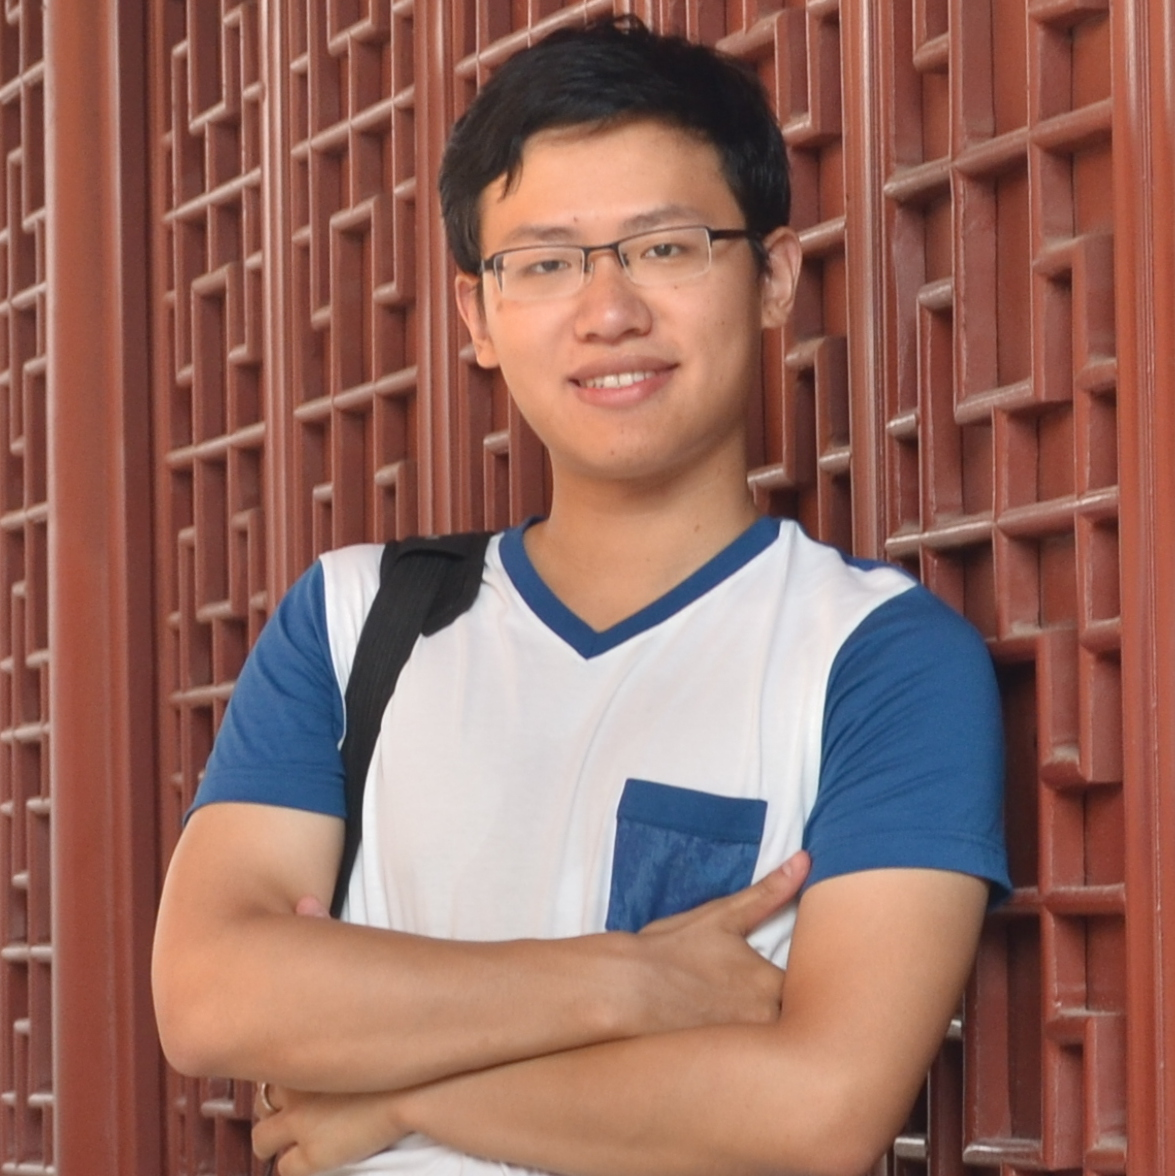
\includegraphics[width=35mm]{Figures/People/Zhipeng}
\hspace{0.5em}\parbox[b]{0.6\textwidth}{\textbf{Zhipeng Hu}\\
Stanford University\\
Status: M.E. first year Graduate Student\\
Contact: zhipengh@stanford.edu\\
Skills: Design, Mechatronics, Programming\\
}

I was born in Wuhan, a metropolis in the middle of China. I earned my Bachelor of Engineering degree in Mechanical Engineering at Tsinghua University, China.

I am interested in Mechatronics and Design. More specifically, I am fascinated by creative solution at systematic level and the interdisciplinary nature of Mechatronics area. As a Bachelor student, I have engaged in various design projects with topics such as embedded system, mechanical design, and virtual instrument. These experiences inspired me to further explore possibilities of smart product design, especially those within practical background. Moreover, during my undergraduate studies, I have focused on control theory and algorithms with application on precision motion control. It convinced me that smart products need a combination of hardware design and control software, which can be successfully integrated using design thinking.

%\end{framed}

%\begin{framed}
\vspace{2em}
\noindent 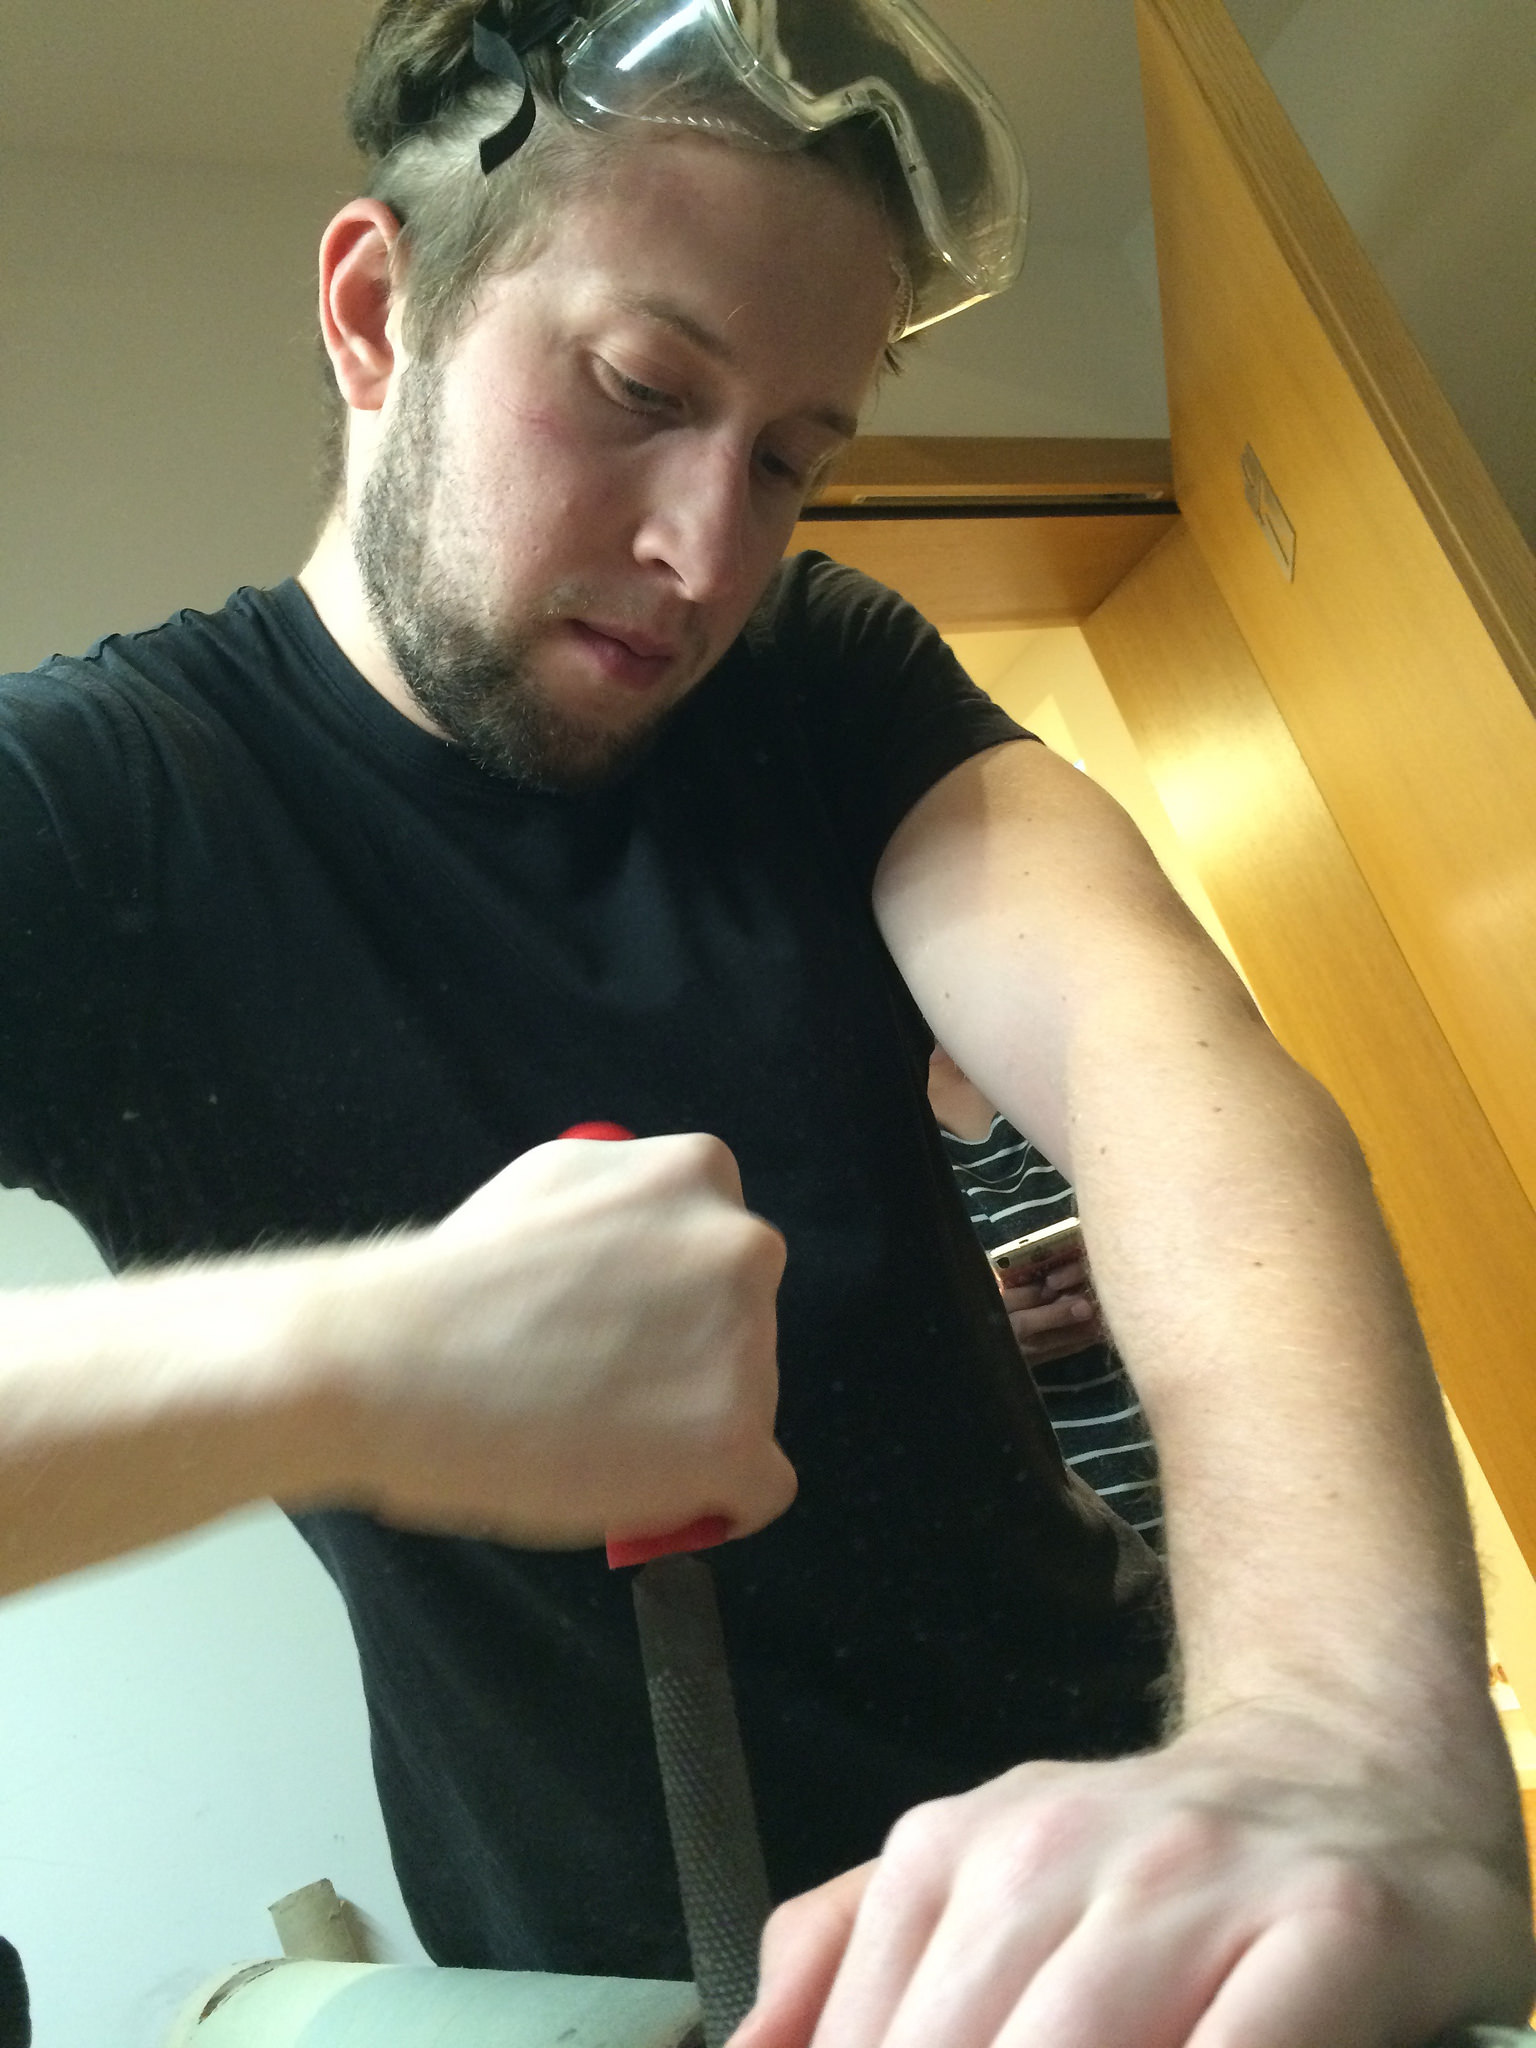
\includegraphics[width=35mm]{Figures/People/Jonas}
\hspace{0.5em}\parbox[b]{0.6\textwidth}{\textbf{Jonas Kemper}\\
Hasso Plattner Institute\\
Status: IT-Systems Engineering Master's degree student\\
Contact: jonas.kemper@student.hpi.de\\
Skills: Programming, Prototyping, Interaction design\\}

Born and raised in Germany near Cologne, I earned my Bachelor of Science degree from LMU Munich in Media Informatics and Human-Computer Interaction. Before starting to pursue a Master's degree at HPI, I programmed for and wrote my Bachelor's thesis about a cognitive architecture now based at MIT media lab. To continue this work, I was invited to attend two workshops held at the media lab (five weeks in 2014 and two weeks in 2015). I spent two quarters as a visiting computer science graduate student at UC San Diego where I also worked part-time at the design lab.

My interests span communication technology, concept development, and the business side of technology. These plus the multidisciplinary teams and the international community are why I am excited about the ME310 opportunity.
%\end{framed}

%\begin{framed}
\vspace{2em}
\noindent 
\includegraphics[width=35mm]{Figures/People/Johanna}
\hspace{0.5em}\parbox[b]{0.6\textwidth}{\textbf{Johanna Latt}\\
Hasso Plattner Institute\\
Status: IT-Systems Engineering Master's degree student\\
Contact: johanna.latt@student.hpi.de\\
Skills: Software Engineering, Mobile and VR Applications, Human Computer Interaction\\
}

I was born in Siegen, a city near Cologne, and grew up in a little village of 2,500 residents. I received my Bachelor of Science degree in Human-Computer Interaction from the University of Würzburg in Bavaria. Next to basics as psychology and methods of human-computer interaction, I also learned the basics of software engineering and worked in an IT company focusing on semantic web technologies during my time as undergraduate. In my bachelor thesis I worked on the topic of illusion of body ownership in virtual realities. Since I really enjoyed the computer science part of my studies I decided to apply at Hasso Plattner Institute for my master's degree, where I am currently in my 2nd semester.

I am fascinated by the human-centered design-thinking process of finding user needs and problems to develop meaningful and innovative applications and I love having the opportunity to walk through the full design cycle in the ME310 course, from the basic benchmarking and needfinding to the finished product, which unites my interests in psychology and computer science.
%\end{framed}

\vspace{2em}
\noindent 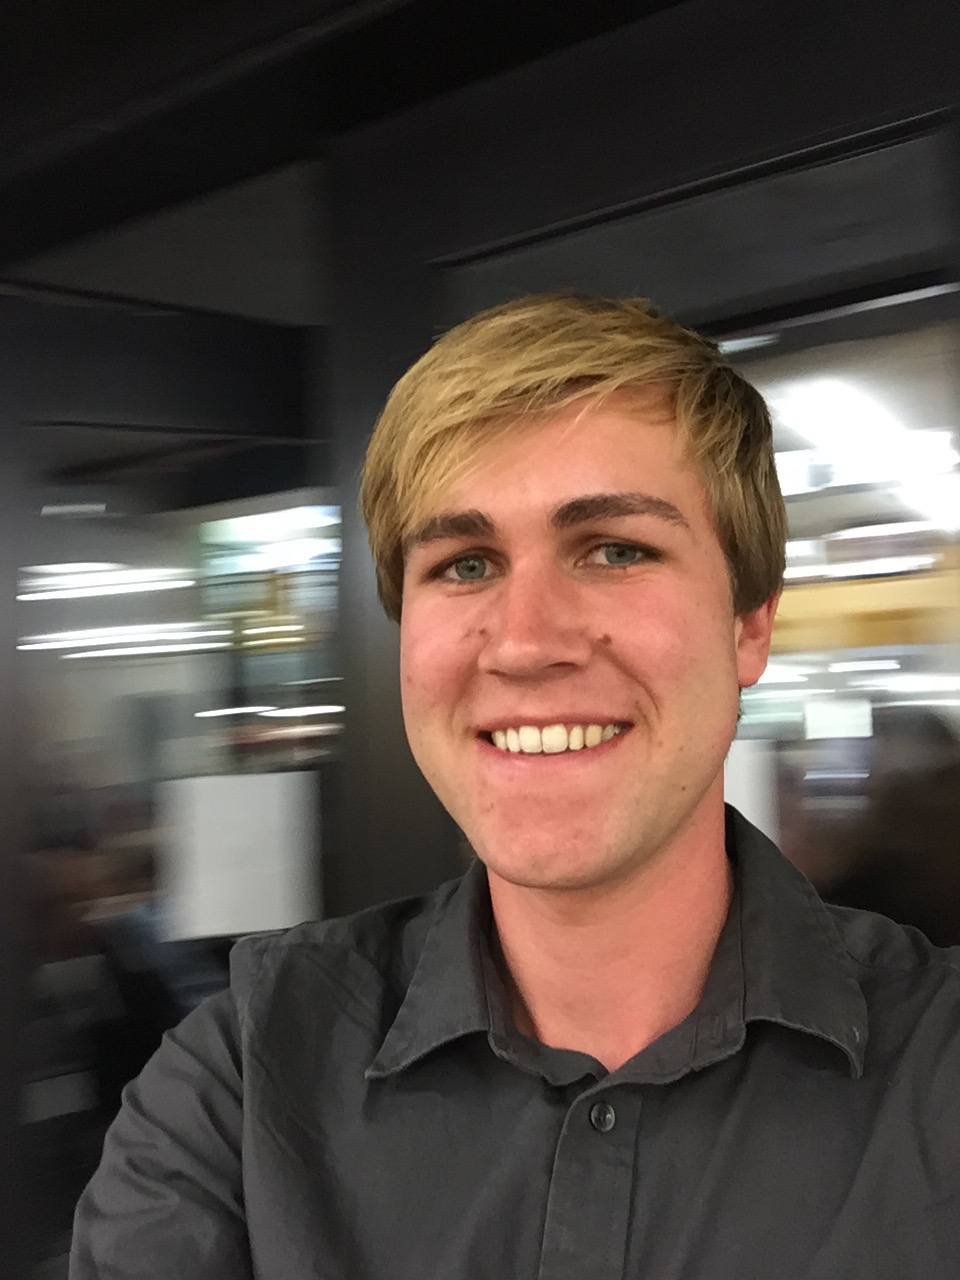
\includegraphics[width=35mm]{Figures/People/Dylan}
\hspace{0.5em}\parbox[b]{0.6\textwidth}{\textbf{Dylan Moore}\\
Stanford University\\
Status: First Year Mechanical Engineering Ph.D. Student\\
Contact: djmoore3@stanford.edu\\
Skills: Conceptual Design, User Experience, Systems Engineering, Research, Design Methodology, Graphic Design\\
}

I was born in Laguna Beach, CA and grew up in Orange County, CA. I received a B.S. in Engineering Physics and a B.A. in Music from UC Berkeley while an undergraduate and spent a summer studying abroad at the University of Cambridge in England. After Berkeley, I completed a Master’s at USC in Mechanical Engineering. I currently perform research on the design process in Professor Erin MacDonald's IRIS Design Lab. In the past, I have held several engineering internships and participated in research projects in the IMPACT laboratory at USC and Lawrence Berkeley National Lab.

I am incredibly curious about the world we live in, and I am interested in contributing to society in as many ways as I can.  I have a passionate drive for divergent creativity and problem solving, and I am excited about the opportunities and  experience ME310 offers. I bring a holistic and systems-level approach to the design team and look to integrate everyone's unique experience and perspectives into a unified vision.

%\end{framed}

\vspace{2em}
\noindent 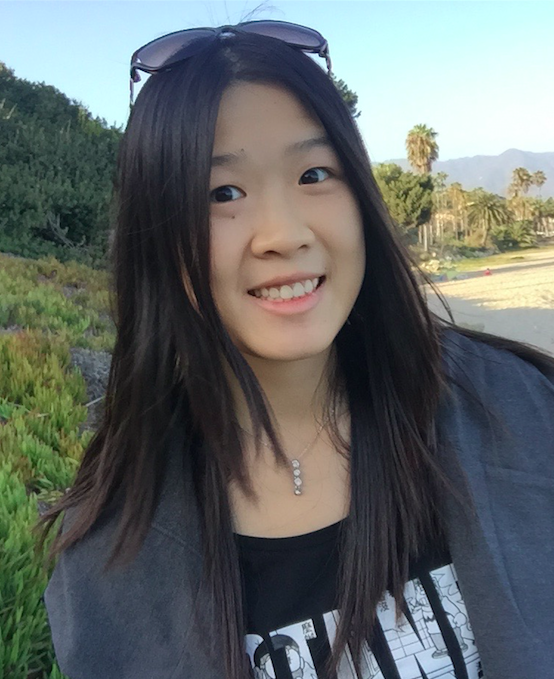
\includegraphics[width=35mm]{Figures/People/Maggie_Xu.png}
\hspace{0.5em}\parbox[b]{0.6\textwidth}{\textbf{Maggie Xu}\\
Stanford University\\
Status: First Year Mechanical Engineering Master Student\\
Contact: manqixu@stanford.edu\\
Skills: sketch, C++, violin\\
}

I grew up in China and received a B.S. degree in Mechanical Engineering from Tsinghua University in 2015. I'm interested in trying out new ideas and building stuff. I'm also curious about how the engineering design process could be improved through the interaction with other fields like physiology, humanity, or social science. My undergraduate major is precision instruments so most of my past design experiences are more focused on tiny devices like microchips for medical use. I had some mechatronics design experiences through class. I was an undergraduate visiting researcher at Stanford Mechanical Engineering Research Lab (MERL) in the summer of 2014, working on a droplet-based microfluidic chip for quantitative bacteria detection. In the winter of 2015, I was a research intern at the Centre for Advanced Photonics and Electronics (CAPE) at Cambridge University, designing the next generation of a star tracking system based on compressive sensing. Besides research, I've also completed a four-month marketing internship at Daimler AG, where I had a lot of fun and enjoyed the opportunity of understanding Mercedes-Benz cars from both an engineering side and a marketing side did help a lot in generating advertising ideas.
%\end{framed}

\clearpage

\subsection{Coaches}

\vspace{0.5em}
\noindent 
\includegraphics[width=35mm]{Figures/People/Scott_Henkelman.jpg}
\hspace{0.5em}\parbox[b]{0.6\textwidth}{\textbf{Scott Henkelman}\\
Scott Henkelman\\Stanford University\\
Status: Product Engineer, Private Technology Company\\
Contact: sjhenk@gmail.com\\
}
% \end{framed}

\vspace{2em}
\noindent 
\includegraphics[width=35mm]{Figures/People/Max}
\hspace{0.5em}\parbox[b]{0.6\textwidth}{\textbf{Max Bothe}\\Hasso Plattner Institute\\
Status: IT-Systems Engineering Master's degree student\\
Contact: max.bothe@student.hpi.de\\
Skills: Software Engineering, iOS Development, Python\\
}

I was born in 1990 in a small town in Brandenburg, Germany. In 2009, I moved to Potsdam to start my Bachelor's studies at the Hasso Plattner Institute. Afterwards I joined SAP in Belfast, Northern Ireland, for software engineering internship for six months.
Currently I am again a computer science student at the Hasso Plattner Institute for getting my Master's degree. As part of my studies I am also working as a student assistant in the field of soccer analytics on databases.

I am interested in software engineering, iOS development, project management and creative design. I joined ME310 in 2014 developing a prototype of the must have features of the Audi ownership experience in 2025.

%\end{framed}

\section{What is ME310?}

\subsection{Design Thinking}

Design Thinking is the latest successor in a long-ranging history of research and development on design methods. More than half a century ago, in the mid-1960s, a need for a structured design process arose due to the rising complexities of developing technologies\footnote{Beckman, Sara L., and Michael Barry. "Innovation as a Learning Process: Embedding Design Thinking." (2007).}. Herbert Simon was the first to describe design as a "way of thinking"\footnote{Simon, Herbert Alexander. The sciences of the artificial. MIT press, 1969.}. Design Thinking grounds in the observation of how designers approach problems and how they develop new solutions\footnote{Cross, Nigel. Designerly ways of knowing. Springer London, 2006.}. 

According to David and Tom Kelley "Design Thinking is a way of finding human needs and creating new solutions using the tools and mindsets of design practitioners"\footnote{Kelley, Tom, and David Kelley. Creative confidence: Unleashing the creative potential within us all. Random House LLC, 2013.}. Design Thinkers combine empathy for the context of a problem, creativity in the generation of insights and solutions, and rationality in analysing and fitting various solutions to the problem context.
Although many tried to define what Design Thinking is\footnote{Razzouk, Rim, and Valerie Shute. "What is design thinking and why is it important?." Review of Educational Research (2012): 0034654312457429.}, there is still uncertainty whether to describe it as a methodology, a process or a mindset. For the sake of clarity we define Design Thinking as a methodology, attributed by three core elements: multidisciplinary teams, an iterative process and variable space (see figure~\ref{fig:d_process}).

\begin{figure}
  \centering
    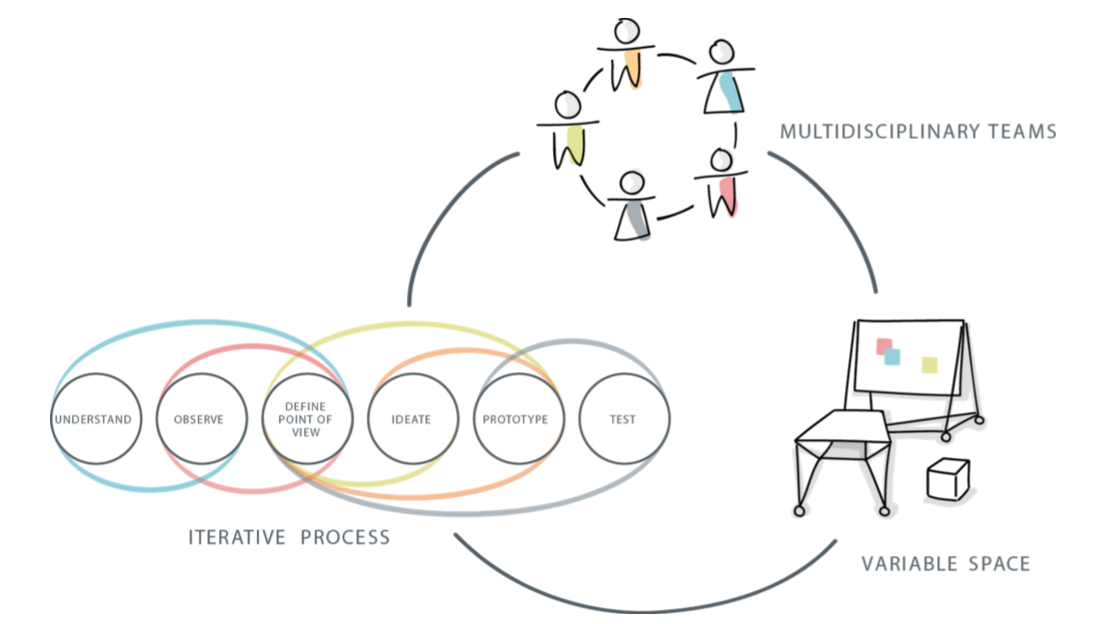
\includegraphics[width=1.0\textwidth]{Figures/ChapterContext/d_process}
  \caption[The Design-Thinking process]{© Prof. Ulrich Weinberg/HPI School of Design Thinking}
  \label{fig:d_process}
\end{figure}

\subsubsection{Process}

Kumar argues that "successful innovation can and should be planned and managed like any other organisational function"\footnote{Kumar, Vijay. 101 design methods: A structured approach for driving innovation in your organization. John Wiley \& Sons, 2012.}. And although his definition of the design process is different from Design Thinking, all approaches to design share great similarity in their attributes, e.g. being human-centered, non-linear, iterative and incremental. Brown explains the "continuum of innovation as a system of overlapping spaces called inspiration, ideation, and implementation"\footnote{Brown, Tim. Change by design. HarperCollins e-books, 2014.}, as opposed to a "predefined series of orderly steps". 

We use this iterative process to find out about people's hidden needs and match those with what is technologically feasible and what is viable in terms of business strategy. Key to the process is the strict separation between problem space and solution space. Within the first three steps we only focus on finding, selecting and understanding the right problem, which might be counter-intuitive as humans generally tend to think in solutions. The following steps, addressing the solution space, include the generation and selection of ideas, as well as their prototypical implementation and testing. This overall process is carried out in iterations, repeating it completely or partially as required.

\paragraph*{Mindset}

A key element of the process is the associated mindset that is an essential element of Design Thinking. Tim Brown defined guidelines for Design Thinking and some characteristics to look for in design thinkers that constitute the foundation to the Design Thinking mindset\footnote{Brown, Tim. "Design thinking." Harvard business review 86.6 (2008): 84.}. A more concrete definition is being provided by the d.school at Stanford University\footnote{The d.school bootcamp bootleg - \\\url{http://dschool.stanford.edu/wp-content/uploads/2011/03/BootcampBootleg2010v2SLIM.pdf}} and can be see in the figure~\ref{fig:d_mindset}.

\begin{figure}
  \centering
    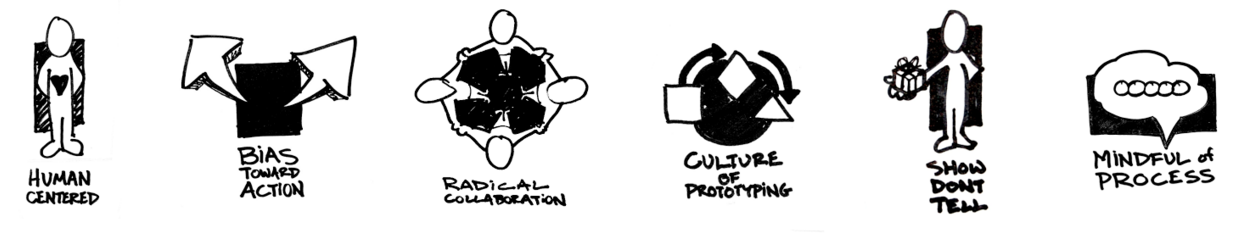
\includegraphics[width=0.9\textwidth]{Figures/ChapterContext/d_mindset}
  \caption[The Mindset of Design-Thinking]{© Hasso Plattner Institute of Design, Stanford University}
  \label{fig:d_mindset}
\end{figure}

\subsubsection{Space}

Part of the Design Thinking culture is an adaptable team working environment. Most furniture is on wheels and can be moved around once requirements change. Different spaces are available for collaborative working, building, communicating and presenting. Doorley et al. devoted a whole book on the design of creative spaces and view it as a necessity to foster collaboration.\footnote{Doorley, Scott, and Scott Witthoft. Make space: How to set the stage for creative collaboration. John Wiley \& Sons, 2011.}  Larry Leifer sees it as one of the three key factors that "influences the ideation and creative energy and output the most"\footnote{Leifer, Larry J, and Martin Steinert. "Dancing with ambiguity: Causality behavior, design thinking, and triple-loop-learning." Information, Knowledge, Systems Management 10.1 (2011): 151-173.}, the other two being absence of a fixed process and an overarching institutional practice of letting change happen. He states that it "lowers hierarchical boundaries, enhances ideation and creativity, fosters and accelerates prototyping and generally increases the rate of learning and change" (ibid.).

\subsubsection{Multidisciplinary Teams}

Brown et al. argue that "to achieve divergent thinking, it is important to have a diverse group of people involved in the process"\footnote{Brown, Tim, and Jocelyn Wyatt. "Design thinking for social innovation." (2010).}. A view that is also supported by Fay et al., who state that organisations more frequently rely on multidisciplinary teams as the increased complexity of tasks requires a wide breadth of knowledge, skills and abilities\footnote{Fay, Doris et al. "Getting the most out of multidisciplinary teams: A multi-sample study of team innovation in health care." Journal of Occupational and Organizational Psychology 79.4 (2006): 553-567.}. This view holds that diversity will lead to an increase in the variety of perspectives and approaches and hence lead to greater creativity and quality of team performance\footnote{Mannix, Elizabeth, and Margaret A Neale. "What differences make a difference? The promise and reality of diverse teams in organizations." Psychological science in the public interest 6.2 (2005): 31-55.}.

\subsection{ME310/SUGAR}

The nine-month graduate level engineering course ME310 has been created over forty years ago at Stanford University and aims to provide engineering students with real-life engineering challenges. The name is derived from the course labelling scheme at Stanford and is short for Mechanical Engineering 310.

Over time, the course evolved to reflect the characteristics of today’s business environment, such as remote, intercultural collaboration, industry alliances, and services orientation.  It has grown beyond the hedges of Stanford University and is currently taught at over twenty universities spread across five continents . This global innovation network is known by the name SUGAR\footnote{Sugar Network - http://sugar-network.org }. The course is now focused on teaching students the innovation methods and processes required for designers, engineers and project managers of the future\footnote{Carleton, T, and L Leifer. "Stanford’s ME310 course as an evolution of engineering design." Proceedings of the 19th CIRP Design Conference–Competitive Design 31 Mar. 2009.}. Therefore student teams work on innovation challenges posed by corporate partners over a duration of nine months. Throughout the projects, students traverse an intense and iterative process of discovering problems and designing and testing various solutions in order to develop a functioning proof-of-concept prototype. The different phases involve need-finding, ideation, rapid prototyping and testing. The course uses Design Thinking to facilitate the human-centred design process. An approach has been recognised as essential for the social acceptance of a solution.

For the duration of each project, each team within the network pairs with another team from a foreign university to jointly solve the proposed design challenge. These partnerships add diversity to the project teams and give students the opportunity to experience true international collaboration, which is an essential skill required in this highly globalised world.

Company involvement provides the reality that is crucial for teams to improve their innovation abilities. In the end, teams deliver functioning prototypes along with in-depth documentation that not only captures the essence of the designs, but also the rationale behind their ideas.

\subsubsection{Project \& Team Setup}

Project teams within ME310 and SUGAR Projects usually consist of two sub-teams from different universities with 3-4 students respectively. The global team comprises participants from various disciplines. This form of interdisciplinary teamwork involves participants working jointly with the objective to find a coherent and holistic end result by analysing, synthesising and harmonising different disciplines. 
The work of each sub-team is facilitated by a dedicated teaching team and project coaches. Often external partner and alumni are invited to coach specific topics, in order to improve communication or to learn how to deal with cultural differences. 

\subsubsection{Process}

\begin{figure}
  \centering
   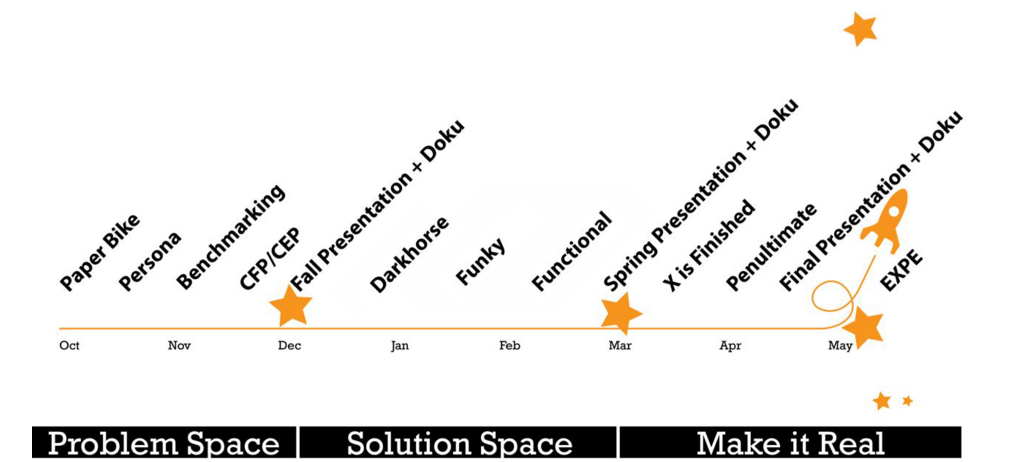
\includegraphics[width=0.9\textwidth]{Figures/ChapterContext/me310_timeline}
   \caption{The ME310-timeline}
  \label{fig:me310_timeline}
\end{figure}

ME310 and SUGAR projects provide a high-level process that rests upon a set of prototypes that define different stages of the design (figure~\ref{fig:me310_timeline}). The course starts with benchmarking and need-finding and continues with the development of exploratory prototypes to foster understanding. The first quarter ending with the autumn presentation and documentation hence mostly considers problem understanding and is defined as the Problem Space. The next quarter focuses on the exploration of the Solution Space, where first parts of the final concept are developed and tested individually. The last quarter, labeled Make it real, serves to integrate the discovered solutions into a complex system prototype.    %Your team, the corporate partner, the project background

%%%%%%%%%%%%%%%%%%%%%%%%%%%%%%%%
% Design Development 
\chapterimage{ChapterImages/DesignDevelopment}
\chapter{Design Development}
\label{sec-development}

% This chapter focuses on benchmarking, needfinding, persona development and how those findings evolved into the first round of critical function and critical experience prototypes. Insights from these prototypes are also discussed.

% Reviewed until Home Status Displays \subsection{Reminder <to be specified>}
% (see additional remark below)

Following our exploration of the smart home and connected car last quarter, the team branched out to a broader design space to dig deeper into compelling technology and customer needs.
\section{Extended Benchmarking}
\label{sec:benchmarking}

During the early benchmarking phase last quarter, we got familiar with the following concepts:

\begin{itemize}
    \item The future of smart cars
    \item Everything that makes up a modern Audi of today
    \item An overview of the current status of smart home technology
    \item Existing connections between home and car
\end{itemize}

\noindent
In summary, we found that smart home technology on the market today offers convenience to users such as the ability to monitor their home from anywhere and remotely control lights from their smart phone, however many users are deterred by the complexity of setup, lack of security, questionable reliability, and obsolescence of such devices. Previous benchmarking details can be found under Appendix \ref{sec:benchmarkingAppendix} and in our fall report.

\subsection{Is 2016 the Year of the Smart Home?}
%As much as 2016 is the year of Linux on the desktop *scnr*

% {Jonathan} Agreed, this is benchmarking. Will move it.
%\todo{Johanna: Not sure if the following subsection belongs here. We did not do needfinding there, it is facts from surveys done by others so rather some kind of benchmarking I would say. If you look at last year's needfinding section it really was compact and short and only summarized all the needs they found in the fall and winter quarter and directly leads on to their final prototype. + This section and the "from needs to prototypes"-section I wrote have some overlaps, we should try and merge that\\
%Dylan: I agree there's some overlap, and I think that's okay. I see from needs to prototypes as being an overall implications of what our results found, and so to me it's okay as is.}

During the last quarter, we mainly explored the technological side of smart homes. This quarter, we were particularly interested in adoption of smart home technology and predictions of future adoption. Despite the technical hurdles to consumer adoption of smart home technology, the belief persists that smart home technology will become ever more ubiquitous. Coldwell Banker conducted a survey of US consumers, and made the following claims:
\begin{itemize}
\item 45\% of users own or will adopt smart home technology in 2016.
\item 70\% of people said buying one smart home product made them want to buy another.
\item The top choices for a home to be considered "smart" were:
    \subitem Locks and alarms (63\%)
    \subitem Temperature (63\%)
    \subitem Light bulbs and lighting systems (58\%)
    \subitem Safety such as fire and CO detectors (56\%)
\item Adopters were slightly more male (57\%) and more likely to be millennials than any other demographic (43\%)
\end{itemize}

\noindent
This defines what has been called the "first wave" of smart home technology. One key distinction for their definition of "smart" is that it includes entertainment systems such as TVs with internet connectivity which are not included in our definition of smart home.

The 2015 State of the Smart Home Report by Icontrol Networks mirrors many of the same findings as the Coldwell Banker report, though adding that "simplicity and ease-of-use trump technological innovation - and today's consumers want devices that solve real, everyday problems" and "right now, most consumers see smart home as a nebulous term without a clear value proposition." This is essentially what our benchmarking and needfinding culminated to last quarter, and has presented significant challenges to our design development. The smart home space offers intriguing features and ample opportunity, but does not address significant latent needs of consumers, yet.

\noindent
Two unique nuggets from the Smart Home Report are:
\begin{itemize}
    \item 72\% of users would sleep better if their parents had smart technology that could alert them if there was a problem.
    \item Insurers are subsidizing and investing in smart technology so that users feel the company is taking a more proactive role in their lives and security, instead of just waiting for an incident to occur. [citation http://fortune.com/2015/12/09/smart-home-insurance/]
\end{itemize}

\noindent
The first point emphasizes security and monitoring as the perceived main driver for smart home adoption. While the primary generation of smart home adopters, millenials, are not as convinced by that need, as their Baby Boomer parents age, the worry about health and safety increases.

The second point offers an interesting avenue to substantially increase smart home technology adoptions, if one was interested in pursuing it. If smart technology can (1) increase the visibility and trust in  companies or (2) reduce potential liability of an incident for insurance companies, then they will be highly motivated to encourage users to adopt smart home technology. Many users do not necessarily have high opinions of their insurance companies, and one representative mentioned that 90\% of users never file a claim, so how can insurance companies still benefit users? This begs the question of how a car company like Audi might benefit users with encouraging adoption of some smart technology that could lower their car insurance premiums such as through more active car monitoring and theft prevention. If our eventual system was able to give users tangible reductions in insurance premiums, both Audi and consumers would be more interested in adopting the technology. And as the Coldwell Banker survey found, having one smart home product makes people want to buy more, so it would also be in the best interest of smart home companies like SmartThings and Wink to encourage any and all adoption of smart home products.

Most of all, users want simplicity and do not want any additional complexity in their lives, even if they have the time, resources, and ability to set up smart devices. They do not want to waste money on products, particularly hardware for their home, if it may be obsolete in a few years. When replacing light switches, one could spend 8X as much for a smart switch that connects to Wink in comparison to a traditional one, but smart technology does not yet offer that much value to consumers. If a system fails, the user may not know how to fix it. One user's convenience is another's inconvenience.

We cannot know for sure if or when smart home technology will become ubiquitous, but we do know that systems that maximize on the user experience and offer significant value to consumers will have the greatest chance at success. Technological innovation for the sake of innovation is not enough to satisfy consumers. So many other aspects of our technologically driven lives are designed with a smooth user experience in mind, and smart home technology cannot be any different. Decades ago, users would put up with pain points in the interface of early email or mobile telephones because of the value it added to their lives, but smart home technology does not currently add such revolutionary capability.

\subsection{Traditional Home Security Systems}

With security being the most important aspect for a smart home, we wanted to get a better understanding of traditional home security systems and their smart home counterparts. Traditionally monitored home security systems have been around for decades through companies such as ADT and Brinks. Users have sensors, control panels, cameras, etc. professionally installed, and then pay a subscription to have a company monitor their home and contact the authorities if the alarm is triggered. Users manually arm system upon departure by pressing a button on the keypad, and must enter a code upon arrival home within a short time to avoid activating alarm. 

\begin{figure}[ht]
\centering
	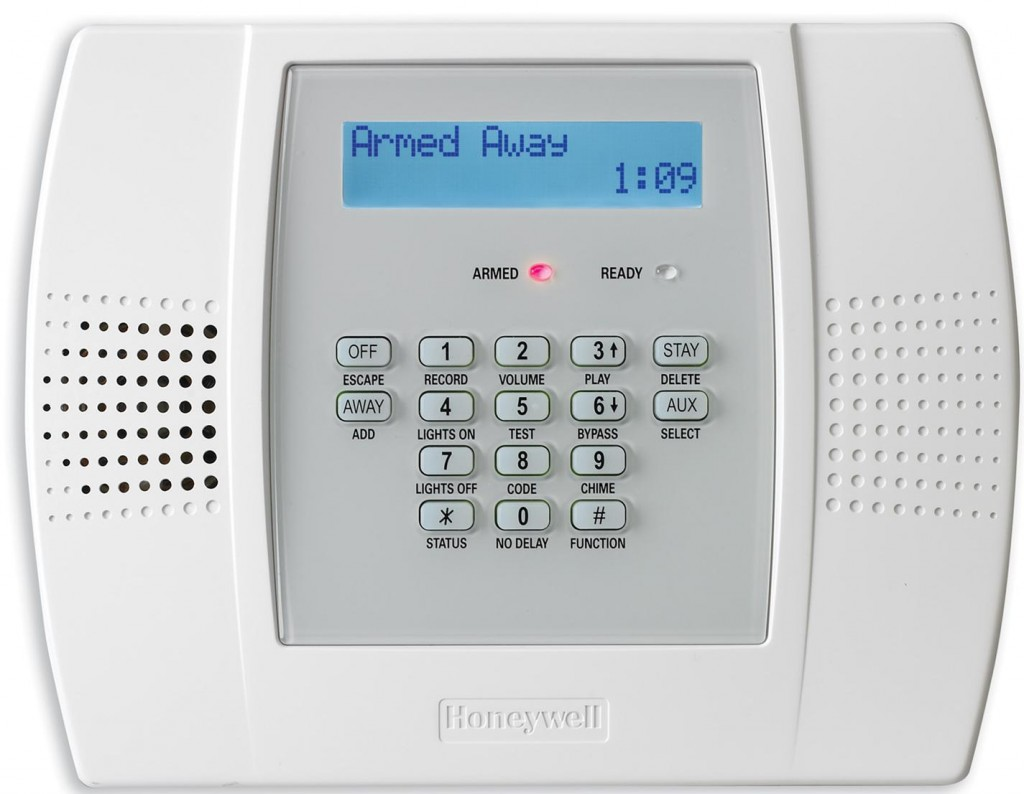
\includegraphics[keepaspectratio, width=4in]{Figures/Benchmarking/keypad.jpg}
	\caption{Sample traditional home security interface. Users must enter code in order to disarm system to avoid false alarm. \protect\footnotemark}
	\label{fig:keypad.jpg}
\end{figure}

\footnotetext{Taken from \url{http://zionssecurity.com/faq-security/the-top-15-questions-about-adt-home-security-systems/} on March 17th 2016}

One noticeable problem with such systems is false alarms, which cost the US economy an estimated \$1.8 billion per year \cite{Blackstone2007}. Users may forget to disable the security system upon entry, or it may be inadvertently set off by babysitters, housekeepers, or pets. Users may be fined for each incident that police unnecessarily respond to, with rising fees for each incident in the same year \cite{Blackstone2007}. Consequently, some users report owning and paying for systems but not often turning them on, to avoid the worry of false alarms. This leaves the home at risk for break-ins.

Of more recent evolution is the idea of full home security and automation, primarily motivated by cable companies trying to shift into another market as traditional cable subscriptions wane. Companies like Comcast, Time Warner, and AT\&{}T offer customers the option to have security systems installed and monitored along with what would be considered the first wave of smart home technology: lights, thermostats, and cameras that can be monitored from anywhere with an Internet connection. Traditional home security companies are now in this space as well, offering higher levels of home automation than before. The advantage of these systems is that they are set up by professionals, avoiding the large complex learning curve that limits adoption of existing add-on smart home technology.

More advanced home security systems today offer users the ability to monitor cameras in the home remotely and arm and disarm the security system at a distance with an additional key fob. In interviews with users, we found that they do not often use the remote monitoring feature, assuming that if there's a problem, the alarm will go off.

Remote key fob disarming presents serious security risks, even with encrypted rolling code sequences. Car thefts occur every year because thieves capture codes when users are parked and lock or unlock their cars. In 2015, a serious flaw in the security of car smart key systems, including Audi/VW, was published by Samy Kamkar \cite[pp. 58 -- 67]{CarKeyHack}.
%\todo{Jonathan: I discovered another hack that sounds simpler. Hope you're ok with it? It's also referenced in the article you provided a link to. Also, I think there's no need to go into too much detail here. Cars can be hacked using their key fobs as a message should be enough.
Potential hackers could intercept the transmission between a user's key fob and car twice, reducing the potential billions of codes down to approximately 200,000, small enough that the code could be guessed by a computer within half an hour.

This could be accomplished using inexpensive and readily available hardware. If the same technology is used in homes, they would be at greater risk as they are stationary, while cars are mobile. A thief could hide electronics to capture wireless codes in the home owner's front entryway, capturing the necessary information to prepare for a future break-in.
%\todo{Jonathan: Same as above, this section should not be concerned with our idea yet
As such, we must be mindful of the potential hackability of our system in the future.
%\todo{Jonathan: I think the citation of the car hack I provided above is a bit better since it is a lot simpler for users of the exploit} - all great, thanks - DJM
%[citation http://www.dailymail.co.uk/sciencetech/article-3201564/Hackers-reveal-flaw-100-cars-kept-secret-Volkwagen-TWO-YEARS-Bug-used-unlock-Kia-Lamborghini.html]

\subsection{DIY Home Security Systems in Smart Homes}

Security is the primary reason that users are interested in adopting smart home technology \cite{ABIhomeAutomationReport2015}. With the advent of modular and adaptable smart home technology, it has become easier for "do-it-yourself (DIY)" users to set up and monitor their own security systems avoiding the costly installation and subscription fees of traditional home monitoring companies. They offer peace of mind at a reasonable cost. All-in-one systems such as Canary\footnote{Canary Connect, Inc. (\url{https://canary.is})}(\ref{fig:canary.jpg} offer motion detection, cameras, and alarms, and will alert user if trouble is detected, but will not call authorities directly, reducing the response time in the event of a true emergency. As a result, these systems do not necessarily have the same magnitude of trouble with costly false alarms as traditional systems, but also do not deter theft as much as more actively monitored systems. There is an obvious trade-off between functionality and cost. \cite{DIYSecurity}

\begin{figure}[ht]
\centering
	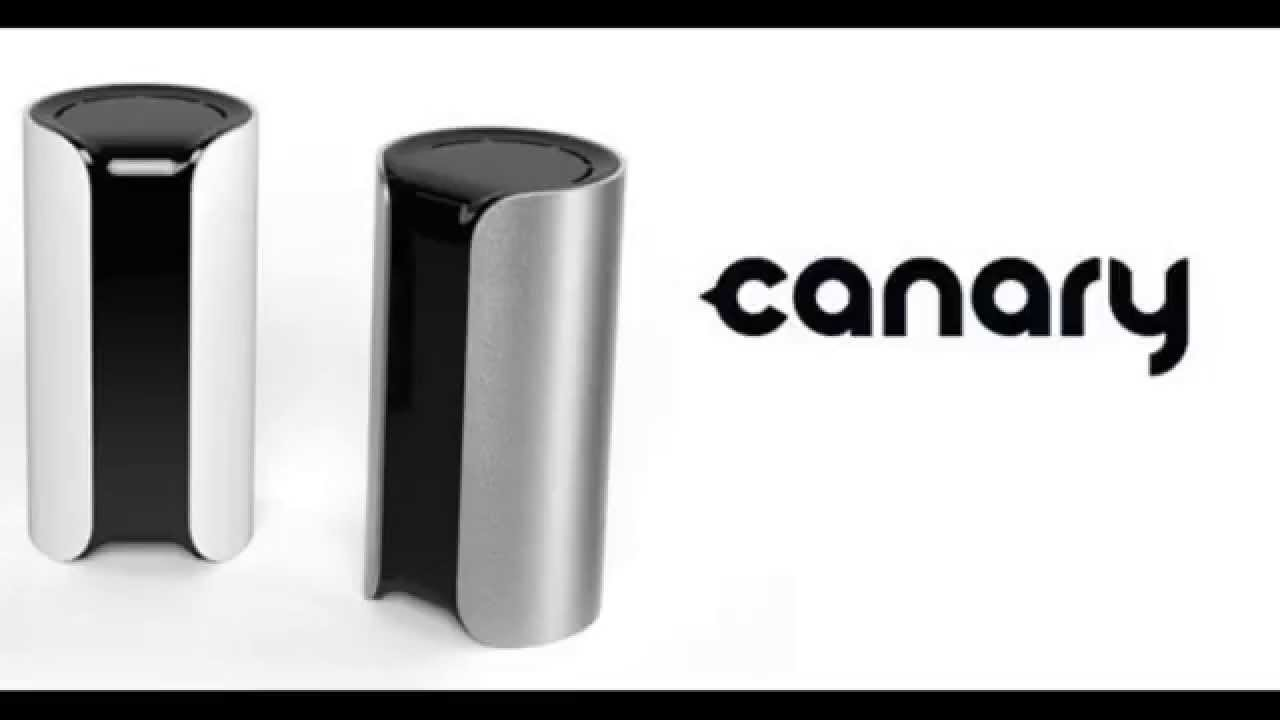
\includegraphics[keepaspectratio, width=6in]{Figures/Benchmarking/canary.jpg}
	\caption{Canary smart home security system allows users to monitor their home from their smart phone. Canary alerts users if significant motion is detected and helps users to contact authorities if intruder is detected. Online storage of video helps users to record and review suspicious moments throughout the day. \protect\footnotemark}
	\label{fig:canary.jpg}
\end{figure}
\footnotetext{Taken from \url{https://www.youtube.com/watch?v=DJUVWkmrqVQ} on March 17th 2016}

\subsection{Smart Locks}

One of the most exciting, but often disappointing, smart home security technologies is the idea of a smart door lock that can be activated remotely with a user's smart phone. This allows one to give temporary "keys" to guests who can let themselves into a user's home using their phone or allow the user to open the front door remotely if there is a package delivery. These locks, such as August\footnote{August Home, Inc. (\url{http://august.com})} (see figure \ref{fig:august.jpg}) advertise the ability to lock and unlock automatically as the user leaves or arrives home. However, the reliability of such systems is questionable, and at least one user we interviewed expressed serious security concerns with such systems. However, another user we interviewed, an architect for high end homes, said that smart locks are becoming quite common in homes, as users want the ability to let others in throughout the day such as babysitters, housekeepers, and mailmen.

Whereas the potential of such systems is exciting, the implementation issues and security risks limit adoption. We can assume that these issues may diminish substantially in the next few years. Moreover, many of the professional home security services described above offer users the ability to remotely lock and unlock their front doors, and as third-party systems become more stable, adoption will likely increase significantly. The last thing users want to do after a long day at work and commute is fumble with their keys in the dark outside their home, and the idea of eliminating that step smooths the user's transition into and away from home significantly.

\begin{figure}[ht]
\centering
	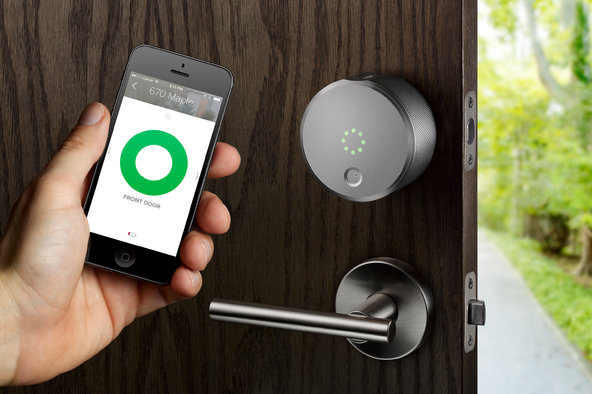
\includegraphics[keepaspectratio, width=6in]{Figures/Benchmarking/august.jpg}
	\caption{August smart lock for the front door can be activated from a user's smart phone. Temporary digital "keys" can be given to visitors so that remote access can be granted while homeowner is away. \protect\footnotemark}
	\label{fig:august.jpg}
\end{figure}
\footnotetext{Taken from \url{http://bits.blogs.nytimes.com/2014/10/14/the-august-smartlock-shows-why-you-should-stick-with-dumb-keys} on March 17th 2016}

\subsection{Home Status Displays} 
%martin
With smart homes having more and more sensors and controllable elements arises the question on how to keep the user in control or convey the status to them. There are several different systems available.

Almost every smart home device or system comes with a smart phone app for control and status functionality. These apps usually have a dashboard-like screen showing the current state of the appliances as well as possibilities to switch devices and configure more complex settings. Figure \ref{fig:wink_relay} shows an example of a smart light bulb control interface. These applications allow users to check on and control the smart home from their phones.

\begin{figure}[ht]
\centering
	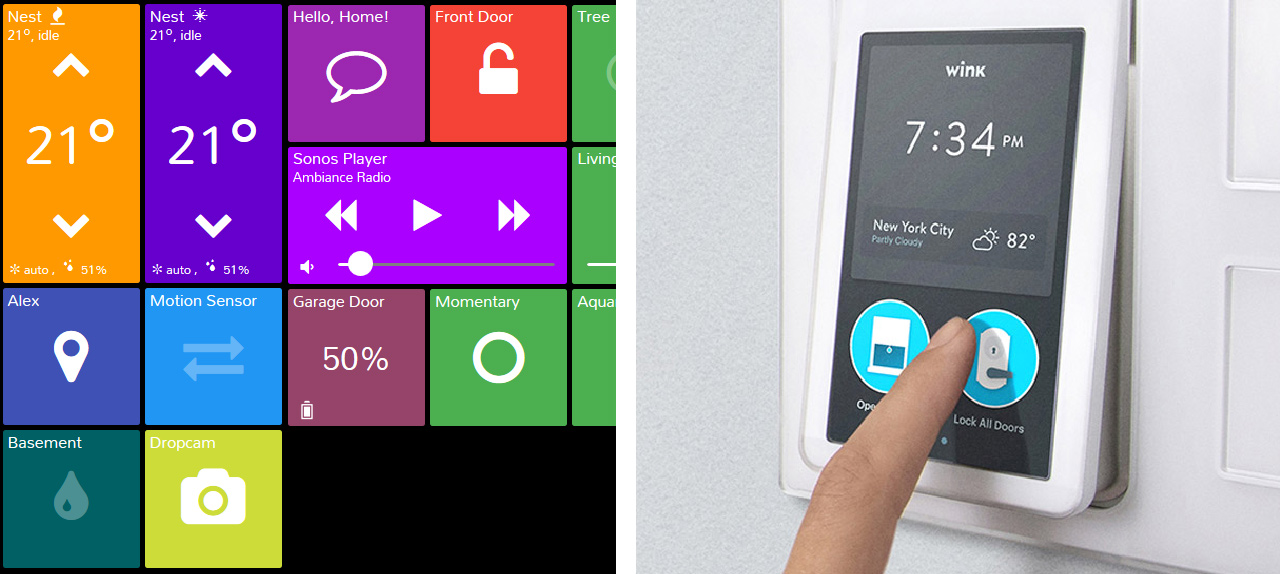
\includegraphics[keepaspectratio, width=6in]{Figures/Benchmarking/wink_smarttiles.jpg}
	\caption{On the left is an example dashboard of the SmartTiles webapp. The image on the right shows the Wink Relay.}
	\label{fig:wink_relay}
\end{figure}

Another category of status displays are bigger dashboards that are installed at a central spot. These usually are dedicated devices for the purpose of interacting with the smart home. Figure \ref{fig:wink_relay} shows the Wink Relay as well as the SmartTiles web app. Both serve as central control and information interface with slightly different approaches. While the Wink Relay uses single purpose hardware the SmartTiles solution relies on existing devices such as tablets or screens that home owners can mount to a wall. These dashboard systems vary widely in features, format, customizability and interaction possibilities.

\begin{figure}[ht]
\centering
	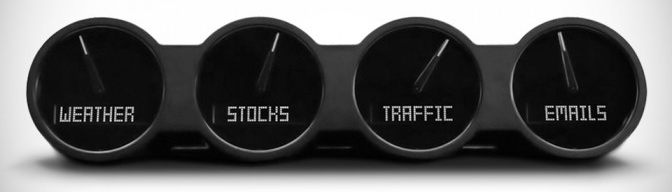
\includegraphics[keepaspectratio, width=5in]{Figures/Benchmarking/quirky_gauge.jpg}
	\caption{The Quirky Nimbus, an analogue gauge displaying various information.\protect\footnotemark}
	\label{fig:quirky_gauge}
\end{figure}

\footnotetext{Taken from \url{http://ecx.images-amazon.com/images/I/41JbtXXjyDL._SY355_.jpg} on March 12th 2016}

\subsection{Reminders and Locators} 
%martin
There are different methods available to aid users not to forget or lose things. Similar to the analog to-do lists there are applications serving the same purpose with added functionality. These apps can notify users by various means (visual, audible, tactile) at specified dates or intervals or when entering or leaving designated areas (geofencing). 

\begin{figure}[ht]
\centering
	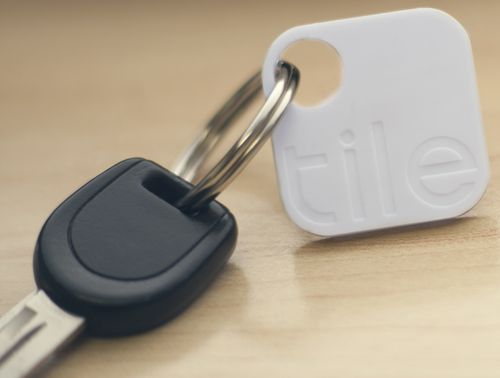
\includegraphics[keepaspectratio, width=3in]{Figures/Benchmarking/Tile_tag.jpg}
	\caption{A Tile bluetooth tag attached to a key.\protect\footnotemark}
	\label{fig:tile}
\end{figure}

\footnotetext{Taken from \url{http://www.rfidjournal.com/lib/x/a/assets/2013/08/Tile_tag.jpg} on March 16th 2016}

With the current Bluetooth Smart (Bluetooth Low Energy) specification a new class of products emerged to aid people locate things. These are small tags that can be attached to important objects. These tags can then be located by means of a smart phone application. The app can determine the distance to the tag up to a range of 30m. Because of the low energy consumption of the radio module, they can run up to a year on a single, small battery. Most tags can also make a noise or vibrate on request from the app. An exemplary product is the Tile tag\cite{tile} displayed in Figure \ref{fig:tile}.

Further applications of this technology include small dedicated buttons that can be attached where the user likes and either are freely programmable or have a fixed purpose.
The Flic smart button\cite{flic} is an example of the first kind, easily programmable by integrating the IFTTT service (for explanation of this see Appendix \ref{text:ifttt}). 
There are more products that add functionality, for example motion, heat and volume sensors into these small buttons like the Sen.se peanuts\cite{peanuts}. These allow the user to add smart features to objects of her everyday life.

Every item users want to be reminded of needs to have a tag attached if it does not have some sort of radio communication itself (e.g. cloth, documents etc.). The Bluetooth tag technology described above is still too expensive and energy consuming for use cases such as sports cloths. There are passive radio-frequency identification tags available which only activate through power delivered from a reader device nearby. These tags can be very cheap and thus can be imagined to be attached to everyday objects\cite{weis2007rfid}. Hsu et al. have described a system that attaches such passive tags to a users items. Based on the users history and calendar information it will then remind her about objects to bring along when leaving his home\cite{hsu2011rfid}.

\subsection{Car Status}
There are a number of ways to get status information about the car from a distance.

The open standard for On-board diagnostics data (OBD) makes a vast veriety of the car's paramaters easily accessible. It has been mandatory to built this into every new car for a number of years. However, it gained widespread popularity only since recently a number of silicon valley tech startups have been using adapters to wirelessly transmit this data to the users' smartphones to generate value for their customers. 

Car manufcaturer have started to make specific functionalities of their models be controllable via smartphone apps. For example, the AudiConnect smartphone app allows users to lock/unlock their car remotely and keep tabs of where the driver parked.

Another example is the Nissan Leaf App which offers a broad set of functionalities like monitoring the battery charge level (Figure~\ref{fig:NissanLeaf1}) and checking on the car's inside temperature as well as adjusting the air conditioning settings (Figure~\ref{fig:NissanLeaf2}).

\begin{figure}[h]
\centering
	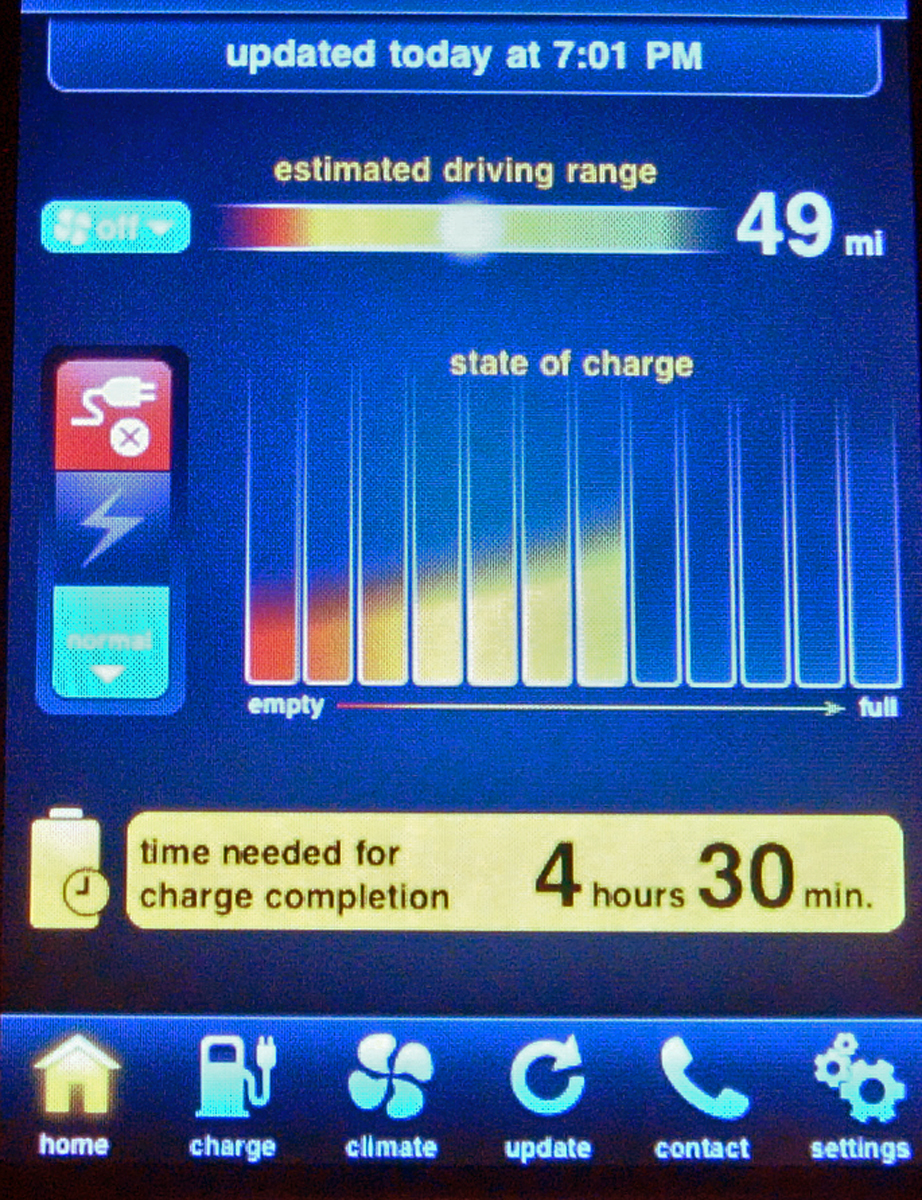
\includegraphics[keepaspectratio, width=3in]{Figures/Nissan_Leaf_mobile_app_battery_status_1733.jpg}
	\caption{Nissan Leaf smart phone app for EV status showing: driving range left, state of charge and time required to complete a full charge.\protect\footnotemark}
	\label{fig:NissanLeaf1}
\end{figure}

\footnotetext{Taken from \url{https://commons.wikimedia.org/wiki/File:Nissan_Leaf_mobile_app_battery_status_1733.jpg} on March 17th 2016 (CC BY-SA 2.0)}

\begin{figure}[h]
\centering
	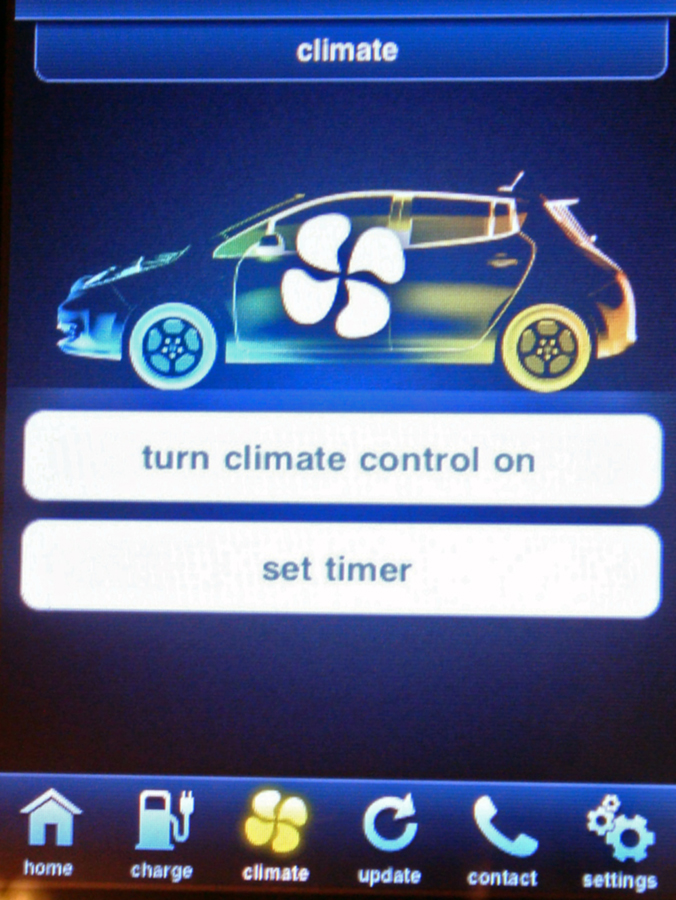
\includegraphics[keepaspectratio, width=3in]{Figures/Nissan_Leaf_mobile_app_climate_control_1713.jpg}
	\caption{Nissan Leaf smart phone app to turn on remotely the climate control.\protect\footnotemark}
	\label{fig:NissanLeaf2}
\end{figure}

\footnotetext{Taken from \url{https://commons.wikimedia.org/wiki/File:Nissan_Leaf_mobile_app_climate_control_1713.jpg} on March 17th 2016 (CC BY-SA 2.0)}

\subsection{Small Modular displays}
%jonas
Since electronic components have become smaller and smaller, certain research groups experimented with the possibilities of very small computers with very small displays.
Siftables (Figure \ref{fig:siftables}) have been designed almost ten years ago. They are small artifacts that can display information and sense certain aspects about their environment. They are connected with other computers through a wireless interface.~\cite{Merrill:2007:STS:1226969.1226984}

\begin{figure}[ht]
\centering
	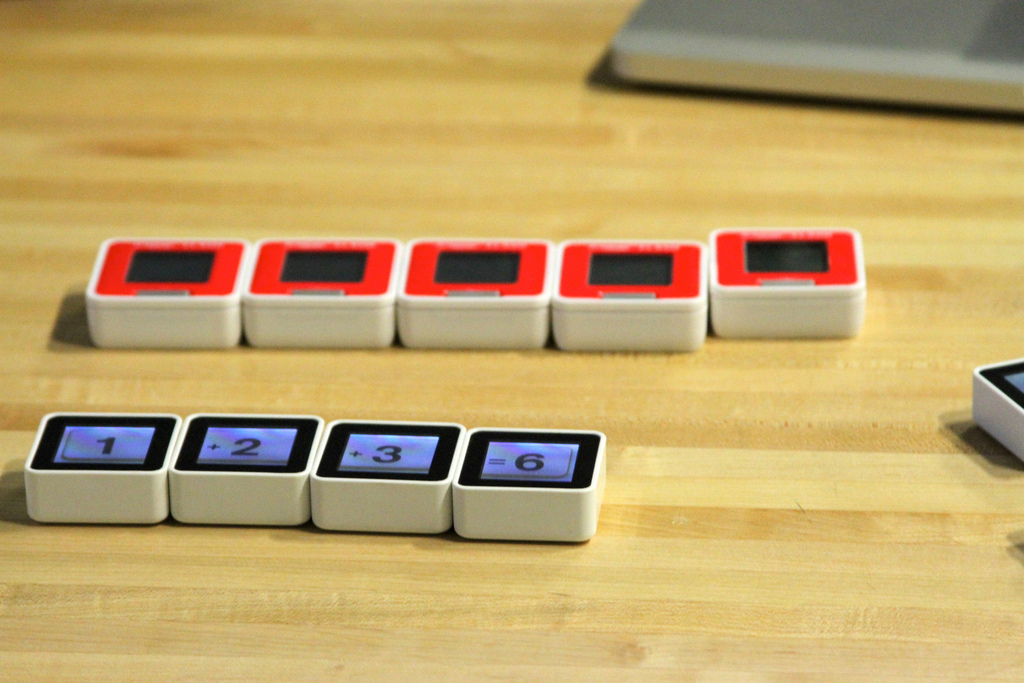
\includegraphics[keepaspectratio, width=6in]{Figures/siftables.jpg}
	\caption{Siftables lined up displaying pieces of information.\protect\footnotemark}
	\label{fig:siftables}
\end{figure}


\footnotetext{Taken from \url{https://www.flickr.com/photos/natematias/6244330415/} on March 12th 2016 (CC BY-SA 2.0)}

After Siftables gained viral popularity online, the company Sifteo was founded and has since then manufactured and sold so-called Sifteo Cubes. After limited financial success of the product, most of its software is now open-source.~\footnote{http://venturebeat.com/2014/12/23/sifteos-intelligent-cubes-go-open-source-after-disappointing-commercial-run/ - accessed  on March 12th 2016}

In 2015 the CloudDrops project (Figure \ref{fig:clouddrops}) followed a similar approach. These devices are supposed to display in particular web-based information and are designed to fit into more diverse architectural scenarios than Siftables.~\cite{Olberding:2015:CSP:2757710.2757718}

The Nimbus by Quirky (Figure \ref{fig:quirky_gauge}) is a recent, but unsuccessful, attempt at displaying basic information through simple displays. This made information available such as weather, travel time to chosen destination given traffic (e.g. work) at any given time. Users found the implementation poor, but did appreciate the desired functionality.

\begin{figure}[ht]
\centering
	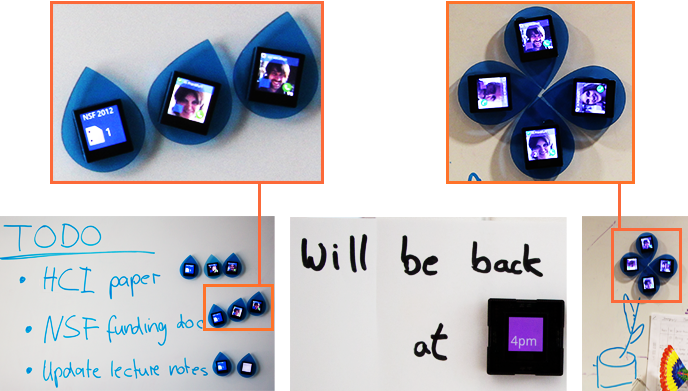
\includegraphics[keepaspectratio, width=6in]{Figures/clouddrops.png}
	\caption{Clouddrops in different usage scenarios.\protect\footnotemark}
	\label{fig:clouddrops}
\end{figure}

\footnotetext{Taken from \url{https://embodied.mpi-inf.mpg.de/research/clouddrops/} on March 12th 2016}

For certain applications, Electronic Paper technology could be an interesting choice --- Especially when displays are supposed to survive long stretches of time without being charged. Small displays using this technology are available at a pricepoint around \$33.~\protect\footnote{https://www.adafruit.com/products/1347 - accessed on March 12th 2016}.

\clearpage{} 

\section{Needfinding}
\label{sec:needfinding}

Need finding was already mostly completed during last quarter. For this quarter, we found out more about Audi owners and visited a truly smart home and talked with its owner.

\subsection{More on Audi Owners}

Upon interviewing additional users this quarter, a key driver for Audi owners became apparent: understated elegance. One well-off Audi owner, who has had 9 or 10 Audis in his lifetime, buys them because they are well-designed, practical (e.g. 4WD standard), and not as pretentious as BMW. This sentiment is mirrored in the Audi TV spot "Performance with the Right Attitude"~\cite{AudiTVSpotAttitude}. Audi owners love the experience of driving an Audi, and even with the recent emissions scandal, one Audi owner said that the Facebook ads to join class action lawsuits against VW were met with comment after comment in defense of the Audi brand and experience. One woman said that she will never buy another car, because she is not sure if she'll be able to buy another Audi diesel, and loves it so much she would never want to get rid of it. While Audi matches the performance of many other luxury cars, it does not accompany performance with cache or arrogance, and that image is appealing to many owners.

Not many Audi owners we interviewed were interested in the technological aspects of the car, let alone the smart home. Though one user did say he bought an A7 because it was the most technologically advanced at the time, but considers himself "technologically compromised" and does not use as many of the features as he expected. He finds the Audi interface a bit confusing, and the setup cumbersome, as did several other luxury car owners we spoke with.

\todo{\{Jonathan\}My hunch is that this use case is too niche and the we should leave this part out}
One unique use case that arose out of these interviews was the case of second home ownership. If someone is fortunate to own a second home and divide their time between two homes, there are unique needs that could be addressed. For instance, one couple lives in 2 homes and owns a total of 3 cars, and has to carry around different keys for each at any given time. If there was a unique system that allowed them to carry around a single key fob for all homes and cars, they would be very interested in that. However, that also brought up the security issue if someone did lose a key fob, it could be used to get into some of the most valuable aspects of their lives, so there would need to be ample safeguards for that. Also, one would still need basic keys for valet parking, housekeepers, etc. There is potential in unifying home and car keys for multiple cars and homes into one incredibly secure device, perhaps as an addition to the smart phone, that can be easily tracked and disabled if misplaced or stolen, due to its importance and value.

\subsection{Visiting a True Smart Home}

One user that we visited, Jack, owns a home that is wired with Control 4 lighting and media throughout the home. This allows Jack to preset certain actions on the switches, such as briefly turning on a series of lights for his daughter to get to her room at night. He has over 20 different events that are programmed. However, we found that he is the only person in his family who is familiar with the system and is comfortable using it.

Jack also owns a home security system, but seldom uses it, as he only has 20 seconds to disarm it upon arrival at home, and the false positives, as mentioned above, are more trouble than it's worth. However such a system does lower his insurance premium, which is a primary reason to keep it. That and on vacations, they can know that the house is secured.

\todo{\{Jonathan\} I don't think this is about the interface. 20 seconds is just too short.}
This visit uncovered the need for more streamlined interface with a homeowner's security system. Similar sentiments have been echoed by other user interviews as well. At the same time, this visit confirmed our earlier suspicions about the complexity of smart home setup and use.

\section{From Needs to Prototypes} %Once the development of prototypes is done, this section could be interwoven with that material.

In designing a system for Audi owners, we must keep in mind that it must be simple, easy to set up (or include setup with purchase) and not too much add additional complexity. From both our interviews and consumer surveys on smart homes, it is apparent that innovation for the sake of innovation is a necessary but not sufficient condition for smart home technology adoption, and our system should not just be another gizmo that can be patched into existing systems. It therefore has to address an underlying problem, anxiety, or need of Audi users.

The basis for every prototype we built and will build are the needs of our actual users. In order to find out about these needs we conducted a series of interviews with potential users and used our findings and insights from testing prototypes to iterate those needs or even discover new needs. This section will give an overview over the needs we identified when it comes to the car, the house or the transition between both.The set of needs we focused on for our resulting problem statement will be presented as well.

We interviewed a great variety of potential users, including Audi owners, families and smart home users and identified multiple basic needs when it comes to using technology in general as well as smart home technology in particular. One of them is simplicity: Users reported that they connect current smart home technologies with cumbersome setup processes and a lack of standards. Instead, they want them to be easy to setup, to integrate seamlessly into their existing technological ecosystem and to function reliably. Similarly, some report that they feel current car technology is too complex for them, resulting in many users not making use of their many in-car features. They demand a more user-friendly interface. This includes multiple users explicitly stating that they prefer a physical interface like buttons over "just another app".

Security is a great concern of many users. Especially when it comes to smart home technology, many were worried about the fact that their house has a lot of dense and very private information about them. Moreover, many feared that a smart home would be vulnerable to attacks. Their requirement for any system being part of a smart home would thus be absolute data security and also privacy. On the other hand, many can imagine to use smart home technology to make their house more secure while they are gone, monitoring things such as the entrance door or windows. 

Especially when it comes to the car but also when asked about the transition from car to house and vice versa, people value a certain comfort and convenience factor and enjoy entertainment. Especially Audi drivers even expect a certain level of comfort - their car is often a status symbol for them and as such it has to be well-manufactured, using only the best materials. 

Another need people often verbalized was freedom and flexibility. They valued the freedom that owning a car gave them such as being able to get anywhere at any time without being bound to things like the public transport schedule or having to book tickets many weeks in advance. In their car they are free to do whatever they want to unlike in most other spaces nowadays - whether it is listening to loud music, singing or sleeping. Their car also allows them to be more flexible, for example when it comes to heavy or bulky baggage such as sports equipment which would not be easily transportable with public transportation without prior planning. In consequence, one important need when it comes to smart homes would be for many that it the technology used is flexible and adapts to their routines without them needing to adjust settings themselves every time they deviate from their normal daily routine. 

While users do want their technologies to be smart to a certain level and adapt to their behavior automatically to ensure flexibility, they also want to maintain some level of control. This also applies to areas like autonomous vehicles where Audi drivers in particular reported that they actually really enjoy the act of driving and would not even want to own an autonomous car since it takes away too much of their control. 

By incorporating these basic needs into multiple prototypes we were able to identify more specific needs when it comes to the transition between the home and the car and vice versa. One major pain users had was carrying heavy things from their car into their house. The biggest use case here was the weekly grocery shopping that can become very heavy very fast especially with families. But also other daily or onetime activities that include carrying heavy things from the car to the house or the other way around such as garden work or vacations were mentioned as pain points that hamper the car-home-transition.

Another pain point we found for both, daily as well as exceptional or onetime activities, is that there is a loss of information in the transition space of home and car. This loss of information can roughly take on three different forms: Information about the home, information about the car and information about things you need to pack and carry between the car and the home. Many people we interviewed tend to forget certain things when they leave the house, among which are their smart phone, their keys or things like sports clothes (see also Figure \ref{fig:testerathome}). Furthermore, many users want to know about their home's current status right before or after leaving the house. Examples here are information about whether all of the windows are closed or whether the heater and all of the lights are turned off. The counterpart is information about the car that they want to know about just after returning home or while they are at home. Such things could be knowing whether the car is safe and locked correctly, knowledge about the car's current maintenance status or gas level or whether the windows are icy and maybe need cleaning before the car can be used. All of this information or rather the lack of this information can hamper the transition or the connection between car and home. More details on the prototypes these needs stem from can be found in the appendix (cf. appendix \ref{sec:PreviousPrototypes}). 

\begin{figure}[ht]
\todo{This just sounds wrong}
\centering
	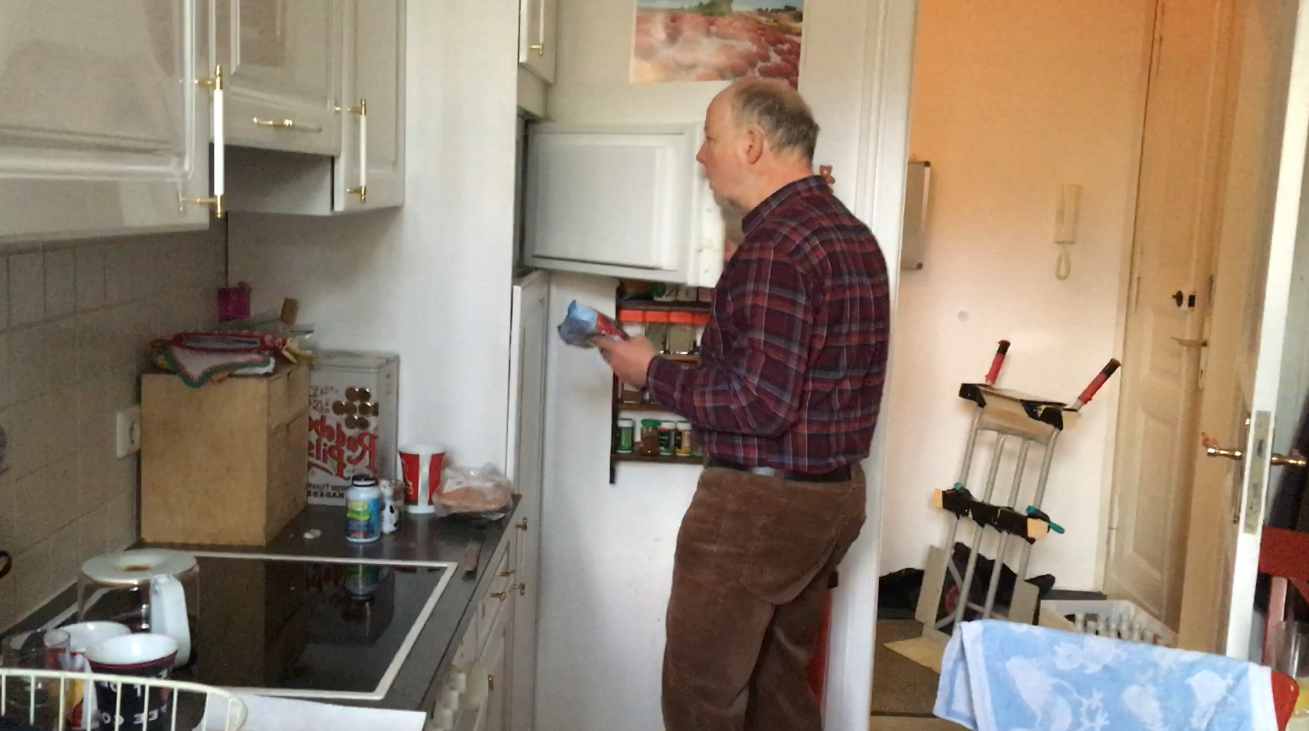
\includegraphics[keepaspectratio, width=\textwidth]{Figures/Needfinding/TesterAtHome}
	\caption{Tester checking whether everything is there}
	\label{fig:testerathome}
\end{figure}


 

\section{Persona}
\label{sec:persona}

As result of our needfinding, we came up with a unified persona encapsulating our insights and identified needs that we focus on in the following chapters. A picture of our persona can be found in figure \ref{fig:persona}.

%{Jonathan} Not nesseary here yet and confusing
%In 3-5 years, 
Linda Becker is 35 years old. She is a senior developer, married and has a 10 year old daughter. They own an Audi A3 sedan and a Q7 SUV which they both share depending on what they need the car for. This also means that they sometimes have communication problems about the state of the different cars if Linda takes a car that her husband had taken before her. For example she sometimes wonders about the gas level if she cannot immediately ask her husband about it. This is important for her so she can plan to gas up the car. Other examples for such problems are icy windows or important maintenance that need to be planned into the schedule as well. Her husband is more often worried about the safety of the car, for example whether it was locked correctly. He would like to have a possibility to check this from home instead of having to walk to the car to check it since they cannot always park the car close to their home.

\todo{Jonathan: City apartment and alarm system? Doesn't sound realistic.}
Linda and her family own a city apartment on the third floor of a high-class apartment building containing many smart home technologies such as remotely controllable windows, lights and heating, smart kitchen appliances and smart media devices. Their house is also equipped with a security system that needs to be armed and disarmed every time the last person leaves the house respectively the first person enters it. Arming the system when leaving the house means that Linda has to be sure whether the house is in a secure state and thus ready to be armed. The smart home technologies in their house do help her to control many things influencing this state, but they are not automated yet since Linda and her husband want to maintain a certain level of control over their house instead of full automatization. However, this also means that she often has to do a second check of the house before she leaves to be sure everything is secure and ready to be left - for example whether the lights are off and the windows are closed. This costs her valuable time. 

% source of persona pdf is in onedrive - missions - winter documentation - PrototypeOverview.pptx 
\begin{figure}
\centering
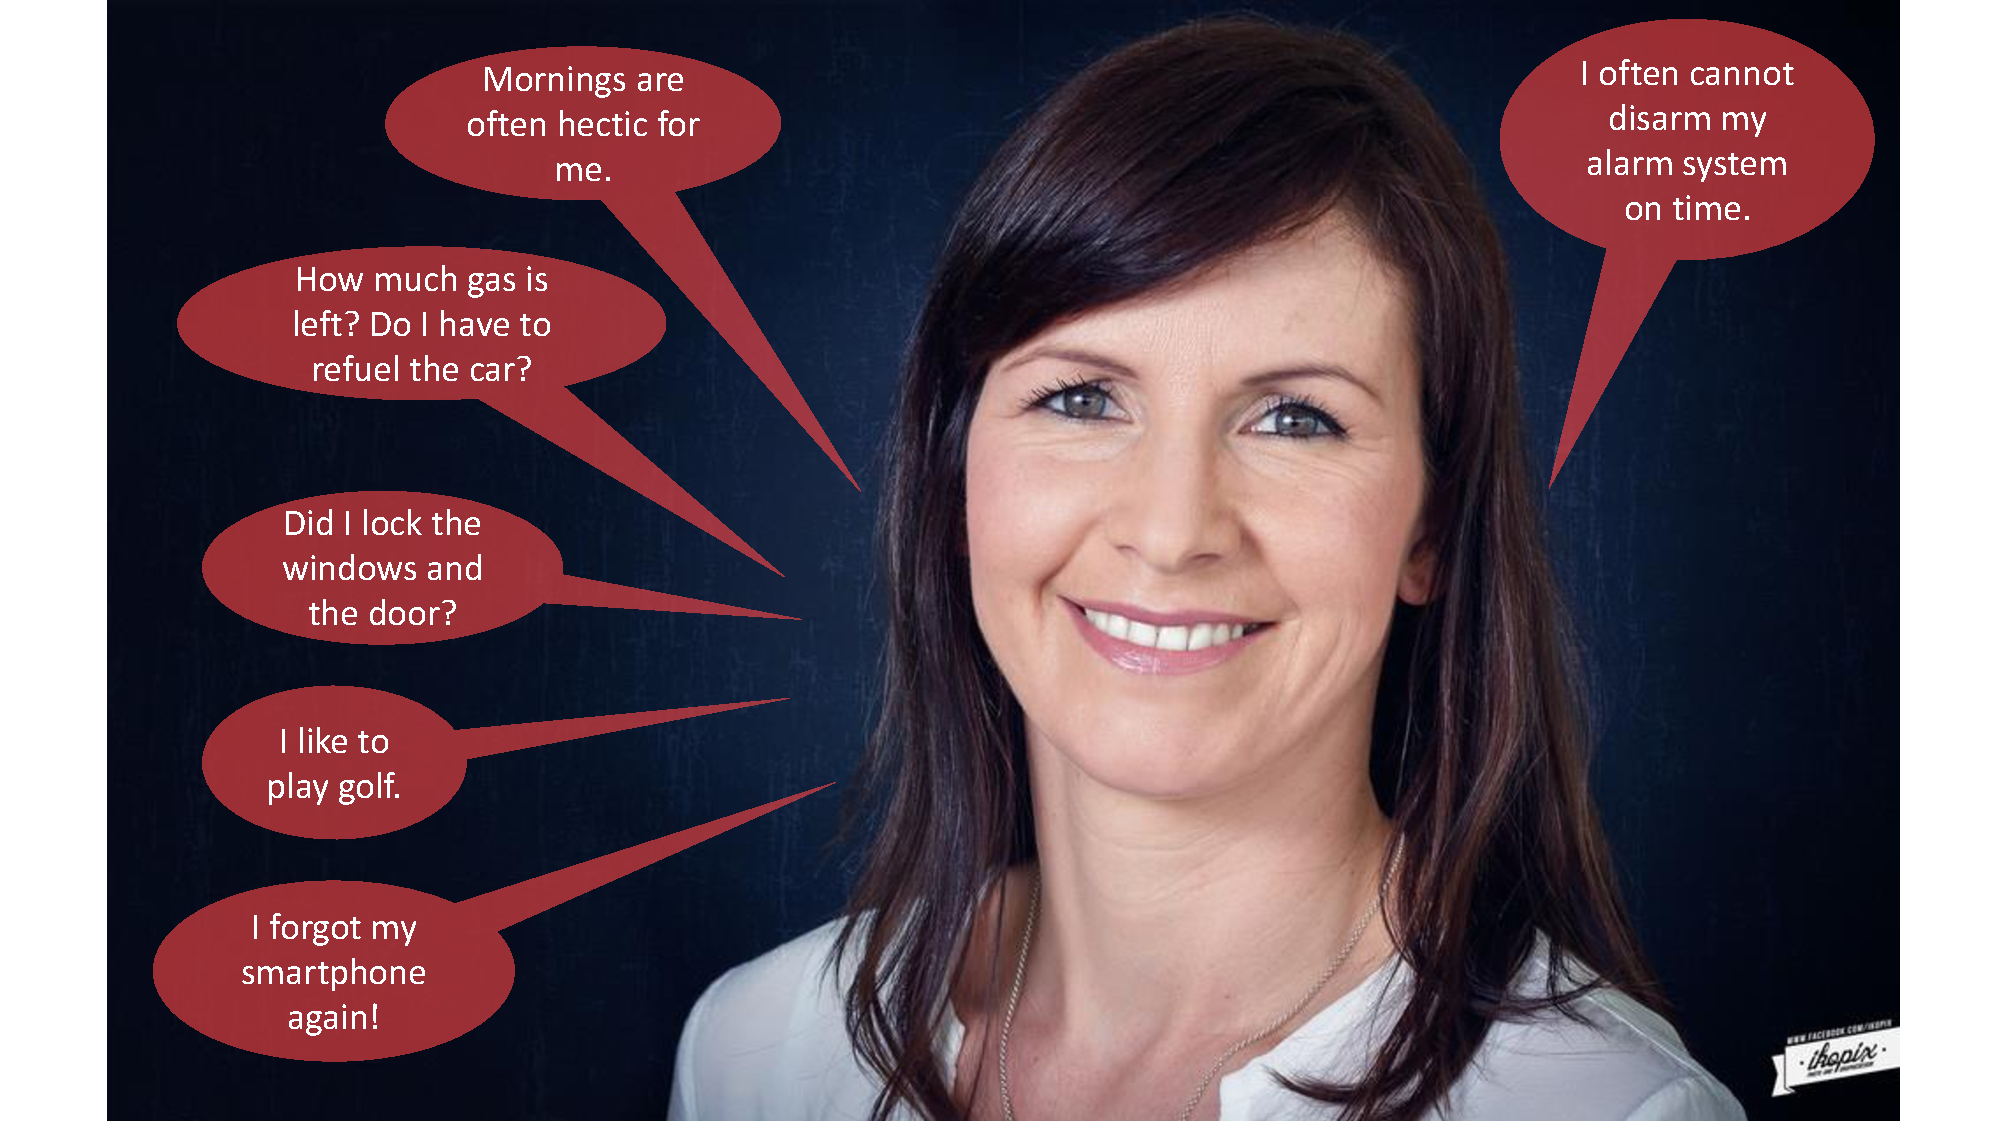
\includegraphics[keepaspectratio, width=5.5in]{Figures/Needfinding/Persona_Linda}
	\caption{Persona Linda Becker\protect\footnotemark}
	\label{fig:persona}
\end{figure}

\footnotetext{Taken from \url{http://www.flickr.com/photos/96071098@N06/17244109369} on March 15th 2016 (license: \url{https://creativecommons.org/licenses/by-nc-sa/2.0/)}}

Disarming the system is similarly painful since it requires Linda to input a code into a panel next to the door. She has to do so within 30 seconds, otherwise the alarm will go off. This happens more frequently to her because she often has her hands packed full with her purse, her daughter's school bag and newly bought groceries when she comes home. This is very annoying and a big pain point for her since it causes extra work and keeps her from really arriving at home and having some time to catch a breath after a long day at work.

Because both Linda and her husband have jobs with high responsibilities and her daughter has to go to school, the mornings with them are often hectic. Many things need to be done and organized such as preparing breakfast, doing housework, packing bags and planning the day for the family. This causes Linda to have to remember a lot of things each day and in consequence she frequently forgets to take everything with her that she needs when she leaves the house. She frequently forgets her smart phone or the charger for her laptop and only notices it when she is already in the car or even at work which can be very frustrating and costs her a lot of time. Also, she likes to play golf now and then for which she always has to pack her sports bag. This sports bag contains many items she needs among which are multiple things she has in her normal workday bag too so she has to repack the bags whenever she goes to sports. In consequence and in combination with her full and hectic days, she does not always remember to pack everything which again is frustrating and time-consuming in the end.

\section{Problem Statement}
\label{sec:problem}

During our exploration of the different ways a connection between smart home and connected cars would make sense, we discovered that there are multiple areas for this:

\begin{figure}[ht]
	\centering
	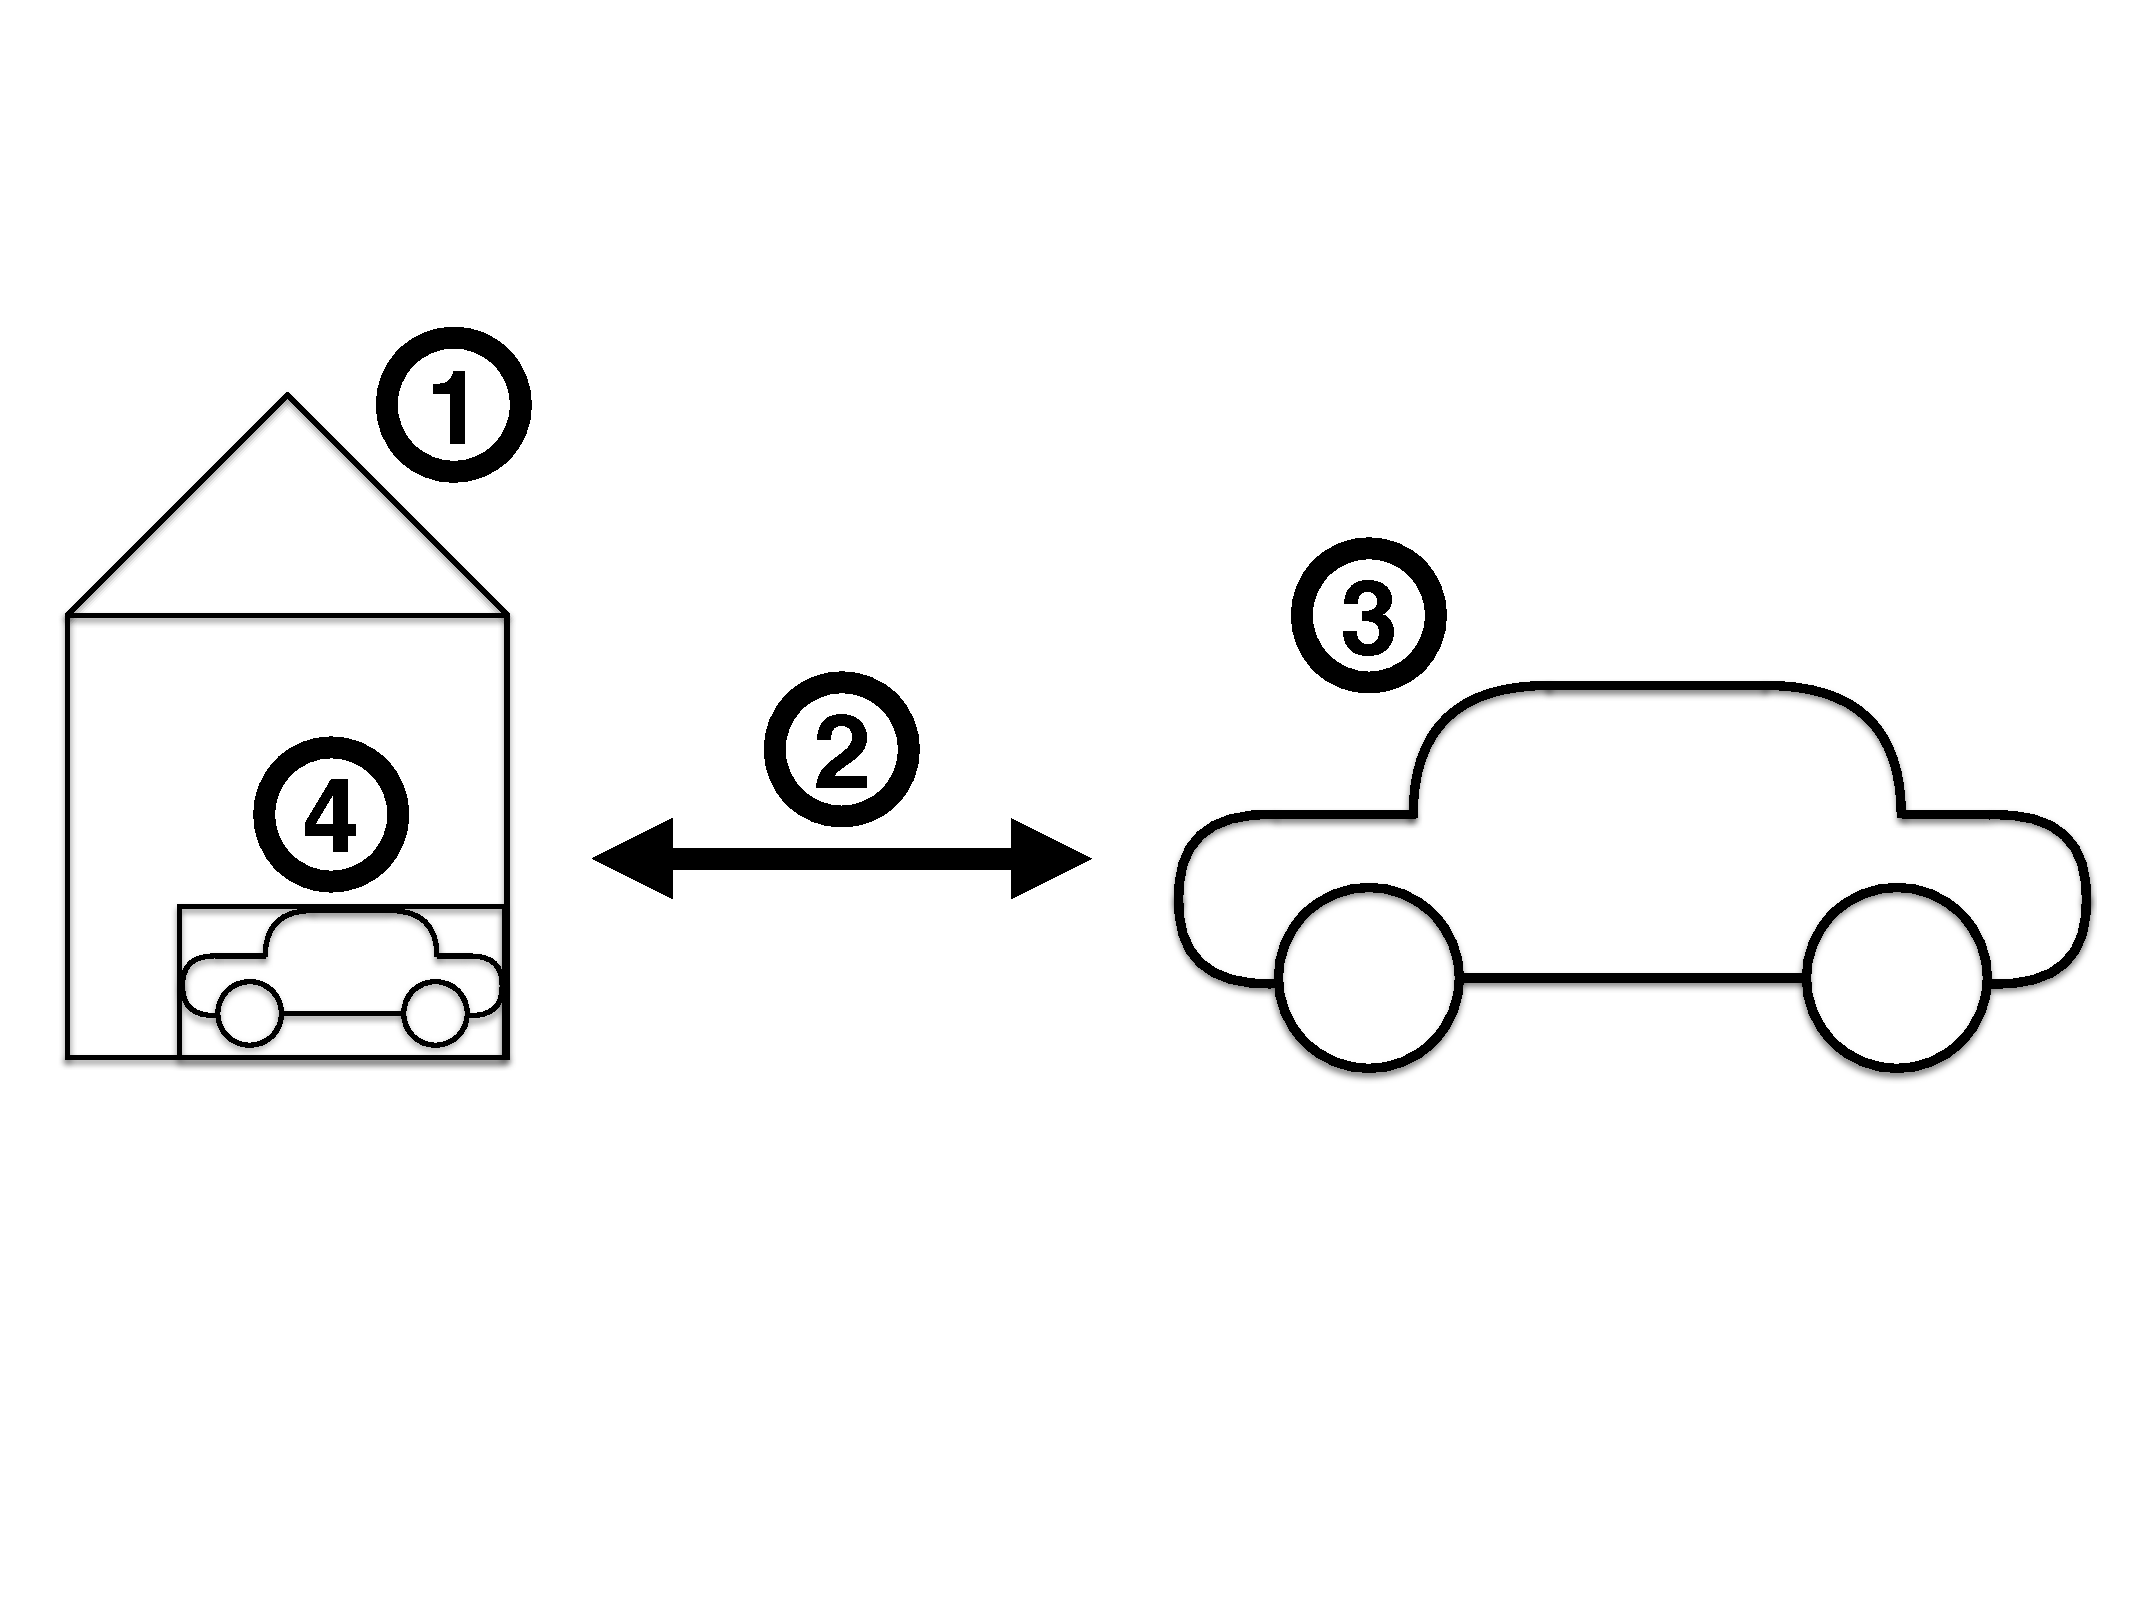
\includegraphics[width=\textwidth]{Figures/Development/CarAndHomeEquals}
	\caption{The four areas we identified for the combination of smart home and connected car}
	\label{fig:CarAndHome}
\end{figure}

\noindent
\\\textbf{1. Accessing the connected car from the smart home}
\\A subset of Audi owners take great pride in their ownership and therefore want to display that. They want the physical presence of the Audi brand to show their prestige, which also accounts for why most car manufacturers still design a heavy key fob even though technically it is not necessary to do so. When people leave their car, how could we still create an Audi ownership presence at home? It could be a physical product fixed at home, or a portable device that the user carries with them, or even some virtual products embedded in the user's cell phone or smart home system.

\noindent
\\\textbf{2. The transition between home and car}
% {Jonathan} This does not really make the case strong for the transition between home and car since entertainment is a mere luxury. Needs to be rewritten
%\\Car and home are two of the places where people spend most of their time (the third being their workplace), yet there are few connections between those two. People transit between car and home several times per day but the experience is not smooth enough. What if the home knew what the user was listening to on the radio before arriving home and turned on the home entertainment system when they walked in the door?


\noindent
\\\textbf{3. Accessing the smart home from the connected car}
\\There are a large number of people who spend hours in their cars everyday. For those, some technology that can improve their experience in traffic or on their long commute would be highly beneficial. Also, people sit and wait in their car to pick up their child from school or waiting for a client. In these cases, they want to be more productive, for example, reviewing documents for a meeting, checking emails, or messages. And as 
% Audi corrected us to not say autonomous and instead use "piloted"
piloted driving is around the corner, we can expect there would be more demands for in-car activity. Accessing the smart home from the connected car has some merits in these cases. Still, being productive inside a car is something that is less related to smart home in particular but is rather a concept that can be applied to many fields.

People who commute a lot in the car might also be interested in easier communication with families or friends. For example, letting the car tell the stay-at-home partner the expected time the other one would arrive home so that they can prepare dinner. Or the driver might be interested to take a look at what their kids are doing when he is in traffic to make sure they are not up to mischief.

\noindent
\\\textbf{4. The car as part or an extension of the smart home}
\\The car as part or an extension of the smart home is a truly futuristic concept that sees a physical integration between the two areas car and home. \todo{Dylan: This concept was tested in SU's darkhorse, and while interesting, did not seem like a viable approach. Is this something we really want to do? Or am I misinterpreting what is meant by physical integration of these spaces?\\
Jonathan: My understanding was that this part represents four viable areas that we could concentrate on but in the end we show that the transition between car and home is the best in our case}
\\\\
Based on our need finding and the factors mentioned above, we put our problem statement as: \textit{how might we improve the transition between home and car and make the Audi brand more present in the process?}.    %Results of benchmarking, need-finding, CFP, CEP etc.

%%%%%%%%%%%%%%%%%%%%%%%%%%%%%%%%
%MRC5Dec2102 Added Venture Requirements suggestion.
%Design Requirements Chapter
\chapterimage{ChapterImages/Requirements2}
\chapter{Design Requirements}
\label{sec-requirements}

%%%%%%%%%%%%%%%%%%%%%%%%%%%
% \begin{remark} \color{blue}
% % \vspace{-0.3cm}
% {\large What will be required for any solution that is consistent with your current vision and meets your user's needs?}

% In 2013-14 we experimented with omitting Requirements for the Fall Documents. We concluded that it was a mistake -- even preliminary requirements are useful for coming to grips with the problem space.

% Articulating design requirements is a critical task for a team that starts with a broad problem and needs to determine \emph{what to design}. After need-finding, and technical and user benchmarking, the team proposes a {\em class of design solutions} that will fulfill {\em requirements}\, associated with the problem. 
% These requirements are among the first items of value that teams can deliver to sponsors.

% As the design continues, requirements become more concrete and detailed. The direction of the project may change, leading to different kinds of requirements. Typically, new {\em de facto} \, requirements are discovered and documented. 
% Ultimately, competing designs are evaluated with respect to the requirements. If you can't tell whether a design satisfies the requirements, the requirements are too vague!

% In the fall, requirements will be preliminary. Still, it is worthwhile to articulate what you think will be needed, given what you've learned thus far. You might find that the 3-column format (e.g., Table \ref{tab:mediums1}) demands more precision than you have at this stage. 

% The remainder of this section contains sample requirements (not an exhaustive set but enough to give an idea) from Autodesk Fall 2007-08 \cite{Autodesk2008Fall} and Audi Fall 2008-09 \cite{Audi2009Fall}.
% \normalcolor \end{remark}
%%%%%%%%%%%%%%%%%%%%%%%%%%%

\section*{Introduction}

For our system to serve as a desirable and useful connection between car and home, it should fulfill these high-level requirements:

\begin{enumerate}
\item Enhance the experience of arriving home from the car
\item Enhance the experience of leaving home to the car
\item Not add any complexity to a user's routine
\end{enumerate}

\noindent
These requirements are further broken down and elaborated below. Our system AudiSeamless contains two main parts: 
% {Jonathan} bowl less necessary compared with sensor
%a bowl that serves as storage and 
\begin{enumerate}
    \item \textbf{AudiDefender} which is a sensor to detect the user's key fob
    \item \textbf{AudiBits}, small displays showing the user what they forgot
\end{enumerate}
 \noindent The functional requirements for the system as a whole are outlined as well as separate physical requirements for AudiDefender and AudiBits.


\section{Design Requirements for AudiSeamless}

\subsection*{Functional Requirements}

\textcolor{white}{text needed to format tables correctly}

\begin{center}
\tablefirsthead{%
\hline
\textbf{Requirements} & \textbf{Metric} & \textbf{Rationale} \\
\hline}
\tablehead{%
\hline
\multicolumn{3}{|l|}{\textit{\small{continued from previous page}}}\\
\hline
\textbf{Requirements} & \textbf{Metric} & \textbf{Rationale} \\
\hline}
\tabletail{%
\hline
\multicolumn{3}{|l|}{\textit{\small{continued on next page}}}\\
\hline}
\tablelasttail{\hline}
\bottomcaption{Functional requirements for AudiSeamless}
\begin{supertabular}{| p{32mm} | p{50mm} | p{53mm} | }
		\hline Disarm home security system & Time to disarm is less than 5 seconds & Must take less time than existing method of entering code on keypad.\\
		\hline Arm home security system & Time to arm is less than 1 second & Must be equal or less than existing method of pressing single button to arm. Will require separate signal than removing key fob, as user may not want to arm system.\\ 
		\hline Automatic arming of system if user forgets. & System automatically arms system if nobody is home for 15 minutes and user does not arm upon departure. & Users may forget to arm system upon departure (will need second factor - button, etc.) \\ 
		\hline  Detect Security fob at variable distances & Detect security fob within an adjustable range of up to 1 meter. & Users should have flexibility in detection of the key fob. They may want to keep the key fob in a purse or bag, and not explicitly take it out to place it in a particular place. The distance cannot be too large so as to broadcast the signal outside of the user's home, minimizing the risk of hacking into the system. A 1 meter radius would encompass the standard entryway table or shelf that one may store their bag in or keys on.\\ 
        \hline Check status of home alarm system & Interfaces with existing home alarm system to check status of sensors every 0.5 seconds & Must keep apprised of changes in home security status. For the interval, everything below 1 second should be quick enough for a user to recognize the change as ``immediately'' \\
        \hline Consume status of smart home devices & Interface with existing smart home ecosystems such as Wink or SmartThings to detect state of lights, media etc. Update status every 0.5 seconds & Users want a unified interface for their smart home instead of needing to pull out their smart phone app. Rationale for time same as above\\
        \hline Remind user to bring important belongings. & System can detect presence of at least 10 tags that user can place on important items. & From testing, users liked the idea of reminders to bring things. Users also mentioned they would not want more than 10 AudiBits displays (1 display = 1 tag)\\
        \hline \textbf{Jonathan: Do we need this? We did not agree on that feature so far with the team.} Connects with user's calendar to suggest items to bring & System interfaces with Google Calendar to suggest items to bring for specific days or trips. & We would want smart suggestions such as "I see you are going to Lake Tahoe this weekend, and your snow chains are not detected in your car. Would you like to bring them?" \\
        \hline Car alert can be pushed to device. & Interfaces with car systems every 5 seconds to alert user of problems. & User need to know that car is okay at any given time, and if an intrusion is detected, be alerted of it promptly. Active checking may not be technically viable. \\
        \hline Display car status & Display at least 4 main indications of status (away, urgent attention, suggested maintenance, and all okay) & Users expressed interest in making sure their car was okay while it was parked on the street.\\
        \hline Display car driving range & Displays accurate range to within 1/8 of a tank. & Give users an idea of how much driving range they have, but exact mileage is not needed. Accuracy of driving range depends significantly on driving style, road conditions, weather, etc. 1/8 of a tank increments is a standard breakdown of a tank's level in the US.\\
        \hline Alert user of car intrusion & User is alerted of car break-in within 5 seconds of it happening to alert authorities. & We want the user to know immediately if something is wrong with their car so they have the best chance of catching the intruder.\\
        \hline Alert user of maintenance issues & Maintenance signals sent to system every time car is turned on and off. & User should be reminded of maintenance issues when they have the ability to address them (i.e. schedule a time to go to the mechanic or set aside time to look at issue themselves on calendar).\\
        \hline Send indication to car that user is leaving upon departure. & Signal is sent to car within 5 seconds of home system arming or indication given. & Sending signal to car can warm up interior, boot navigation, and connect car to internet before user enters car, based on what the user desires.\\
        \hline Programmable to work with any Audi car or multiple cars. & System interfaces with at least 2 Audi vehicles and can be reprogrammed easily. & Our users may have more than 1 vehicle, and whereas we are not as concerned with interfacing with other brands (we'd like to encourage brand loyalty) \\
        \hline Recharge key fob battery & Recharge existing key fob battery equivalent (CR2032 - 210 mAh, 3V) in under 8 hours & This is the model, capacity, and voltage of existing Audi key fobs, and whereas we could not directly recharge this one, we could install an equivalent battery that could fully recharge overnight.\\
        \hline Resilient to hacking & System cannot be hacked by brute force attack (guessing of wireless security codes) in less than 12 hours. & Security is a common concern with smart home technology, and ours should be secure enough to deter potential intruders that hacking into system isn't worth it.\\
\end{supertabular}
\end{center}

\textcolor{white}{text needed to format tables correctly}

\subsection*{Physical Requirements}

\begin{center}
\tablefirsthead{%
\hline
\textbf{Requirements} & \textbf{Metric} & \textbf{Rationale} \\
\hline}
\tablehead{%
\hline
\multicolumn{3}{|l|}{\textit{\small{continued from previous page}}}\\
\hline
\textbf{Requirements} & \textbf{Metric} & \textbf{Rationale} \\
\hline}
\tabletail{%
\hline
\multicolumn{3}{|l|}{\textit{\small{continued on next page}}}\\
\hline}
\tablelasttail{\hline}
\bottomcaption{Physical requirements for the AudiSeamless Bowl/Sensor}
\begin{supertabular}{| p{32mm} | p{50mm} | p{53mm} | }
		\hline System stores Audi key fob and standard set of keys & Storage area of system is at least 750 cm3 & If users choose to store keys in system, it should be able to fit any standard set of keys including the key fob as well as any other house, storage, work, or miscellaneous keys the user chooses to store.\\
		\hline System is portable. & Weight less than 15 kg & Urban users are more likely to move apartments, so the system should be easily movable from one apartment to the next.\\
		\hline System fits on standard entryway table & Footprint of less than 0.2 m2 & System should be easily placed on a table near the user's front door. \\
		\hline System is durable and robust & Must function for at least 4 years and cannot be significantly altered by an average man or woman applying a full impact force on structural elements of the system & Since Audi is known for reliable and well manufactured cars, any final solution should be in line with this and should be resistant to daily use by an average human and vandalism. The average car lease is 3-4 years, so it should at least last as long as the first owner will likely own the car.\\
		\hline Solution should be safe for children to be around. & There should be no pinch points, sharp points, etc.& Many potential users have children, and we would not want to endanger them.\\
		\hline System should be aesthetically pleasing & At least 80\% of surveyed users should react positively to the device forms & A pleasing system will encourage adoption and use and is in line with the characteristics of the Audi brand.\\
		\hline Subtly incorporate the Audi logo into the design. & Logo is at least 1 x 4 cm visible when walking by the system. & We want to bring the Audi brand into the home so that users can show others their love for the car.\\
\end{supertabular}
\end{center}

\begin{center}
\tablefirsthead{%
\hline
\textbf{Requirements} & \textbf{Metric} & \textbf{Rationale} \\
\hline}
\tablehead{%
\hline
\multicolumn{3}{|l|}{\textit{\small{continued from previous page}}}\\
\hline
\textbf{Requirements} & \textbf{Metric} & \textbf{Rationale} \\
\hline}
\tabletail{%
\hline
\multicolumn{3}{|l|}{\textit{\small{continued on next page}}}\\
\hline}
\tablelasttail{\hline}
\bottomcaption{Physical requirements for the AudiSeamless Modular Display}
\begin{supertabular}{| p{32mm} | p{50mm} | p{53mm} | }
		\hline Battery lifetime has to be sufficiently long. & Must last at least 1 week without need for recharging. & We do not want users to need to constantly recharge their screens.\\
		\hline One AudiBit can be setup via a smart phone app. & An inexperienced user must be able to set up system within 20 minutes. & We want our system to be accessible to a wide range of users.\\
		\hline One AudiBit has to be easily attachable and dettachable to most surfaces within the house (such as walls or the fridge) & Removable adhesive (such as Command Strips) must support at last 500 g of weight. & We cannot have the screen fall off the walls.\\
		\hline One AudiBit has to be sufficiently big enough to display easily visible icons &  Icon must be at least $16 cm^2$ & Visible from at least 2 m away. Exact size estimated from testing.\\
\end{supertabular}
\end{center}

\subsection*{Constraints}
\begin{itemize}

	\item The bandwidth required must not be prohibitive to standard engineering offices. 
	\item The solution has to be consistent with the look, feel, and use of Audi branded products (cf. section 2.3.1.2) 
	\item Users need to feel like they are in control of the system at all times. Few users are very interested in systems acting to anticipate their needs.
	\item Must be able to adapt to the flexible schedule of the user. 
	\item The signals for the security system disarming cannot reach outside of the user's home or apartment, minimizing the risk of burglars capturing signals and disabling the system on command.
	\item If the body of the key fob itself changes, it must fit in the average user's pocket or purse.
	\item Any connection with the car will be powered by the car's internal battery, which will not handle significant sustained power draws. 
\end{itemize}

\subsection*{Opportunities}
\begin{itemize}

    \item Be the first one to offer the "Killer-App" for smart homes that does not seem to exist yet even though people are generally interested in the smart home. 
	\item Design a device that would pay for itself through reduced home or car insurance premiums, improving business case for adoption.
	\item Simplify an automated smart home setup and use through implicit action of walking into the home and depositing the key fob.
	\item Use the same protocol as the smart key system to minimize the need for additional hardware (though we will not be able to easily get access to this for the purposes of the project, so we will emulate the protocol with a similar system).
	\item Smart keys are systems that Audi owners are familiar with and could easily learn to use at home.
	\item As key fobs become more "smart" and as users generally do not place them into car to charge, the power consumption increases, and therefore battery life decreases. There is an opportunity to eliminate the need for users to replace the batteries themselves. 
	\item Several users have not expressed compelling need for an AudiConnect subscription features, but perhaps our system could increase the subscription level of 
	\item Perhaps the screen could be cut into tile work in kitchen or walls so that power could be supplied continuously and it would literally have stronger integration with the house.
	
\end{itemize}

\subsection*{Assumptions} 
\begin{itemize}

    \item Users keep key fob in the same place when they get home.
	\item Users own home security systems of some sort.
	\item Audi owners will own and be comfortable with the basic functionality of smart phones. 
	\item Cell coverage in use area is strong enough to add nearly constant connectivity between car 
and internet/home with at least 3G speed.
	\item Users own and know how to set up and use smart home devices 
	\item People see a benefit in automating things in their home 
	\item Users have AudiConnect credentials, which allow them to interface with the internet and car remotely at the moment.

\end{itemize}


 

%%%%%%%%%%%%%%%%%%%%%%%%%%%%%%%%
\chapterimage{ChapterImages/Requirements}
\chapter{Design Specifications}
%\chapter{Design Description}   %This title will make more sense in Winter and Spring.
\label{design-description}

%%%%%%%%%%%%%%%%
% \begin{remark}\color{blue}
% This \textbf{Design Description} chapter defines what the design is. For fall, it's really your vision or proposal for what you think the design might be by the end of winter or spring quarter. So let's call it the \textbf{Design Vision} in the fall documents. It will be a short chapter. 
% Even so, on the basis of preliminary need-finding, benchmarking and critical function evaluation, you have some idea of what may be appropriate. \emph{Take a point of view and assert it!}  
% \begin{itemize}
% \item A CAD rendering or systems diagram, or schematic, or a concept drawing is appropriate to help explain your vision. 
% \item If you find yourself adding rationale, or discussing design alternatives or how the vision came about, you are writing text that should be moved into the end of the Development section. This is section is about what the design (or vision) is, not how it came to be.
% \end{itemize}
% \normalcolor \end{remark}
%%%%%%%%%%%%%%%%


%\section{Vision}
%\label{vision}
%
%For winter, although you now have a design to describe, you probably want to start off your Design Description chapter with a reminder of the overall vision, toward which your current design is an important intermediate step.
%
%Use this section to describe your vision or proposal for what you think the design might be. Ideally you should have a sketch, a diagram or other images to help define it.  
%\section{Specifications}
%\label{specifications}
%
%In winter and spring here is where you describe what your design is. 
%\begin{itemize}
%\item Define the subsystems and how they go together.
%\item Use diagrams, CAD renderings, tables, etc. to make it clear. 
%\item Use flow charts or pseudocode to describe procedures.
%\item Detailed source code and numerical data should go in an Appendix section or, if really long, on a CD or other electronic format (nobody will wade through the printout).
%\end{itemize}
\vspace{1em}

Several prototypes were built to explore how we might improve the simplicity of interfacing with smart home technology, and how we might improve the transition between home and car. We capitalized on the need for users to (1) enjoy peace of mind about their home and car at all times, given that security is the primary reason users adopt smart home technology, (2) remember important items in their daily routine.
\section{Critical Experience Prototype: Leave-home Button}

For a long time, we have talked about some sort of physical system that is in the house that conveys information about the car and journey ahead to the driver as they are getting ready to leave. We wanted to see what information would be useful to people, and if they would be able to listening to it as they are busy getting ready. So for the critical experience prototype, Stanford team decided to a simple interactive button using the RBBB that the user would press as they are leaving home. This button triggers smart home conditional statements (e.g. turn off lights and lock door behind you) and conveys information about the car and trip ahead (e.g. sending navigation to car, turning on heat). The audio feedback tells users that their command was detected. Useful information would be pushed to user’s phone and car as desired.

We wanted the users to have some kind of distracting activity, mimicking picking up and finding things before they leave the house. People report they are often looking for their wallet, brushing their teeth, etc. So we designed a card sorting task in our experiment to mimic that process.

\begin{figure}
\centering
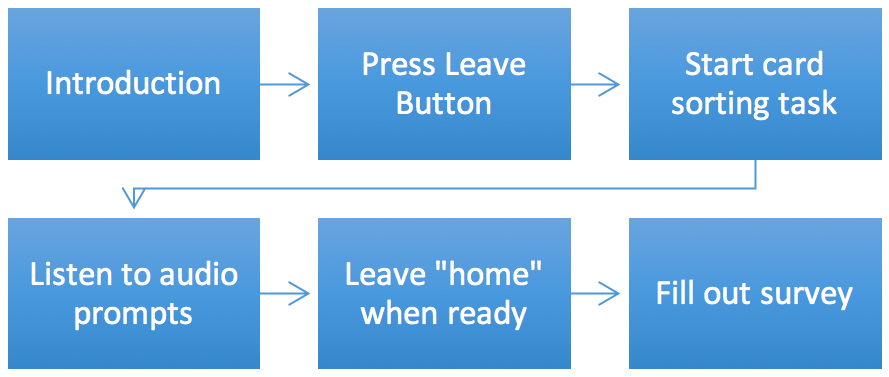
\includegraphics[width=5in]{Figures/Prototypes/CEP/CEPprocedure.png}
	\caption{CEP user testing procedure}
		\label{fig:CEPprocedure}
\end{figure}

The insights we got from user testing are: 1. Rated usefulness of information was mixed, but almost everyone found it helpful to preheat car or adjust temperature before leaving home. Information should be customizable – not everything needs to be said every day. But there is potential value in this information; 2. Exact action suggestion would be more useful than telling information about temperature or car status, for example, Some people did bring umbrella as suggested; 3. The most frequent thing to do before leaving home is to check keys \&{} the most frequent thing to do after arriving home is to turn on the light and take off shoes. So we could look at what people do when they sit in car.

\begin{figure}
\centering
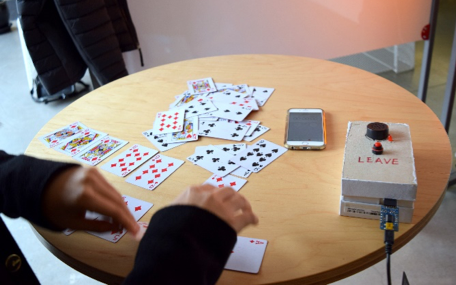
\includegraphics[width=5in]{Figures/Prototypes/CEP/CEPtest1.png}
	\caption{CEP user testing}
		\label{fig:CEPtest1}
\end{figure}

\begin{figure}
\centering
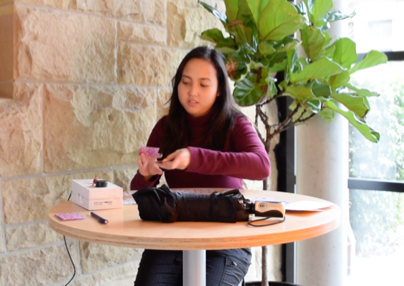
\includegraphics[width=5in]{Figures/Prototypes/CEP/CEPtest2.png}
	\caption{CEP user testing}
		\label{fig:CEPtest2}
\end{figure}

Other insights in terms of improving for future work are:

\begin{itemize}
    \item We could do a better job of setting up the scenario – some people were confused. 
    \item One person wanted a more interactive experience – the system would respond to their voice (could be done with Amazon Echo).
    \item Difficulty: we need to simulate a series of experiences in a whole environment rather than a single one. 
    \item Limitations of map: People were confused about the map’s route to their car. The route should rotate to match the exit’s direction; some descriptive information would also be helpful. If the map was pushed to phone, this would be more useful.
    \item Incorporate security element (e.g. car alerts authorities if you don’t show up after a certain amount of time)
\end{itemize}


\section{Dark Horse Prototype: car as extended room}

For our dark horse prototype, we were encouraged to try something crazy: Instead of bringing the car into the home, could we bring the home into the car? In other words, could we use the car as an extended room of our home? We believed that by inverting our problem, we might gain some valuable insights.

When autonomous driving becomes possible in the near future, using car as a movable room will become feasible, but that introduces problems with motion sickness. For now, we look at a parked car – a sound-insulated room with ample technology and comfort. We have discussed a lot of possible use cases: movie theater, meditation room, karaoke room, video game room, working space, bedroom, playground for kids, traveling showroom.

One of the advantages of using car as an extended room is to provide some kind of privacy. Our targeted users are younger generations who are much more likely than before to live with roommates or families until later in life, but still want freedom and privacy. Having a car as a place to relax and get away from routine lives could be a relief. And compared to a traditional room at your home, the car as a room will generate less noise to your roommates or neighbors but will be more private but will use high quality audio system in car.

We have tried two prototypes under the theme of using car as extended room. One is a in-car movie theater, the other is in-car sunshine meditation room. Provide a private movie experience in car, people can have freedom and privacy in watching any movie. For people that have a roommate/relatives, he or she can watch movie without any disturbance or interruption from others. Sunshine is missed in regions with long, dark winters, which can lead to seasonal affective disorder (SAD). Light therapy is a proven treatment for this condition. We made the car feel very cozy and relaxing, thus providing a personal sanctuary.

For the in-car movie theater, we used a white foam board as a screen with a projector in the trunk, a movie trailer for Interstellar was projected with the sound piped through the car speakers. Curtains covered the window to block light and add privacy. To enhance the movie experience, we could also add D-box (vibration and motion). 

\begin{figure}
\centering
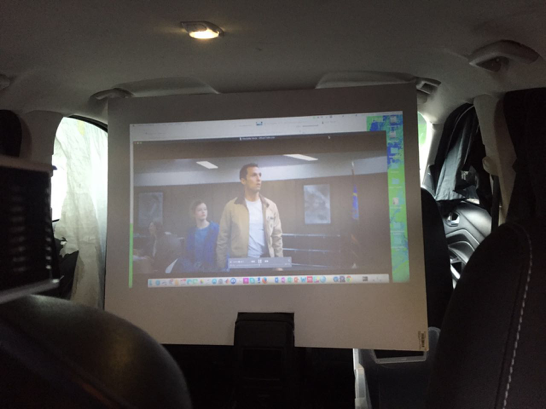
\includegraphics[width=5in]{Figures/Prototypes/DarkHorse/DarkHorseTheater1.png}
	\caption{In-car movie theater}
		\label{fig:DarkHorseTheater1}
\end{figure}

\begin{figure}
\centering
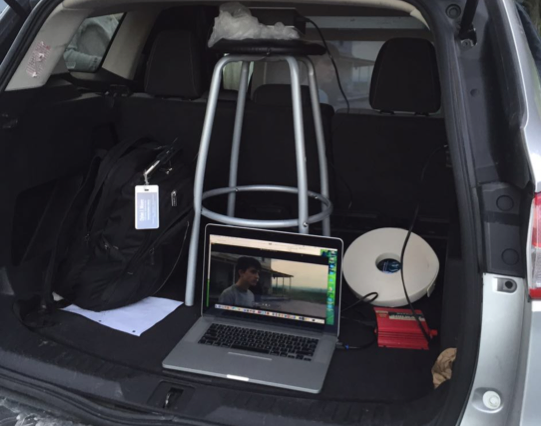
\includegraphics[width=5in]{Figures/Prototypes/DarkHorse/DarkHorseTheater2.png}
	\caption{In-car movie theater}
		\label{fig:DarkHorseTheater2}
\end{figure}

For the in-car meditation, we placed a diffused light shined beside the passenger, a sun-like warm light was also used. We also played New Age meditation music through car speakers.

\begin{figure}
\centering
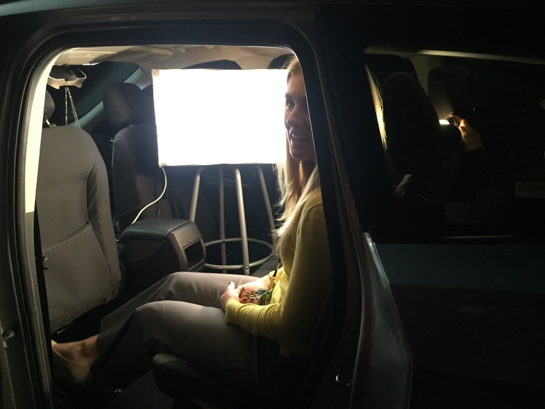
\includegraphics[width=5in]{Figures/Prototypes/DarkHorse/DarkHorseMeditation1.png}
	\caption{In-car meditation}
		\label{fig:DarkHorseMeditation1}
\end{figure}

\begin{figure}
\centering
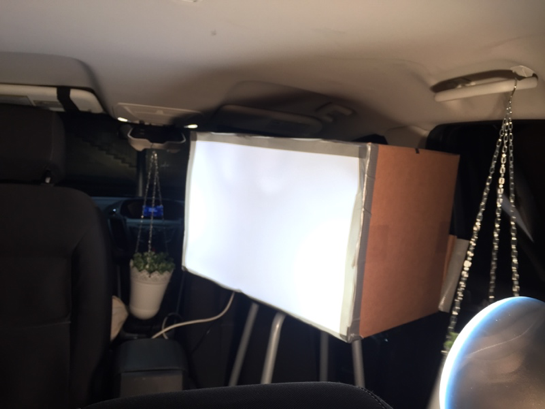
\includegraphics[width=5in]{Figures/Prototypes/DarkHorse/DarkHorseMeditation2.png}
	\caption{In-car meditation}
		\label{fig:DarkHorseMeditation2}
\end{figure}

We set up both prototypes in an SUV and tested them with some users. The insights we gained from interviews are:

\begin{itemize}
    \item Functional fixedness: Lots of people expected to watch the movie while driving, and were surprised when we said that it was for while the car was parked: people don't think of their car as an extended space while stationary - only think of it as moving from A to B. One driver mentioned that his car is associated with too much stress – commuting, work, etc. so he would not be able to relax in it.
    \item People were very comfortable and overall responded well to the experiences saying they were both fun and relaxing, but didn’t desire for them to be in their car. Some might pay a little extra while others would just want it in their home. Several expressed concern with setup time/hassle. 
    \item Several people said that they would like it if they had kids - the kids could watch a movie in the car while the parents had some peace and quiet in the home. Though the parents/families we talked to did not express much interest.
    \item One woman would go on a date in the movie theater as she liked the privacy.
    \item Power limitation - battery only lasted for 20-30 minutes of projection before it went low. We left the engine running for the meditation room. 
    \item Father with kids said he'd prefer it if he had an autonomous car and he could do it to/from work – his kids were with him and couldn’t sit still. Older man agreed he thought it would be useful for light therapy for people with SAD.

\end{itemize}

So going forward, there are three main takeaways: 1. The user test reiterates the need for simplicity in our final design – it can’t add any complexity to users’ lives; 2. There is a preconceived notion of the car as only transportation, which presents a potential opportunity if there was a compelling use case to develop it as a room when stationary. Cars are sophisticated machines that sit idle for much of their lives; 3. Cars are also a source of stress – how might we counteract the tendency for people to see cars as stressful experiences?


\subsection{FUNKtional System Prototype: Audi Scene}

For our FUNKtional System prototype, we want to solve two problems: (1) Smart home tech needs seamless integrated interfaces (set it and forget it) to manage technology and (2) Audi cars need to know users’ intention for departure to startup system (like an automated remote start). 

 Existing smart technologies are working on those problems: Amazon Echo is using voice control of home that connects to many devices; NuBryte home management system (out later 2016) sets lighting scenes for home, displays weather information, calendar, from a single source; Nimbus digital dashboard by Quirky displays simple information like “current time to home” and “tomorrow’s temperature”. The drawbacks with those devices are: More technological sophistication, but also more complexity. No dedicated physical interfaces. What if light switches changed their form depending on the day? It would get confusing.

Based on user needs, we image our solutions to be able to solve the problems in the approaches as shown in the following table.

\begin{center}
\tablefirsthead{%
\hline
\textbf{ } & \textbf{User needs to...} & \textbf{How might we address this need?} \\
\hline}
\tabletail{%
\hline
\multicolumn{3}{|l|}{\textit{\small{continued on next page}}}\\
\hline}
\tablelasttail{\hline}
\bottomcaption{From user need to approach}
\begin{supertabular}{| p{4mm} | p{60mm} | p{70mm} | }
		\hline 1 & Know his parents are safe. & He would feel better if his parents adopted smart home technology, but know it’s complicated. \\
		\hline 2 & Convince his parents to adopt smart home technology. & If he uses it and it’s simple to set up, then he can demonstrate to his parents and they will be more likely to use it.  \\ 
		\hline 3 & Control lighting, security, and temperature when he gets home to increase productivity. Wants control himself - doesn’t necessarily want home/car to “anticipate needs.”  & Placement of key fob triggers scenes in home, eliminating need to turn on/off lights, lock door, set music, etc.  \\ 
		\hline  4 & Boot Audi infotainment system before he gets to car to establish connection to internet. & Removal of key fob sends indication to car to begin 1 minute process. Could also set climate control. \\ 
        \hline 5 & Turn off lights, adjust heat, and make sure door is locked before he leaves home & Removal of key fob triggers “leaving home scene” that make sure no energy is being wasted and home is secure before he leaves. \\
        \hline 6 & Manage different media sources in his home. & Transfer media from car, start media when user arrives home if preprogrammed under scene. \\
\end{supertabular}
\end{center}

We designed a key fob storage unit that sets initial state of smart home when key fob is dropped into bin and signals car and home that user is leaving as key fob is picked up. As you walk in your front door, you can put your key fob into one of four bins that triggers a different “scene” for your home. E.g. relaxation mode turns on softer lights and nice music and work mode turns on brighter lights; It also continues media from car to home (e.g. sports match on radio to TV). It is customizable, and will eventually give smart suggestions. When leaving home, removal of key fob sends signal to car that starts up infotainment system (current time is appx. 1 minute) to connect to internet (e.g. pull addresses/traffic from Google Maps), and sets climate control. It also tells smart door lock to lock behind you (better than walking away and assuming door will lock behind you). 

\begin{figure}
\centering
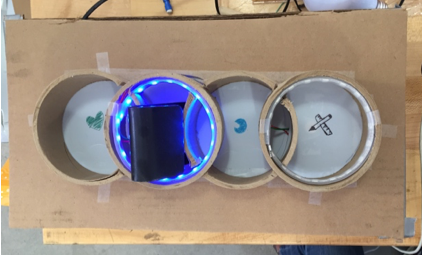
\includegraphics[width=5in]{Figures/Prototypes/Funky/FunkyPrototype.png}
	\caption{Drop the key fob to set different scenes for your home.}
		\label{fig:FunkyPrototype}
\end{figure}

\begin{figure}
\centering
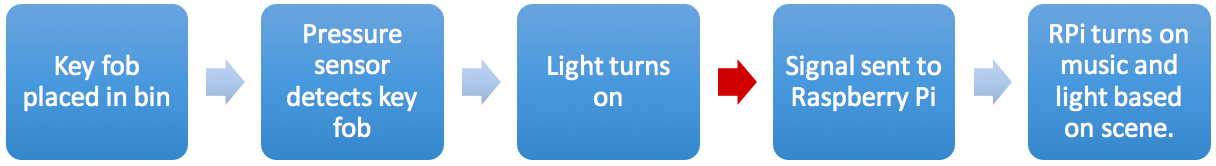
\includegraphics[width=5in]{Figures/Prototypes/Funky/FunkyPrototypePrinciple.png}
	\caption{Description of system working principle}
		\label{fig:FunkyPrototypePrinciple}
\end{figure}

From building this prototype, we have learned (1) online webserver and scripting is very powerful - we can leave many control function running on web server instead of portable hardware; (2) Lutron smart switch used different communication protocol and is not disclosed to customers, it is difficult to match them even for developers. But we were able to buy more generic ones; (3) However the simple physical operation is easy to use and could probably be adopted by even the most technologically compromised users.

And for future development, we have discussed the following potential features:

\begin{itemize}
\item Light string can display state of home through colors as user approaches to retrieve fob.
    \subitem Red: something needs to be addressed (e.g. door or window open)
    \subitem Yellow: almost ready to go, and system can take care of it (e.g. light on)
    \subitem Green: all set to walk out the door (all lights off, etc.)
\item RFID tags for important items detected by system - intelligent state selection (e.g. if briefcase is detected, then car will know user is heading to work). Also could alert user if something is forgotten at home or if something is left in car.
\item Address security desire in smart home –incorporate a monitoring element (e.g. if a package is delivered, door can open and system can record delivery to make sure nothing is stolen).
\item Wireless charging of key fob while it is in the device.
\end{itemize}
\section{AudiDefender}
\subsection{Description}
% Shouldn't we leave the distinction between HPI and Stanford out?
"Audi Defender" is the most complete prototype that reflects our vision with regards to security. According to design requirements, the system should securely detect the keyfob and verify its identity, and then enabling quick arming and disarming of home security system. The system should also interact with users and provide instant feedback about car and home, presumably but not limited to a visual display. Along with Stanford's Funky prototype, we designed a bin that would be placed in people's home to represent Audi's brand. The system wirelessly connected to a touchscreen that displays security status of home and car as well as car's driving range. These information are deemed crucial in the transition space of car and home. 

We think the security angle is appropriate for Audi to tackle with in this joint realm of home and car. Firstly, people have trust in car's security system, and Audi have sophisticated related technology that can be relatively easily used in this system. Secondly, leveraging existing car security system could make interface simple and reduce the need for another isolated security token. Finally, it is the security related information that people mostly want to know about their car while they stays at home. And the (visual) interface of such a device can well serve that purpose.

In summary, our system is a physical presence of the car in your home. Presumably, it is placed on the table and looks cool like other Audi accessories [\url http://audicollectionusa.com/Accessories]. It works with user's keyfob to smooth the secure transition from home to car and provide valuable security status to user to let them feel carefree about their home and car. A video of how we imagine this system improving users' lives can be found here \url{https://youtu.be/NIcLD-aaaGM}.

\subsection{Implementation}
\begin{figure}[ht]
\label{Fig.AudiDefender}
\centering
	\includegraphics[keepaspectratio, width=5in]{Figures/Specifications/AudiDefender.JPG}
	\caption{Stanford's Prototype, a electronics device to put on a table inside the home. Its touchscreen shows car and home related critical information, and it interacts with a special Audi keyfob to arm and disarm smart home security system. At the top of it there is a bin to store and verify user's Audi keyfob}
\end{figure}

As depicted in Fig. \ref{Fig.AudiDefender}, this prototype is designed to be placed on a table in the home, possibly near the front door. It is primarily made of black foam board. At the front side, there is a touchscreen to provide visual interactive interface to the user. It also plays alert sounds in emergency. At the top of the device there is a bin to place the keyfob, and user need to interact with our system using our special Audi keyfob. Electronics is placed inside the box and a large battery bank support the mobile use of electronics. The touchscreen shows security status of the home and car, whose state transition is illustrated in Fig. \ref{Fig.StateChange}

\begin{figure}[ht]
\label{Fig.StateChange}
\centering
	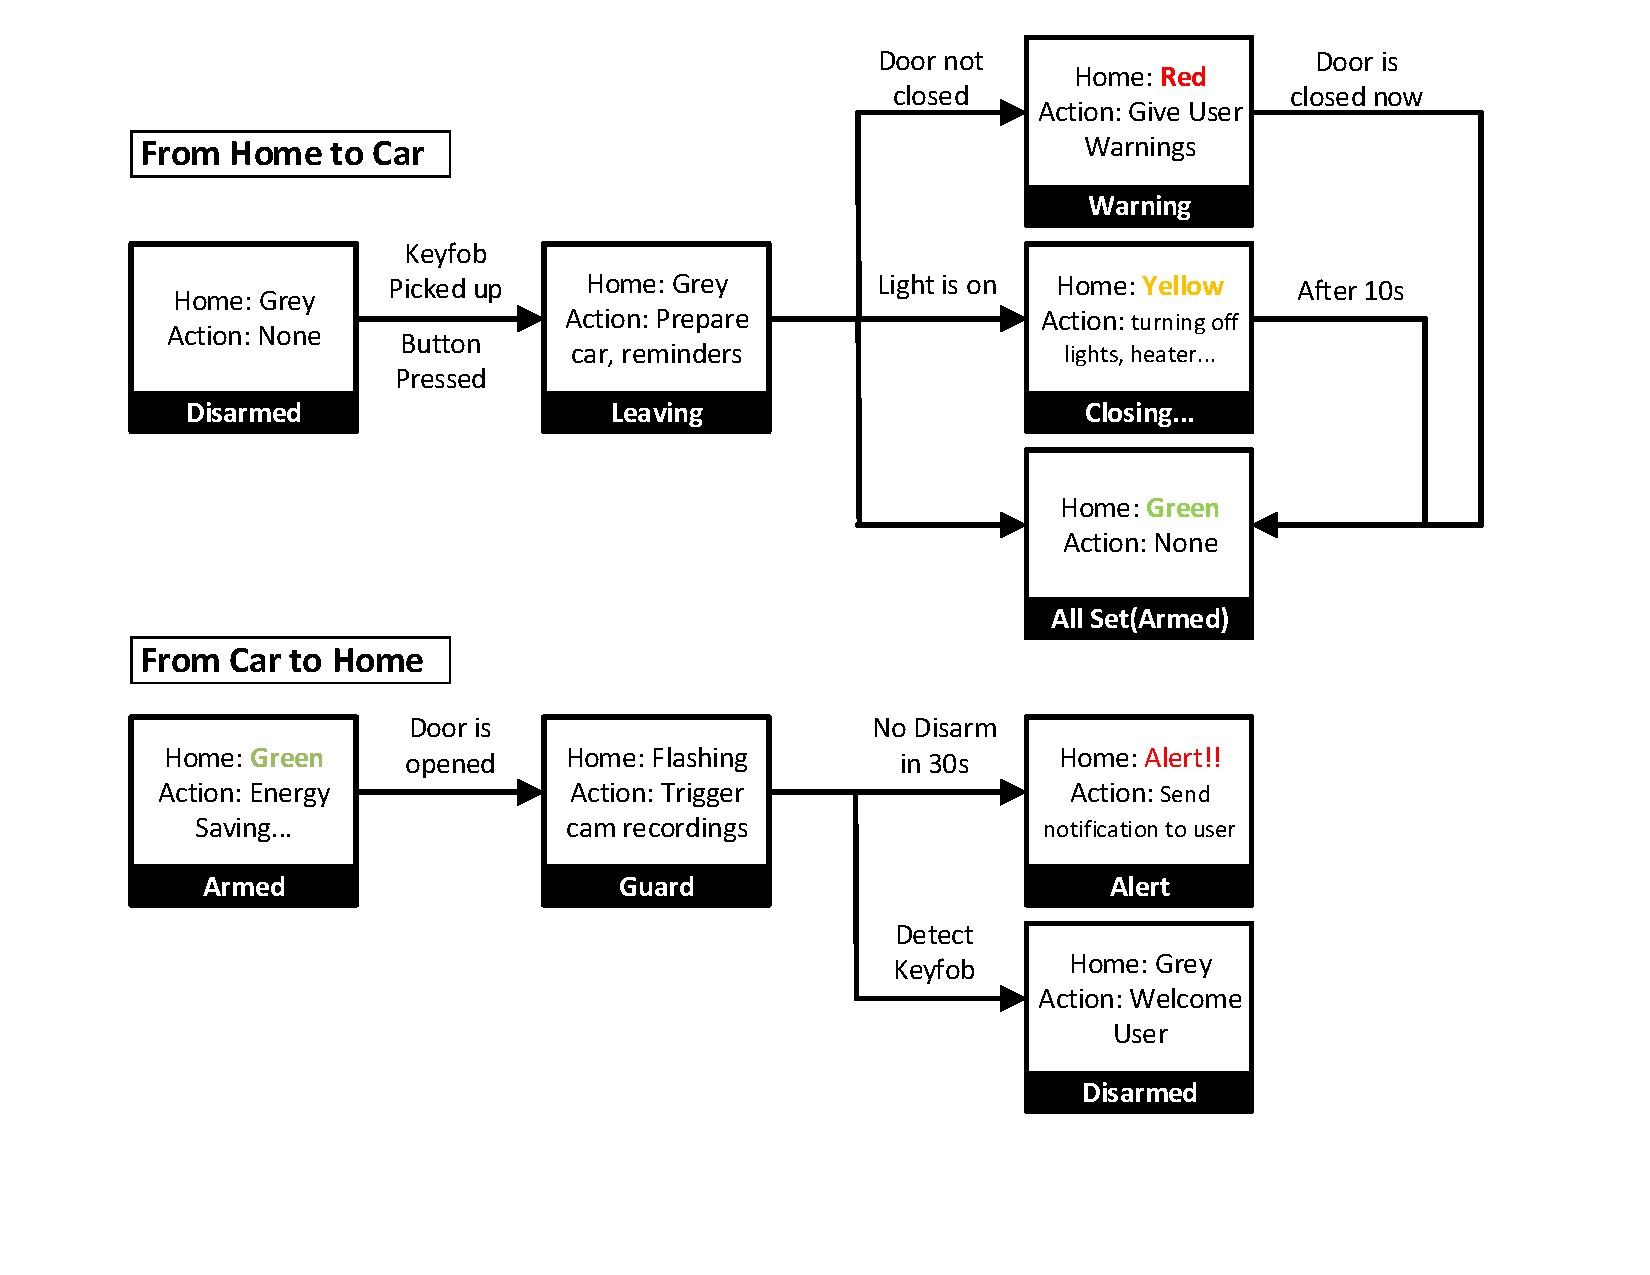
\includegraphics[keepaspectratio, width=5in]{Figures/Specifications/StateDiagram.pdf}
	\caption{State transition diagram for both case for going into home and leaving home. It described which color to display for the home icon in that touchscreen. In a certain state, there are smart home activities and settings associated with the status.}
\end{figure}

The bin provides a place to store the keyfob, and we check the keyfob using RFID(Radio Frequency Identification) chips and reader. RFID is a short range communication method, so it avoids the hackability of long-range radio signals. However, we used only a "passive" card in the keyfob, which code can be read by any other RFID reader. Going forward, we definitely need to use a more sophisticated secure communication method and advanced techniques like rolling codes. Accordingly, we should consider factors like the battery life of the keyfob, and sophisticated protocol. Henceforth in our prototype, in order to avoid complexity in prototyping, only simple RFID communication is used. A 125kHz RFID card is placed into the shell of a Audi keyfob to create our special keyfob, and a card reader kit is placed inside the bin. When the special keyfob is moved towards the reader, the reader gives off a beep sound and send the unique identification code of card via serial port. By matching the signal with recorded code in system, the controller unlocks the security system.

We used Raspberry Pi 2(RPi) as our central controller. It runs a LINUX based operation system, and can thus achieve versatile functions. RPi has more memory resources and available open library than microcontrollers like Arduino, but it has drawbacks in handling real-time tasks. We used python for most of the programming and vncserver and SSH to communicate with the RPi in Wifi netword during programming and debugging.

\begin{figure}[ht]
\label{Fig.AndroidInterface}
\centering
	\includegraphics[keepaspectratio, width=5in]{Figures/Specifications/AndriodApp.png}
	\caption{Enlarged touch screen, enabled by a Android App. It has simple intuitive state indication, and after user pressed the icon, detailed information would be prompted}
\end{figure}

The touchscreen display in our prototype is a Huawei smartphone running android system. The android interface is designed as showed in Fig.\ref{Fig.AndroidInterface} The icon of car and home associated with different colors shows the security status as fully explained in Fig. \ref{Fig.Icons} . After the user long pressed the icon, detailed text notification will be prompted. In our prototype, we lacks input from car, so we made the car icon color changing for long-press to facilitate demo.

\begin{figure}[ht]
\label{Fig.Icons}
\centering
	\includegraphics[keepaspectratio, width=5in]{Figures/Specifications/Icons.jpg}
	\caption{Different icons and explanation for the interactive touchscreen. Notice that we only implemented the automatic change of home's icon in the prototype. We still lack car side's input.}
\end{figure}

For simplicity, we used Bluetooth to communicate between RPi and smartphone. A serial port is established via Bluetooth, and the Rpi send code in the format of "H[State]\#[Information]" ([State] is a number from 1 to 4, and [Information] is a string)to control the displayed home status. Since in our system we cannot automatically detect the leave of keyfob, we need a switch to tell the system the change of state. We implemented via the smartphone, when the home system is disarmed and user pressed the home icon, a message of "LEAVING\#"is sent to RPi and it will change system status accordingly.

There are many tasks for the systems to handle during the Leaving state. Actually it is a requirement for the system to reliably detect user's intention of going to the car. If the ecosystem obtained that intention to car in advance, it can boot the infotainment system to avoid long reboot time and preheat the car. The ecosystem can also present mobility related information and reminder to prepare the trip like we did in our CEP. However, in our prototype, we temporarily saved these aspects for future development and focus on the smart home aspect as expalined in \ref{Fig.StateChange}. After the user dictate their intention to leave, the system check the status of home. If some major door or window is still open, the system display red home icon and require user to fix that. If some lights is still on, the system display yellow icon and it means some issues is automatically taken care of by the smart home and icon quickly changes into green meaning you are free to leave. By providing simple visual feedback, user will have overview and control of their home and they can always look into details.

Initially, the system is built upon scratches from related open-source RPi  projects. The most extensive one of them is "PrivateEyePi" [http://projects.privateeyepi.com/], which is the foundation of some early developments. For debugging, we built a system  that connects LEDs, buttons, LCD to Rpi. But we later abandoned those and transferred most of the interface to the touchscreen. We have also attached buzzer to RPi, but for final prototype, we used sounds of the smartphone instead to simplify the hardware. 

According to the system diagram, the system should connect to existing smart home to get necessary input about the status of the home. Due to the complexity of commercial system, especially the communication part, we must simplify this part to certain extent. Firstly, we have built a small scale home paper model that use contact switch (relay) to detect the status of the window and doors as showed in Fig. \ref{Fig.SmallHome}. This modelling resembles the actual home security sensor quite much, but we found this model is difficult for user testing and smart home system is an unnecessary complexity in our prototype.

\begin{figure}[ht]
\label{Fig.SmallHome}
\centering
	\includegraphics[keepaspectratio, width=5in]{Figures/Specifications/SmallHome.jpg}
	\caption{A small scale home model build from cardboard. Blue rectangle illustrates the contact sensor that indicate the on/off status of windows and doors. }
\end{figure}

\begin{figure}[ht]
\label{Fig.VirtualInput}
\centering
	\includegraphics[keepaspectratio, width=5in]{Figures/Specifications/VirtualInput.png}
	\caption{A virtual version of the smart home architecture. By pressing the button on the webpage, we give system input about home status, thus eliminating the need to implementing smart home hardware in our prototype. In our vision, we assume this Audi prototype will not change the basic smart home architecture, but to communicate with its controller}
\end{figure}

Later, we adopted a simulation method to get virtual smart home input from a webpage. The picture Fig. \ref{Fig.VirtualInput} shows that we can directly dictate status of window, door and lights. It also has buttons to directly change the state to facilitate debugging. In order to create webpage, we firstly used a python module called "WebPy" and later transformed to "Flask" combined with simple HTML. These newly developed tool is quick to use, but due to our inexperience in front-end programming and Linux, we only implemented basic interfaces and logic. The use of webpage also arise the use of multiprocessing, since RPi needs to process webpage response, communication, state transition based on home input simultaneously. Basic python multiprocessing module is used and need further explored to address some unreliability in existing system.

We have performed several technical tests throughout the development and we can see that communication protocol and growing complexity is a challenge. We improved the structure of the device to make it fit for electronics and battery, better looking, screen tilted for easy touch and display. We primarily tested at the entrance of Stanford bookstore. And at the parent's day, it appeared lots of parents have Audi cars and many of them has experience with security system, which makes them good representatives of our persona. They generally respond excited to our prototype. The physical presence of the car in home itself seems innovative to them too.  Many users told that this device would reinforce the habit to put keyfob in a certain place, and many of them likes to do so to restrain from forgetting the keychains. …

\section{AudiSeamless}

AudiSeamless is a system that wants to make forgetting things a thing of the past, at least with respect to what a user needs to take care of before leaving the house. It contains all of the findings of previous prototypes\footnote{described in the appendix under \ref{sec:HPIPrototypes}} but goes more in the vain of providing a system that is of use at home, as opposed to the earlier prototypes which were more useful on the road.

During interviews, we found out that there are three areas that people need to be assured about before being able to leave their homes with an easy mind:

\begin{enumerate}
    \item House: This includes making sure the heating is turned off, that all windows are closed and that the home security system is armed.
    \item Packing: Users have to be sure that they packed everything they will need like luggage before a longer journey or their sports items for their training.
    \item Car: This includes knowing where the car is parked (a challenge in big cities, especially when sharing the car with family members), whether the car's windows are frozen and how much gas is left in the tank.
\end{enumerate}

\noindent{}AudiSeamless collects information for every connected device in these three areas and makes this information available to output devices like smart phones, voice assistants like Amazon Echo or our corresponding idea, \textbf{AudiBits} (see Figure \ref{fig:AudiSeamless}). The intended use case for AudiSeamless is to provide the necessary information at the right time and place for users so they forget things less often. So when a user is about to leave their house, AudiSeamless is supposed to indicate to her that she forgot to pack her sports bag for the night.

AudiBits (see Figure \ref{fig:AudiBits}) are specifically tailored to this use case: They are small, single-purpose displays that show information about one specific item. They can be placed in any part of a user's home to maximize usefulness to them. So if the user had connected her AudiBit with her sports bag and placed it near her house door, she would recognize that she had forgotten it before leaving the house, thus saving her time.

\begin{figure}[ht]
\centering
	\includegraphics[keepaspectratio, width=\textwidth]{Figures/Specifications/AudiSeamless}
	\caption{The AudiSeamless concept works with home and car data sources and distributes the collected data to different output devices like smart phones.}
	\label{fig:AudiSeamless}
\end{figure}

\begin{figure}[ht]
\centering
	\includegraphics[keepaspectratio, width=\textwidth]{Figures/Specifications/AudiBits}
	\caption{Two AudiBits. The one on the left shows an item that has been taken care of and the one on the right shows the gas tank, both with an icon and with a color (green = tank is (almost) full, yellow = tank is about halfway filled, red = tank is (almost) empty)}
	\label{fig:AudiBits}
\end{figure}

The AudiBits purposely represent a semi-automatic approach to keeping an eye on the users homes and cars. Many use cases of AudiSeamless seem like they could also be completely automated. Instead of reminding the user or displaying information to him the system could act itself without interacting with the user, one could think. Instead, we have identified that our users want to have the feeling of being in control, to have the last word. The AudiBits build on these findings by displaying bits of information to the user and letting her interact with them when she wants to. They stay unobtrusively in the background if she decides to ignore them.

We tested this idea with potential users and received positive feedback to the idea itself and the underlying need but also heard from many people that they don't see the need for small displays like the AudiBits since their smart phones can also display the same data. We agree that this is possible but still find that AudiBits offer a significant improvement: They are always visible at places where users will see them when necessary as opposed to a smart phone with which users have to first open up an app or take them out to look at a notification and which are not always with the user.

We also found out that merely displaying the status of a forgotten thing is not enough for users because they want to be able to act upon it. For example, if the display shows that the user's car windows are frozen, he wants to be able to turn on the heating so that he can start driving as soon as he reaches the car without having to get rid of the ice on the car windows first.

Another finding is that people think of things they need to do when they're home while they're out. AudiSeamless and especially AudiBits could be a good way of resolving this: While out, the user could send whatever they want to remember to AudiSeamless which an AudiBit set up for this purpose could then display so the user sees it when they get back home.

\clearpage


\section{User Journey}
Our persona Linda has to get up very early in the morning, and really is not a morning person, so she's often still groggy when she leaves. As a result, she forgets to bring sports equipment for days when she exercises, or an umbrella when it's going to rain that day. AudiSeamless will remind Linda that Tuesdays and Thursdays are her CrossFit days and that she should bring her gym bag if she does not already have it. As a result, less of her classes will be skipped due to not having the right equipment.

When Linda gets home from a busy day at work, and then CrossFit, and nobody else is home, the last thing she wants to do is worry about forgetting to disarm her security system, have the alarm go off, and have to pay a fine for a false alarm. However, she does like the peace of mind that her home is being looked after during the day, as there have been a couple of break-ins in her neighborhood recently. She also likes to know that the home will be secure when her kids get home from school, and that they can each disarm the system with a mini Audi key fob on their keychains. Her daughters love showing off the key fobs at school.

Using AudiSeamless, she gets peace of mind of the home security system while not changing her daily routine at all. She often keeps her keys in her purse, so when she walks in the door, the key fob's presence is automatically detected and the home security system  automatically deactivates. She might even want to set up a light or two to go on at that time, so that she can easily find her way through her front hallway. 

However her family members like to store their keys, either in a bag or in their pockets, the system can detect their presence and store their keychains if desired (see Figure \ref{fig:Vision}). The system also interacts with modular displays that show basic information about her home and car. She can make sure her car is okay when she's inside her home.

\begin{figure}[ht]
\centering
	\includegraphics[keepaspectratio, width=6in]{Figures/Specifications/vision.jpg}
	\caption[Design vision overview]{An elegant bowl that wirelessly detects the presence of the Audi key fob to automatically disarm a home security system when the user arrives home. The bowl works in tandem with a set of modular displays that show important information about the state of the home and car and placed anywhere the user desires. Upon departure, the user’s indication of departure prepares their Audi for the journey ahead by setting car’s climate, heating electric batteries, connecting car to internet, and reminding them of their parked car location.}
	\label{fig:Vision}
	
\end{figure}

\section{Ongoing Development}

There are some remaining questions we are currently investigating.

\begin{itemize}
    \item How should the system interact with multiple key fobs in use with access to the home security system and car?
    \item What is the ideal placement for the display or whatever visual feedback users receive about the state of their car and home? Should it be integrated with the system or modular to be able to be placed anywhere?
    \item What is the best way to communicate home and car-related information? We will test interfaces including, but not limited to, lights, audio, visuals, all through a display, smart phone, and/or the key fob itself.
\end{itemize}
    
\noindent There are also many technical improvements to be done. We need a seamless integration of the physical device and electronics and we will let the user interact with our prototype rather than showing its function by ourselves. The main challenge would be communication, reliable state change, and interaction design. However, due to the tight security of the Audi key fob system and multimedia interface, for obvious reasons, we will have to simulate the key fob communication and car communication using other protocols, so we can spend more of our effort on fine-tuning the experience we want to give our users.  

%%%%%%%%%%%%%%%%%%%%%%%%%%%%%%%%
\chapterimage{ChapterImages/Planning2}
\chapter{Planning}
\label{project-planning}

% %%%%%%%%%%%%%%%%%%%
% \begin{remark}\color{blue}
% Teams with global partners face special challenges in  terms of organization, project management and planning.
% It is a truism that organizational burden goes as the square of team size. 

% To address these issues, we ask each local+global team to prepare a \textbf{plan for Winter quarter} to include in this section. You have just accomplished a first, rough critical function prototype (CFP or CEP) and you have given a presentation and written a document that captures the current state of your vision and findings. You have learned who can do what and how much work it really takes. You are motivated to make Winter go more smoothly and to ``take control'' of your project instead of living from week to week.
% \normalcolor \end{remark}
% %%%%%%%%%%%%%%%%%%%

\vspace{1em}

In the following chapter we will evaluate what we did in the winter quarter, how we did it, which tools we used and which resources we allocated. Furthermore it contains an outlook into the spring quarter, our next steps and our personal reflections on the ME310-course at this point.

\section{Project Progress}

\subsection{Review of Winter Quarter}

During the fall quarter, we have explored different spaces between home and car, and successfully built a critical functional prototype (automatic car washing robot in the garage) as well as a critical experience prototype (a voice assistant inside the car to manage the home). At the end of the fall quarter, we arrived at a consensus that by talking about uniting home and car, we are focusing on smoothing the transition between those two places.

Therefore, during the winter quarter, both Stanford and HPI team built prototypes aiming to improve the not yet smooth experience when transiting between home and car. The Stanford team mainly focused on interaction within the home while HPI mainly focused on car related interaction before we eventually converged to car-home-transition related interaction for our last prototypes (also cf. figure \ref{fig:prototype_overview}). 

The Stanford team started with a critical function prototype, focusing on the leaving home experience. We designed a leave-home button that will prompt the user information about navigation, weather, things to bring and so on, preparing the coming trip for the user. The main takeaway was people might not want to have a nagging mom when leaving home and showing all the information through voice was not plausible. Then, in the dark horse prototype, instead of bringing the car to the home, we bring the home to the car, using the car as an extended room of the home. We built a movie theater and a sunshine meditation room in an SUV and it was actually much more plausible than we had thought before. For both the funky and functional system prototype, we built a physical device that sits inside home, showing information and sending a command upon leaving or arriving home. We designed a key fob storage unit that the user could set the scene of his home with by dropping the key fob into a certain beam that represented a lighting and audio scene. Then we realized that there was not a compelling enough use case that users would buy the device for. For the functional prototype, we decided to focus on security. We built a key fob storage case and with a screen that shows home and car status represented by different colors. Furthermore, it reduced false alarms because you could disarm your security system by dropping the key fob when you arrive home instead of entering a complex code.

The HPI team prototyped an in-car voice assistant during the fall quarter with which the smart home could be configured and controlled while in the car and driving, thus making use of otherwise wasted time in the car. The general feedback to it was positive, however for our dark horse prototype we went into a completely different direction to explore other possible orientations for the project. As suggested by the dark horse prototype, we went crazy and assumed teleportation is possible. We designed a shelf that can be placed anywhere inside the house and its compartments correspond to different compartments of the car such as the trunk or glove box. Whatever is placed in a compartment - whether it is in the shelf or the car - is automatically teleported to the corresponding other compartment as well, thus making carrying things from the car to the house unnecessary and enabling the user to pack things into the car without leaving the house. We found out that users especially liked that they do not have to carry their errands inside after doing the grocery shopping, and that they think they would forget less things if they had such a shelf serving as a kind of reminder since it is placed inside their apartment and they would have an overview over everything that is packed already. Based on the pain of having to carry groceries, we designed a self-driving cart that integrates seamlessly into the car as our funky prototype. We found out that people generally liked the idea of it, however we decided to go back to the reminder-need for our functional system prototype to better meet the constraints of our problem and the challenge as well as to converge with the Stanford team. As a result we came up with the AudiBits that can be placed anywhere inside the home and help the user to remember to pack things and to remember and check information about their car and home status.  

\begin{figure}
\centering
\includegraphics[width=5in]{Figures/Planning/Prototype_Overview}
	\caption{Overview over the prototypes created by Stanford and HPI during the fall and winter quarter.}
		\label{fig:prototype_overview}
\end{figure}

The Stanford team will visit the HPI from March 20th to March 27th. We are going to plan for the spring quarter and converge for the final design.

\subsection{Plan for Spring Quarter}
% Layout a plan for spring. Make sure your team reaches consensus on this. It is a critical element of how your liaisons (and the TTeam) will evaluate the status of your project. We will revisit this plan in spring SGMs.

%    What will your team do next? When \& how will milestones be accomplished, and by whom?
%    How will the budget be spent?
%    Any lessons learned from your time management this quarter?
%    How will you meet the final deadline of EXPE? 
The global team of students from HPI and Stanford will have its next in-person meeting the week after handing in this documentation. We will use this opportunity to fully converge our different approaches to the transition between home and car, in terms of visual design, the needs on which we base our design and the problem which we both are trying to solve. During this time we will also agree on which parts of the system which part of the team will implement (that is, if it is possible to split the system): With regards to the past prototypes and the background of the team members we can already determine that Stanford students have a penchant for good design and that HPI students are more focused on basing their implementations on needs discovered with their users so it would make sense to distribute tasks accordingly.

During the Spring Quarter we will keep our two weekly meetings to synchronize our activities as closely as possible given the time difference of 9 hours between HPI and Stanford students.

HPI students and Stanford students will meet again in Stanford at May 22nd to prepare for the final deadline. HPI students are willing to work full-time for the project to reach the final deadline.

\section{Team Management}
Each team decided to assign one team member to a certain area of responsibility (called "officer") to keep a better overview and split the workload. For HPI these were a space officer (Jonathan), a communication officer (Jonas), a financial officer (Johanna) and a documentation officer (Martin). Stanford had assigned roles of communication officer (Dylan), documentation officer (Maggie), and financial officer (Zhipeng) continuing from the fall quarter. Apart from introducing these roles on HPI side, we  did not make significant changes to our team management. 

\subsection{Communication and Collaboration}
We kept our timeslot of Friday, 10:00 AM PST and 7:00 PM CEST, for our weekly video conference. In addition to that, we held a second regular weekly meeting on Wednesday, 9:00 AM PST and 6:00 PM CEST, that we conducted in text chat form. This proved to be helpful, since it turned out to be a quite effective communication method with a built-in protocol.

We found that our agenda setting and strict moderation did not provide much added value last quarter. This could be due to the fact that we did not have good mechanisms in-place to review protocols of past meetings and follow up on action items. Our meetings in the winter quarter appeared to be less structured, but we did not notice a drop in the quality of our discussions.

\subsection{Used Tools}
For our video conferences we sticked to GoToMeeting. For the second weekly meeting in text form we used Slack. Regarding our documentation, we had discovered during the writing of our fall report that Overleaf had become very slow compiling our Latex files, so we re-evaluated our choice. We discovered that ShareLatex did the same job much quicker and are therefore using it now to collaboratively write this report.

We sticked to OneNote as our place to gather most of our documents and information. Over time, all team members started appreciating it as a valuable tool. During the winter quarter, we made it accessible for our liaisons for their reference. Complementing OneNote, we use OneDrive for the sharing of larger files - mainly photos and videos of testings and prototypes.
 
\section{Budget}
\label{sec:budget}

Both the HPI and the Stanford team are provided with a budget for buying necessary materials to conduct user studies and to build prototypes. The Stanford team has a dedicated budget for each quarter and unused budget rolls over to the next quarter. The HPI team has an overall budget for all three quarters.

\subsection{HPI Budget}

The HPI team has an overall budget of \euro5,500. At the current point the team has spent \euro320.88 for building prototypes and rewarding testers. A detailed list of the expenses of the current and the last quarter can be found in table \ref{tab:budget_hpi}. The HPI team has only spent a very small fraction of its budget so far since no electronics and only very basic prototyping materials were needed. We expect to spend more money in the coming quarter when it comes to implementing and realizing technical solutions but we believe that we will not have any problems staying within the remaining budget. 

\begin{table}[!ht]
	\centering
		\begin{tabular}{| r | r | r |}
		%\begin{tabular}{| p{50mm} | p{17mm} | p{17mm} |}
		\hline
		\textbf{Purpose}	& \textbf{Date} & \textbf{Amount} \\
		\hline
		Chocolate for participants of user study & 11/23/2015 & \euro21.18\\ \hline
        \multicolumn{2}{|r}{\textbf{Spending Fall Quarter:}} & \textbf{\euro21.18} \\ \hline
        Chocolate for participants of user study & 01/23/2016 & \euro29.70 \\ \hline
        Equipment for Dark Horse testing (shelf and things to pack) & 01/27/2016 & \euro47.78 \\ \hline
        Preparation of Dark Horse testing car & 01/27/2016 & \euro35.89 \\ \hline
        Material for Funky Prototype (hand truck, tape, boxes) & 02/03/2016 & \euro94.67 \\ \hline
        Shopping vouchers for Funky-testers & 02/06/2016 & \euro75.00 \\ \hline
        Collaborative LaTeX license (ShareLaTeX) & 03/14/2016 & \euro16.66 \\ \hline
        \multicolumn{2}{|r}{\textbf{Spending Winter Quarter:}} & \textbf{\euro299.70} \\ \hline \hline
        \multicolumn{2}{|r}{\textbf{Spending Total:}} & \textbf{\euro320.88} \\ \hline
        \multicolumn{2}{|r}{\textbf{Remaining Budget:}} & \textbf{\euro5,179.12} \\ \hline
	\end{tabular}
	\caption{HPI Budget Overview }
	\label{tab:budget_hpi}
\end{table}
    
\subsection{Stanford Budget}

The Stanford team has an annual budget of \$8000, and overall we have spent only a small fraction of it during the fall and winter quarter. Most the spending is related to benchmarking hardware, prototyping electronics, German Visa, and the SUDS. Considering the anticipatory spending for fall and winter, we have plenty of them left for Spring quarter. 

Given that our prototype will focus on the physical interface of car and home, and due to simplicity issue, we will simulate most of the information flow and activities at the car side and home side. And for spring quarter, most of the spending would be related to prototyping electronics and manufacturing parts. Since we may explore other interfaces, such as gesture control and hologram, the cost associated with these novel hardware would be much higher. Overall, according to the speed of current spending, we believe we have enough budget for spring development, and it is highly possible that we have some budget left at the end of the year.   

\begin{table}[!ht]
	\centering
		\begin{tabular}{| r | r | r |}
		%\begin{tabular}{| p{50mm} | p{17mm} | p{17mm} |}
		\hline
		\textbf{Purpose}	& \textbf{Date} & \textbf{Amount} \\
		\hline
		Benchmarking smart home hardwar & 11/2/2015 & \$150.01 \\ \hline
		Benchmarking at Target Open House & 11/1/2015 & \$44.16 \\ \hline
		CFP, car body pieces  & 11/15/2015 & \$14.31 \\ \hline
		CFP, cloth, towel, cleaning solution etc.  & 11/14/2015 & \$46.83 \\ \hline
		Fall Team Mileage   & 12/1/2015 & \$64.41 \\ \hline
		Working meal with liasons  & 12/6/2015 & \$117.10 \\ \hline
        \multicolumn{2}{|r}{\textbf{Spending Fall Quarter:}} & \textbf{\$436.82} \\ \hline
        CEP, car rental & 1/19/2016 & \$62.48 \\ \hline	
        Darkhorse, lights for prototyping & 1/24/2016 & \$179.91 \\ \hline	
        Benchmarking gestural interface, and augmented reality & 1/31/2016 & \$141.69 \\ \hline
        Prototyping, 2 Raspberry Pi starter Kit & 2/2/2016 & \$139.98 \\ \hline	
        Electronics, RF transducers, speaker, pressure sensor, etc. & 2/3/2016 & \$78.07 \\ \hline	
        German Visa Related for Zhipeng and Maggie & 2/16/2016 & \$266.19 \\ \hline
        Prototyping, Wireless Outlets, Switch, LCD etc. & 2/6/2016 & \$76.10 \\ \hline	
        RFID modules, LEDS, sensors and accessories & 2/18/2016 & \$133.09 \\ \hline	
        Modeling Material & 2/21/2016 & \$39.09 \\ \hline
        PLX Bluetooth Module and Dongle & 2/5/2016 & \$72.30 \\ \hline
        Prototyping, Logic Analyzer & 2/11/2016 & \$126.85 \\ \hline
        Functional, Large Battery Bank & 2/23/2016 & \$40.90 \\ \hline
        SUDS & 2/10/2016 & \$476.20 \\ \hline
        Winter Team Mileage & 3/1/2016 & \$52.38 \\ \hline
        \multicolumn{2}{|r}{\textbf{Spending Winter Quarter:}} & \textbf{\$1,885.23} \\ \hline \hline
        \multicolumn{2}{|r}{\textbf{Spending Total:}} & \textbf{\$2,322.05} \\ \hline
        \multicolumn{2}{|r}{\textbf{Remaining Budget:}} & \textbf{\$5,677.95} \\ \hline
	\end{tabular}
	\caption{Stanford Budget Overview }
	\label{tab:budget_stanford}
\end{table}

\section{Reflections}
\subsection*{Martin Fritzsche}
I choose to take part in the ME310 course because of the prospect of gaining insights into a totally different approach on how to tackle a project and exercising this from the very beginning up to a pretty much presentable prototype. The design thinking process was completely new to me at the beginning of the course, which imposed quite some challenges. I sometimes felt a little lost and was very thankful to have my team partners which had some previous knowledge of the process and thus could guide and jump in by giving a more concise frame on what to do at which stage. Right now I have a pretty good idea of the process and feel like I am actively contributing.

That last three months passed by very quickly. While building and testing our different prototypes we explored more and more of the design space and found some interesting directions to follow. With the latest prototypes from Stanford and HPI imagined as two sides of the same system we finally have a unified vision down the road, something that I found hard to see before.

I like the structure of the course with the weekly presentations in a not-to-formal matter. They help by forcing us to rethink the week and put our findings in a nutshell. I am still amazed by our results week after week, since at the beginning of every week I mostly felt overwhelmed by all the possible directions to explore and tasks to fulfill. It felt hard to try to converge in one direction after having explored such a wide variety of ideas. 

Working together with our Stanford team partners has been working out very well. I very much look forward to the visit of our partner team next week. We planned an intensive week, discussions and planning on a unified vision and prototype to go for in our final three months 

I am confident that we can keep up our good spirit and build an intriguing and original prototype.
\subsection*{Jonathan Herdt}
\subsection*{Zhipeng Hu}
ME310 is a challenging and rewarding process. In this environment, I am able to adapt to some behavior pattern of design communities, which is refreshing and complementary to my engineering mind. More specifically, in this quarter, I improved communication skills and learned empathy in decision process. A major part about winter quarter is how to embrace uncertainty, it is definitely more challenging than it firstly sounds to me. It requires remarkable self-motivation for every team member. I appreciate very much the unique contribution of my team, we are always able to make things happen. 

A consensus among Stanford team is that we should do a better job at selling a vision and product. For some of the SGMs, we could make it better by articulating a story that emphasize one aspect of the problem or need. And the effect also depends on the way we present it, more enthusiasm is important. Moreover, I wish we could do a better job at persona and needfinding, it seems we need a model that did a good job at this to guide us. From one of the other teams, I heard we should have persona first to perform needfinding and interviews. Not to say that we should have that fixed paradigm, but determining persona first may help us have a priority of demographic that will leads to more meaningful needfinding. 

During this design process, I become realized that it is really an art to stay united as a team and make every team member inspired. We will aim at the goal to have a team performance greater than the sum of the individual. And I feel, that is those subtle empathy, understanding and enthusiasm that makes this happen.

\subsection*{Jonas Kemper}
The fall and winter quarter of ME310 appeared very differently to me. Where the fall quarter felt like a series of sprints, the winter quarter felt more like a marathon. This could be due to the fact, that we had very tight deadlines for the CEP and CFP prototypes. In the winter quarter we had longer timeslots for each prototype so we could plan longterm and try out different strategies for time management.

What I really like about ME310 is that it feels much more like a real world project than most other university courses. There are many parties involved in every project and individuals have diverse cultural backgrounds. Moreover, the motivation and goals of the different parties do not always align perfectly. This makes it a uniquely interesting challenge to carefully balance the different interests. Keeping an effective process going and constantly trying to improve it is an on-going learning journey and has been taking us non-negligible amounts of time --- which is a good thing, I think.

Regarding the design process itself, I occasionally find myself wondering, whether most design projects feel like this or if there is something unique about our particular challenge. Sometimes I feel like the constraints of our challenge are pretty narrow and wide open at the same time. This can make it hard to see a clear direction that we are moving along. But then again, as always in life, many things start only to make sense in retrospect.

\subsection*{Johanna Latt}
\subsection*{Dylan Moore}
ME 310 continues to be a challenge and an amazing experience. I've been amazed how different my mindset has been the past few weeks as opposed to Fall Quarter. Moving from the divergent "let's try anything" phase to the convergent "we actually need to build something that works" phase has been a challenge. But absolutely good practice and it has been very informative. I find it hard to articulate what explicit "skills" that I've gained up to this point, only knowing for sure that I have implicitly gained more experience as a designer, and believe that it's that implicit knowledge and experience that is most useful moving forward. As Barry Katz said in a lecture at Stanford recently, "design thinking" is nothing but the accumulated experience of a century's worth of design practice. 

Our project ended up being quite more challenging than I anticipated - we expected the smart home as it is and will be to fulfill more compelling user needs than it does. From our benchmarking and needfinding, we found the smart home is more about convenience innovation than addressing latent user needs. As a result, working within that space has been more frustrating than exciting at times. However, the vision that we have as a unified team now is interesting, does address a compelling need, even if it may be at the fringes of what we considered the "smart home" back in October, and I believe that we can make the implementation spectacular and really design a system that wows users at EXPE. We have had a rather generic persona up to this point, as we find the needs we are addressing widely applicable, but perhaps by narrowing that down, we can enhance our implementation. There is also much to be said for the explicit experience and interaction that we will design.

I am pleasantly surprised how close the HPI and Stanford developments ended up at the end of the quarter, and that bodes well for our unified vision going forward. We have worked very well as a team, staying productive, professional, and empathetic, even when things got frustrating or busy, and I am very much looking forward to all of us getting together in Berlin for Spring Break. I believe all of our work leading up to this point has prepared us well for the experiences to come in Spring Quarter.


\subsection*{Maggie Xu}
Winter quarter turned out to be much more challenging and rewarding than I'd thought before. Compared to fall quarter when we mostly focused on brainstorming and exploring, this quarter we have got our hands dirty in continuous prototype challenges. I really appreciate our efforts as a team to deliver satisfying functional prototypes as well as to overcome the difficulty when we literally had no idea about future steps. 

Throughout the prototyping process, I had a better understanding of learning by doing. I took an Android programming class this quarter, but it was until we had to design an Android interface which communicated with RPi through bluetooth in ME310 that I started to appreciate android app development process. 

I'm glad that Stanford and HPI gradually converged after separately exploring various areas for the past two quarters. International communication is a challenge and it's really helpful that we decided to have another message meeting besides our regular weekly video meeting. I'm looking forward to meeting HPI teammates in Berlin this spring break, and I believe we will have a better sense of what we are going to implement in spring quarter afterwards.

  %Current and future plans.

%%%%%%%%%%%%%%%%%%%%%%%%%%%%%%%%
% Appendices are set up same as chapters
\chapter{Resources}
\label{cha:resources}
\vspace{1em}
\section{E-Mail Lists}
All members: me310-audi-all@lists.stanford.edu\\

\section{Audi}
\textbf{Audi City Berlin} Marketing and Sales, Flagship Store\\
Kurfürstendamm 195 / 196\\
10707 Berlin\\
+49 30 666 077 555\\
info@audicity-berlin.de\\
http://www.audicity-berlin.de/\\
\bigskip
 \noindent\textbf{Audi Dealership Palo Alto}\\
1730 Embarcadero Road Palo Alto, CA	94303\\
Service:(650) 443-6469\\
http://www.audipaloalto.com/\\

\section{Electronics Research Laboratory}


\vspace{5mm}
\noindent\textbf{Andrew Chang} Liaison Partner  \\
Andrew.Chang@vw.com\\
\vspace{5mm} %5mm vertical space
\noindent\textbf{Nathaniel Coser} Liaison Partner\\
Nathaniel.Coser@vw.com\\
\vspace{5mm} %5mm vertical space
\noindent\textbf{Henry Chen} Liaison Partner\\
henry.chen@vw.com\\
\vspace{5mm} %5mm vertical space
VOLKSWAGEN Group of America Inc. \\
Electronics Research Laboratory \\
500 Clipper Drive \\
Belmont, CA 94002 \\
Phone: +1 650.496.7000 \\
http://www.vwerl.com/ \\

\section{Miscellaneous}

\vspace{5mm} %5mm vertical space
\textbf{Mark Kopaskie} Executive\\
Universal Electronics, Inc.\\
201 E. Sandpointe Ave.\\
8th Floor\\
Santa Ana, CA 92707\\
+1 (714) 918-9500\\

\vspace{5mm} %5mm vertical space
\noindent\textbf{Tim Slagle} Developer Solutions Specialist\\
SmartThings\\
456 University Ave\\
Palo Alto, CA 94301\\
+1 (224) 227-3746

\vspace{5mm} %5mm vertical space
\noindent\textbf{Target Open House} Smart Home Showcase\\
789 Mission St \#1\\
San Francisco, CA 94103\\
http://http://openhouse.target.com/

\vspace{5mm} %5mm vertical space
\noindent\textbf{Pick-N-Pull} Junkyard\\
7400 Mowry Avenue\\
Newark, CA\\
http://www.picknpull.com\\

% Include lists of human, institutional and vendor resources here with contact information. This is not for direct citations, which go on the Bibliography.  

%%%%%BEGIN BIBLIOGRAPHY%%%%%%%%%
% This is a two-step process in which you first create a ".bib" file, which is processed
% by bibtex into a ".bbl" file for loading into the document. 
% Many online journals and databases now have a feature to automatically download Bib
% citations.  BibDesk is a handy (free) program for Macintosh for managing them.
% EndNote and Refworks (is free to Stanford students) are good alternatives.
%\bibliographystyle{plain}      %Modified slightly from plainurl.bst 
% \bibliography{me310reportfall}  % Look for file called "me310report.bib"
%\addcontentsline{toc}{chapter}{Bibliography}
\printbibliography
%
% Alternatively, you can create your own bibliography list by hand.
% In that case, comment out the last line above and replace with  \input{OurBibFile} 
%%%%%END BIBLIOGRAPHY%%%%%%%%%

%%%%%BEGIN APPENDIX SECTIONS%%%%%%%%%%%%%%%
%\begin{appendices}
%\appendix
\chaptermark{Appendix}
\fakechaptermark{APPENDIX}
% Appendices are set up same as chapter sections
\chapter*{Appendix}
\addcontentsline{toc}{chapter}{Appendix}

\setcounter{section}{0}

\renewcommand\thesection{\Alph{section}}

\vspace{1em}
\hiddensection{Original Project Prompt}

\begin{figure}[h]
   \centering
     \includegraphics[width=0.9\textwidth]{Figures/Appendix/project_prompt}
   \caption{Original Project prompt}
   \label{fig:projectprompt}
\end{figure}

\hiddensection{Benchmarking}
\label{sec:benchmarkingAppendix}
\begin{figure}[ht]
\centering
	\includegraphics[keepaspectratio, width=6in]{Figures/BenchmarkingOld/benchmarking_overview.pdf}
	\caption{The smart car and smart home of today as a coarse overview}
	\label{fig:benchmarking_overview}
\end{figure}

To get an initial grasp of the problem space, we set out to explore the current state of the art as well as items of the near future. In general, we reached the conclusion that the products marketed as "smart" currently available on the market are merely automated and connected, but not really smart. 

We discovered that for us it is crucial to first define what the word "smart" in connection with home and car means. For our scenario, in the most broad sense, it could be any advanced usage of car and home, which will lead us to innumerable areas like recreation, living space, study etc. In a more widely accepted general meaning, "smart" is used to describe appliances that provide automatic and sophisticated reactions according to user input and environment sensing enabled by computing power. It is important to point out that for us this means the user should be supported and empowered by technology without having to program a routine into every device. The devices should talk with each other and keep learning and adapting to the users habits while unobtrusively staying in the background. This area is closely related to internet of things and artificial intelligence.
%% Smartness is NOT related to getting around
% As far as this project is concerned, the smartness could be any satisfactory experience of getting around that is within the physical space of home and car.

\hiddensubsection{Smart cars in the future}

One essential part of smart technology is simple driving, in which case the car manufacturers are adding value by slowly providing parts of functionality that a user would expect from a self-driving car: lane switching, lane holding and adaptive cruise control point to a future in which a driver has to be less involved. As an illustration, the adaptive cruise control is able to adjust the speed of the car to the one up front in case the car in front is driving slower than the set speed. State of the art systems can slow down up to a full stop and also start again (automatically starting again is only possible for a short time frame after stopping). Cars can also automatically park themselves, warn and brake in dangerous situations, read and notify the driver of speed limits and lane overpasses, get software updates over the internet and even switch lanes by tapping the turn signal.~\cite{TeslaAutopilot}

Modern cars have a wide variety of assisting and connecting features. Many technologies try to take over tedious tasks while driving.  Technologies like linking cell phones to the car to enable telephone features as well as entertainment options have been around for some time. Apple's CarPlay and Android Auto are technologies pushing this even further by blurring the line between phone and car by making smart phone features available on the car media system.

There are also third-party products to enhance the car into being more connected. The most interesting findings in this area for us are adapters connecting to the car's diagnostic OBD2 port, which is available in almost every car across all manufacturers. The user can then connect to the adapter via WiFi or Bluetooth and access different car related information.

The future of the automobile industry is interesting as well. There are trends like car sharing, moving away from everyone owning his personal car towards sharing one car among several people. This goes along with more and more people living in big cities where there is not such a need for a private car. These systems are already very sophisticated. A smart phone app shows the location of nearby vehicles, no key is required, the app also unlocks the car and it is started with a button. If the gas is low, it can be refilled for free by paying with a special card which is deposited in the car. Once at the destination, the car can be parked anywhere and locked again with the app. A bank account is linked to the user and charged by minute. Audi is also exploring a similar direction with a service called Audi Unite which is a leasing option combined with sharing the car between a local circle of people. The position of Audi as a mobility provider moves more into focus.

%TODO \textbf{Picture of Audi Unite??}

\hiddensubsection{Today's modern Audi}

In order to gain a better understanding of current Audi technology, we visited an Audi dealership in Palo Alto and an Audi concept store in Berlin called Audi City. Through these visits, we got the impression that the Audi brand is for refined professionals who value comfort but also enjoy a sporty driving experience. The customers expect state of the art technology while they do not value abundant extras. What they value the most is safety technology, e.g. active collision prevention, airbag system and blind spot warnings on rear view mirrors. Most customers also order the navigation system and at least one camera, mostly for rear view.

\begin{figure}
\centering
	\includegraphics[keepaspectratio, width=5in]{Figures/BenchmarkingOld/Audi_Connect.jpg}
	\caption{Audi Connect: a screen illustration of Internet services brought into car by this technology}
	\label{fig:audi_connect}

\end{figure}

At the Audi dealer in Palo Alto we got the chance to try out the interior of an Audi Q5. There is a home link garage door open button on the roof, which is a simple connection with home devices. There also is a small screen near speedometer that gave navigation, temperature, odometer reading,~etc. We were impressed by the sunroof's sophisticated design.

One interesting technology for us was \textbf{AudiConnect} as shown in Fig. \ref{fig:audi_connect} \footnote{http://carsofchange.com/electronics/sophisticated-and-cool-audi-connect/ on 12/09/2015}. The AudiConnect system provides real time Google Maps navigation, travel information, weather reports, fuel prices, etc. Today's Audi models use an LTE modem to provide a wi-fi hot spot for passengers. In this way, Audi strives to keep pace with the advancement of smart phone technology.

We also tested Audi's voice command system. It functions like Siri or Google Voice but it does not have the same natural speech recognition as smart phone voice assistants. We assume the voice recognition quality will improve in the next three to five years or to be replaced by functionality in Apple's Car Play or Google's Android Auto. Therefore, we can expect a very natural and easy to use voice assistant to be present in cars at this time.

\begin{figure}[hbt]
\centering
	\includegraphics[keepaspectratio, width=6in]{Figures/BenchmarkingOld/A4_digital_cockpit.jpg}
	\caption{Digital Cockpit: the dashboard consists of one big display}
	\label{fig:digital_cockpit}
\end{figure}

\clearpage

At Audi City in Berlin we got to play with one of the newest Audi A4 models which is not yet on the market. As shown in Fig. \ref{fig:digital_cockpit}, the complete dashboard is a display called "Virtual Cockpit". About this, the magazine Ars Technica writes in their review of the 2016 Audi TT: "By far the coolest feature of the new TT is its Virtual Cockpit dash. Having a full-screen Google map in front of you not only looks amazing, it's also incredibly useful in an unfamiliar city" (\cite{ArsTTReview}). In addition there is a heads up display in the windshield which helps to convey important information while keeping the driver's eyes on the road, though we learned that this feature is not ordered very often. Surprisingly the main central display is not a touch screen, it is instead controlled via a knob in the center console. However, the top surface of the knob acts as a small touch screen which can be used to draw letters one by one with the finger. This worked quite well.

In terms of extras, customers enjoy the smart key option. This key never has to be taken out of the pocket, doors open automatically and the engine can be started with a button if the key is carried by the driver. This feature has been around in several brands for years and is incredibly valuable to consumers.

The assistants at Audi City Berlin stressed that a big topic for customers is the customization of their new car. Customers want to choose every little detail to make it \textit{their} Audi. There is a wide variety of colors, interior elements and different technology configuration options. There even is the option of an adjustable interior lighting by using a color picker on the car media system.

\hiddensubsection{Smart Home}

Smart Home, intelligent home, home automation and smart living are terms which are often used interchangeably while their exact definition is vague. They describe methods and systems to increase quality of living, security and energy efficiency of homes by utilizing connected devices. For this documentation, we agreed on using the term "smart home". As mentioned before, we found that most smart home equipment available today comes in the form of connected or automated devices but omits additional intelligence which customers are reasonable to expect from something that is called "smart". There is a vast variety of different systems available on the market which are mostly not reliably compatible with each other and use different communication technologies. Vendor independence and interchangeability have been main problems of the industry for years and continue to hinder widespread end user adaptation today. However the advent of broad standards by Apple and Google may help to address this fundamental problem.

By now there are many home appliances that can connect to the internet or network as independent devices. These are called smart devices or connected devices. They enable the user to control the specific device from a distance, let the device send out warnings to the user or recently also let the device order depleted supplies on their own. We project that the availability of such devices will increase, but the main benefit of the user would be the interconnection between all devices. There are different methods for accomplishing this that are available today:

\begin{itemize}
\item \textbf{Wired systems} There are wired systems which are built into the house or use existing cabling like the power lines. These have first appeared in the 1970s in building automation and later got adapted for use in homes. Important systems include X10 and the KNX bus, the latter also being defined in a European Norm since 2003 and as an ISO standard since 2006.~\cite{knx-standardization} They have long been considered the domain of hobbyists or the rich, but in recent years there is a increasing number of installations in homes. In 2017 more than 8 million smart home systems are expected to ship according to market research.~\cite{ABIhomeAutomationReport2012} Since they are hard to retrofit into existing houses, most standards added definitions for wireless protocols as well. Some manufactures also use already available wireless technologies such as WiFi for their devices even though these are not optimized for the purpose. In contrast, there are networks that have been built up from the beginning to accommodate for the fact that users want to be able to change their setup over the time of living in a home.
\item \textbf{Mesh networks} There are also alliances working on low power mesh networks, namely ZigBee and Z-Wave, which also see an increase in adoption currently.~\cite{ABIhomeAutomationReport2015} These devices use low power radio frequency communication and can at the same time act as relays to reach devices not in range of the user directly. 
\end{itemize}

Smart home devices are more beneficial to a user if they can interact with each other. This is where central hubs come into play. Most home automation systems provide a central hub which lets the user interact with the whole system through this device. This can be through a web interface or specific apps. Since there are so many different protocols and systems on the market, translating units exist which interconnect two or more different systems. The state of the art product in this area is the Wink hub.

We found that all current smart home technology still suffers from the missing standardization. There is no foreseeable winner in the race for the one standard, but there are many efforts. At the same time market research shows that the market is already growing and will reach impressive numbers in the next years. We project that there will either be a small number of standards taking over a big part of the market share or at least seamless interconnects between different systems making them indistinguishable by the customer. More importantly, we also discovered that there is no killer feature or device on the market that highly motivates consumer purchase of smart home technology. We project that once adaption reaches a certain level, new applications will be imagined from the value of all devices being interconnected.

% <todo: Erm yeah, now describing some current Smart Home tech>

\hiddensubsubsection{Target Open House}

To gain a basic understanding of smart home solution and experience, we visited the Target Open House in San Francisco as shown in Fig. \ref{fig:OpenHouse_connect}. It was a relatively small exposition but with numerous devices and sensors. Smart home devices are displayed in different rooms of a model home. The devices are configured in a way to elegantly show automatic behavior in certain situations like going to bed, waking up or going out. Mostly, users have to set up conditional statements before they can save time doing daily chores. Overall, smart home appliances today are mostly "convenience" items, so far there is no standout product that addresses latent user needs.

\begin{figure}[ht]
\centering
	\includegraphics[keepaspectratio, width=5in]{Figures/BenchmarkingOld/OpenHouse_Scene.jpg}
	\caption{Target Open House: A ssmart hhome exposition in San Francisco, this picture shows the automated control of appliances in baby's room}
	\label{fig:OpenHouse_connect}
\end{figure}

We got an overall impression that smart home devices are all about connected sensors that enable most devices to be monitored and controlled via smart phone. The gas gauge, kitchen thermometer, smart feeder (both in Fig. \ref{fig:Thermostat_and_Feeder}) can well be classified in the above stated category. 
% Zhipeng: That device is not very related to our project, I put there just showing the versatility of Smart Home devices
% Basketball is not interesting for our case. :(
% We do have seen some interesting device, for example the smart basketball in Fig. \ref{fig:Smart_Basketball}, which can record dribble times, shooting arc for better training. Considering its high price and limited feature, the basketball is more seen as a toy rather than a useful device
Secondly, we have found many health monitoring devices. The most unique one is a baby monitor kit which can track a baby's sleep time and pattern and send notifications about changes in its breathing pattern or sleep position. This has shown the valuable promise to use connected devices for better health services.

%% Not enough context for this device (also: need for more brevity)
% \begin{figure}[hbt]
% \centering
% 	\includegraphics[keepaspectratio, width=3in]{Figures/BenchmarkingOld/gas_sensor.JPG}
% 	\caption{Smart Gas Sensor. Check gas level remotely and send alarm if it is running low}
%     \label{fig:Gas_Sensor}
% \end{figure}

\begin{figure}[ht]
	\centering
    \includegraphics[width=\textwidth]{Figures/BenchmarkingOld/Thermometer_and_Feeder.jpg}
	\caption{Kitchen Thermometer and Smart Feeder}
    \label{fig:Thermostat_and_Feeder}
\end{figure}
% \begin{figure}
% 	\centering
%     \includegraphics[keepaspectratio, width=3in]{Figures/BenchmarkingOld/smart_feeder.JPG}
% 	\caption{}
%         \label{fig:Smart_Feeder}
% \end{figure}
% \begin{figure}
% 	\centering
%     \includegraphics[keepaspectratio, width=3in]{Figures/BenchmarkingOld/basketball.JPG}
% 	\caption{Smart Basketball. Counting dribble times, recording training, track trajectory}
% 	\label{fig:Smart_Basketball}
% \end{figure}

Another interesting finding is that wearable device has increasing importance in digital life and maybe we will design the integral interface of home and car in wearable device. The first reason is that more and more function is integrated with the smart phone, for example, the smart phone is used to communicate, control and configure various sensors and appliances. At the same time, there is a trend to transform smart phone functions into smart watches or related wearable devices. Secondly, many appliances depend on the persons in the household and the state they're currently in, and wearable device are suitable for sensing user locations and state information.

\hiddensubsection{Sample Smart Devices and Systems}
In the following section, some popular smart devices with greater potential are discussed. Their successes and failures are meaningful for future designs of devices that connect the two separate worlds of the home and the car.

\textbf{Nest Thermostat}, the Nest thermostat is considered one of the most useful smart home devices. It delivers true value to its users by automatically adjusting the home temperature and thereby saving energy as well as money.
%% Not necessary to know more about NEST, the company
% The company was founded 2010 and went through rapid growth and inquired by Google.
Nest furthermore distinguishes its thermostat by providing a simple and intuitive interface.
%% Too much detail
%% Zhipeng: Yes, just want to give the reasons why NEST is one of the most popular smart device
The temperature is always shown on the Nest screen and people can adjust the temperature by rotating the outer rim of the thermostat. It also proposed a self-learning adaptive algorithm, which is also open-source programmable. The idea is to adopt fully automatic temperature adjustment after initial several manual settings. This smart device has an underlying advantage, that is its relative independence of human input and environmental change. It can also be triggered remotely, if for instance one is renting a house out and wants the air conditioning to be on for their visitors' arrival. On one hand, the device can behave smartly just according to temperature sensor and existing network for smoke detection. On the other hand, there is no discernible negative experience of turning on air conditioner a little bit either earlier or later.  

\begin{figure}[ht]
	\centering
    \includegraphics[width=\textwidth]{Figures/BenchmarkingOld/Nest_Products.jpg}
	\caption{Nest Thermostat (left) and Nest Cam (right)}
	\label{fig:Nest_Products}
\end{figure}

\textbf{Nest Cam} offers another type of increasingly popular smart home devices as shown in Fig.~\ref{fig:Nest_Products} \footnote{http://gdgtarena.com/nest-acquiring-dropcam-555-million/ on 12/09/2015}. It enables remote surveillance as well as night vision of your home. A user can view her home from her smart phone wherever she wants and the motion detection function can be used to alarm her of a burglar. Such functionality is also being offered by more traditional home surveillance systems from ADT, Time Warner, and Comcast.
%% Not relevnt
% Buyers choose it for a variety of use cases such as keep an eye on their home, arriving package,  naughty dog and sleeping baby.
Because the device consists of a microphone and speaker, it is easy to establish a conversation between family members. 
%% The rest of the section does not speak about direct application of devices to our prototype so we should refrain from doing so here, too.
%% Zhipeng: My impression of last year report is that benchmarking could be broad, we are not converging yet.
We are interested in such a device, as such monitoring devices can be used to connect a driver with his or her friends and relatives.  

\textbf{August Smart Lock} is a connected lock, enabling its users to control their door locks from their smart phones. The idea is useful, but the implementation has been poor, not to mention potential security issues.
%% This is a critique of the device that does not fit well with the rest of the descriptions of devices
Unfortunately, the device has received negative comments because of issues with inconsistency of auto lock detection, short battery life and reliability of remote control. Customers say they prefer traditional locks because of their constant reliable performance.  It is inspiring, because in terms of designing control device for car and home, reliability in communication and security is fundamental. 

%% We need to limit the amount of pictures
% \begin{figure}
% \centering
% 	\includegraphics[keepaspectratio, width=3in]{Figures/BenchmarkingOld/August_Lock.jpg}
% 	\caption{August Lock, a connected lock with remote control}
%     \label{fig.August_Lock}
% \end{figure}

%% With SmartThings we already have an example for a device from this category
%% @Dylan: You decide whether we integrate this part or not
%% Zhipeng: Another aspect of Smart Home, I think you should include that


% SmartThings is a new company founded in 2012, they are focusing on open platform for consumer Smart Home devices.

\textbf{Samsung SmartThings} offers a hub, smart sensors and devices, and a connecting cloud platform. It provides a uniform platform and through extension of that one app to control the various devices connected with it. It also allows setting up automation using these devices, for example it will turn on several lights with one push of a button or start brewing coffee as soon as its users wake up. Its strength lies in its openness towards inclusion of products from other vendors. 

We found that the current configuration is complicated. For configuring lighting and appliances alone, there are 20 available smart setup apps in the SmartThings platform that users can apply for different scenarios, and each scenario must be setup individually. The number of sensors can also easily be overwhelming. As an illustration, to automatically control the lights, many motion detectors are needed to sense the user's presence in different areas of the home. It supports various communication protocols so that many third party devices can be included in the smart home platform.

We  reached out to SmartThings and interviewed Tim Slagel, a development platform engineer who maintains his own smart home with over 100 connected devices. He envisions the smart home to be the virtual "butler" with a focus on four aspects: security, monitoring, convenience  and energy. He was satisfied with his smart home experience, but admitted bugs sometimes happen, and there is no killer application yet.

\textbf{Automatic} is a Bluetooth-enabled OBD that connects to the user's smart phone and collects real-time data on the user's car such as gas mileage and speed. It can also collect maintenance and diagnostic information and send the user a notification when the check engine light is enabled. Most importantly for our purposes, Automatic connects through the user's smart phone to IFTTT (detailed below) to enable the user to log driving information (e.g. save a list of trips taken on a Google spreadsheet) or perform actions when the car is turned on or off (e.g. turn off the lights when the user's car turns on and they leave home).

\textbf{Control 4} is another smart home automation system to control lighting, entertainment, security, energy, and other connected devices physically built into the home, rather than aftermarket products mentioned above. It is a integrated customized system solution comparable to SmartThings and other smart device OEMs. It is well configured for the user, so a seamless experience is offered. Besides, it also support better entertainment features, such as adjusting lights and audio for watching a movie. Because of its background in home entertainment system, it is more like an integrated convenient system for users to easily use cable TV subscription, internet, or other entertainment resources.
\label{text:ifttt}
\textbf{IFTTT} or "If this then that" (\url www.ifttt.com) is a cloud service that connects different devices over the internet. Using custom "recipes" users can set up interactions across many different platforms including SmartThings, Wink, Nest, Automatic, Google Drive, etc. The setup is relatively easy, as users can choose between different brands' "channels" but the setup is very manual and takes time. For the smart home tinkerer, it is a great resource and offers immense potential for testing smart home interactions using existing technology.

\vspace{5 mm}
This is a very short list of a wide range of devices, appliances, light bulbs that are available to consumers. There is great potential in this market, and the Silicon Valley ecosystem is continually generating new products. There is also future potential with the Amazon Echo system, which connects to smart home devices and allows the user to control their home with their voice.
%% This is too unspecific in its use for the documentation. Better: Show two examples of automations possible with SmartThings
% \begin{figure}
% \centering
% 	\includegraphics[keepaspectratio, width=4.5in]{Figures/BenchmarkingOld/SmartApps.png}
% 	\caption{A part of published SmartThings Smart Setup in mobile App, showing that there are various attempts in Smart Home area, but lacks experience unification for users}
%     \label{fig.SmartApps}
% \end{figure}


\hiddensubsection{Existing connections between the home and car}

There are existing efforts to connect the home and car, but none have yet offered breakthrough innovations for users.

\textbf{BMW's partnership with Samsung's SmartThings} lets users view home information in their car and vice versa. For example, a user can view car information like mileage and temperature on their TV at home. Examples are displayed in Fig. \ref{fig.SamsungBMW1}    \footnote{http://www.vehiclenews.net/bmw-connecteddrive-at-the-ifa-2015-consumer-electronics-show-in-berlin/ 12/09/2015} and \ref{fig.SamsungBMW2} \footnote{http://www.digitalversus.com/watch/ces-2014-bmw-i3-connects-samsung-galaxy-gear-smartwatch-n32691.html on 12/09/2015}. Users can also start and move their car via their smart watch using voice control. We found the current integration to be very basic, offering the possibilities of a smart phone app in the car and sending out simple information about the car. The partnership is more evolutionary rather than breakthrough and we hope to go beyond existing connectivity ourselves.

\begin{figure}
	\centering
	\includegraphics[keepaspectratio, width=5in]{Figures/BenchmarkingOld/SamsungBMW1.jpg}
	\caption{Displaying connected home information in car}
    \label{fig.SamsungBMW1}
\end{figure}

\begin{figure}
    \centering
    \includegraphics[keepaspectratio, width=4in]{Figures/BenchmarkingOld/SamsungBMW2.jpg}
	\caption{Check and control your BMW car from smart phone and smart watch}
    \label{fig.SamsungBMW2}
\end{figure}

\textbf{Tesla's integration of Wink and Digitalstrom} integrates new technology into their multimedia system. There are various partnerships, some of which go into the direction of smart homes. Through recent partnerships it is possible to control the smart home via the Wink hub (a competitor to smart things) from the central touch screen as well as see information about the state of the home. Similar features were presented by Digitalstrom and Tesla. The same issues pointed out in the previous paragraph on the SmartThings and BMW partnerships apply again. These integrations are very basic and do not go beyond whats possible already with a smart phone or a browser.

%% No connection to aforementioned section and app lacks focus
%% Zhipeng: This is another direction, What do you think it lacks?
\textbf{Life 360} is a family networking app that helps making dinner plans, coordinating carpools, sharing member's location and send emergency notification. We believe it functions like the Weasley clock from Harry Potter. Now the company is heading towards smart home and car system. One will be able to navigate directly to a family member or close friend rather than typing address, and control home security system in the family app as shown in Fig. \ref{fig.Life360}\footnote{http://techcrunch.com/2013/04/26/life360-a-family-networking-app-with-more-users-than-foursquare-is-now-headed-for-cars-smart-home-systems/ on 12/09/2015}. 

\begin{figure}
\centering
	\includegraphics[keepaspectratio, width=4in]{Figures/BenchmarkingOld/Life360.png}
	\caption{The family app Life360 with features like navigation to family members and smart home control}
    \label{fig.Life360}
\end{figure}
\hiddensubsection{Smart home and car connection experiment}

To gain a deeper understanding of the smart home and connected car experience we created a simple setup. For this, we used products and services from IFTTT, Automatic, a GE smart light bulb, and Wink -- another smart home hub. We set up the following logic: if the car stops and the engine gets turned off, then the light bulb in our home should be turned on. Automatic collects information about the car's use and sends that via Bluetooth to our smart phone. The smart phone in turn notifies IFTTT over the cellular network, which sends a message to Wink at home. The Wink then  turns on our light bulb.

We discovered that the chained connection can be problematic. Using the software was okay but we had to set up multiple accounts for the different involved services. If the automation does not work, problem spotting can be frustrating because of the many involved parts. Another problem is the communication delay. In our experiment, it took the light bulb 25 seconds to turn on after we had stopped our car.
%% Involves too much guesswork and is unnecessary for showing that our simple example is cumbersome to use
% It is reasonable to guess some of the connections in the network is not robust enough, for example the connection with the mobile phone is not constant and subject to change.
% In short, various communication protocol adds vulnerability to the whole system and the reliability is a significant issue in Smart Home, connected car industry.
This simple experiment illustrated the dispersed state of the smart home. However, it was an important benchmarking step to understand current technology that can connect the home to the car.


\begin{figure}
\centering
	\includegraphics[keepaspectratio, width=5in]{Figures/BenchmarkingOld/Benchmarking_Experiment.jpg}
	\caption{Diagram for the connection experiment between car and home.}
    \label{fig.Benchmarking1}
\end{figure}
\begin{figure}
\centering
	\includegraphics[keepaspectratio, height=3in]{Figures/BenchmarkingOld/Experiment.jpg}
	\caption{The lamp and Wink hub in home (the ME 310 Loft).}
    \label{fig.Benchmarking2}
\end{figure}

\begin{figure}
\centering
	\includegraphics[keepaspectratio, height=4.2in]{Figures/BenchmarkingOld/IFTTT_screen.jpg}
	\caption{An example "recipe" from IFTTT the conditional statement for smart behavior.}
    \label{fig.Benchmarking3}
\end{figure}


\hiddensection{Previous Prototypes}
\label{sec:PreviousPrototypes}
\hiddensubsection{Prototypes With Focus on Reminders}
\label{app:HPIPrototypes}

\hiddensubsubsection{Trunk Shelf}
\label{sec:trunkshelf}

The Trunk Shelf is the result of expanding our imagined world of implementation to future and impossible scenarios. The Trunk Shelf is the idea that every apartment is built in a way that enables it to automatically move parts of the apartment into the trunk of the car and back. More specifically, the Trunk Shelf is a shelf with different compartments which resemble storage space in the car (glove box, middle compartment, trunk). Objects stored in this shelf auto-magically get transferred to the car to the corresponding space when users are inside the car and back when they are arriving at their homes (see also Figure \ref{fig:trunkshelf}. It is based on two hypotheses:

\begin{enumerate}
    \item People see a benefit in packing their luggage at home.
    \item People see a benefit in carrying part of their home/car with them.
\end{enumerate}

\begin{figure}[ht]
\centering
	\includegraphics[keepaspectratio, width=\textwidth]{Figures/Prototypes/DarkHorse/TrunkShelf}
	\caption[appears in list of figures]{The Trunk Shelf concept. An item placed inside the Trunk Shelf is transferred auto-magically to a corresponding compartment inside the car.\protect\footnotemark}
	\label{fig:trunkshelf}
\end{figure}

\footnotetext{Sources: Audi Q7 from above: \url{http://www.audi.de/de/brand/de/neuwagen/q7/q7/layer/galerie.html}\\
\indent{} IKEA Kallax shelving unit: \url{http://www.ikea.com/us/en/images/products/kallax-shelving-unit-brown__0243982_PE383241_S4.JPG}}

During testing this idea, we found out that our testers reflected our thinking behind our first hypothesis but didn't care much for our second hypothesis. We also learned that while people find it useful to be able to pack their luggage at home, they wished they would be supported in that by reminding them about things they had forgotten.

Other learnings from this prototype were:

\begin{itemize}
    \item Shelf has to exactly map to the car (size­and functionality­wise), especially for bigger trips
    \item Time for teleport would be essential
    \item If the whole shelf could teleport to other places too (eg hotel), it would be even greater
    \item Security is very important (What happens if the car gets stolen / broken into?)
    \item Reaction to usage in daily life mixed
    \item ``Need'': I wouldn’t forget things in the car/at home so often (documents, phone, drinks), it would help me to keep an overview; it would be awesome for grocery shopping
    \item ``Don't need'': Small things in the car do not change often, I would not need the shelf for that and for big things it is too small; I don’t prepare leaving at home; it’s only useful if the car is parked far away
\end{itemize}

\hiddensubsubsection{Detachable Trunk}

The main insights that we gained during the testing of the Trunk Shelf prototype (as described in previous section \ref{sec:trunkshelf}) involve shopping experiences. We found that carrying groceries from the shop to the car and then from the car to the home is a major pain point for our testers. At the same time they had trouble remembering important things to pack when leaving home.

To cater for these needs we proposed a autonomous, portable trunk. A part of the trunk would be detachable and could autonomously follow the user. The trolley-like device could be used flexibly to remove the necessity to carry heavy items like groceries to and from the car. The device would also have a reminder display, showing for example a shopping list.

\begin{figure}[ht]
\centering
	\includegraphics[keepaspectratio, width=\textwidth]{Figures/Prototypes/Funky/shopping_cart}
	\caption{The Funky prototype being used by one of our testers.}
	\label{fig:shopping_cart}
\end{figure}

Figure \ref{fig:shopping_cart} displays our prototype. We attached a foldable box to a hand truck. We mocked the autonomous property of the trolley by pushing it manually, following our test subjects. An iPad is attached to show a reminder list.

Figure \ref{fig:demtruk} shows a product of the KE Group, the dem-truk. It visualizes how we imagine parts of the folding mechanism. However we imagine a more sophisticated way without involving the several manual steps but rather harness the push or pull movement when loading or unloading the device to fold the legs.

\begin{figure}[ht]
\centering
	\includegraphics[keepaspectratio, width=\textwidth]{Figures/Prototypes/Funky/demtruk}
	\caption[The dem-truk trolley.]{The dem-truk folding pallet trolley in use to load a car.\protect\footnotemark}
	\label{fig:demtruk}
\end{figure}

\footnotetext{Taken from \url{https://www.youtube.com/watch?v=tqlNyYGxJgI} on March 15th 2016}

We conducted two test sessions with several users each and iterated in between. During our first session we noticed that we put too much focus on the shopping experience. It did not convey our idea of a general, multi-purpose part of the trunk following the test subject but instead our testers thought we want to learn about the supermarket shopping. In addition the concept of the trolley automatically folding into the trunk was hard to grasp since the hand truck was quite massive and non-foldable.

The second iteration improved on the aforementioned issues by having a lighter, completely foldable prototype and putting the focus onto the transition from the testers homes to the car and after the shopping from the car back into their homes. 

An important takeaway from our testing was if we would build a device that moves from the home to the car and back, we have to ensure that it does not bring dirt into the apartment. Our testers were very concerned about this aspect. 
Furthermore users do not want to give away storage space of their car, so the trolley would have to very compact when loaded into the trunk. In general there was some discussion about the size of the device - our insight is that it would have to be very flexible to be appealing to our testers.
The trust of users into an autonomously following trolley is an issue. The technology must be near perfect, our test subjects would not use it if it gets stuck from time to time.
We noted for our later prototypes that we need to refocus on subjects closer related to the homes of the users, even though we also acquired quite some knowledge about the shopping experience itself: there is a big need for in-door supermarket navigation and the time at check-out is stressful for the users.


\hiddensection{Code}
\label{sec:app_code}
\hiddensubsection{globals.py}
\begin{minted}{python}
#!/usr/bin/env python

def init():
	global ArmKeyPressed
	global ArmPin
	global SirenGPIOPin
	global StatusLED
	global modechange
        global timechange
        global maincount
        global param
        global mode
        global door1
        global window1, window2, light1

        maincount = 0
	modechange = 1
	ArmPin = 35
	SirenGPIOPin = 36
	StatusLED = 37

        mode = "Armed"
        door1 = 0
        window1 = 1
        window2 = 1
        light1 = 1
\end{minted}
        
\hiddensubsection{alarm.py}
\begin{minted}{python}
import RPi.GPIO as GPIO
import time
import serial
import globals
from flask import Flask, request, render_template
from multiprocessing import Process, Pipe, Queue, current_process
import subprocess

global parent_conn

app = Flask(__name__)

@app.route("/", methods=['Get', 'POST'])
def index():
	if request.method == 'POST': # Security System Sensor Input from a virtual website
		if request.form['mode_btn'] == 'ARM':
			globals.mode = "Armed"
			print "why is that not working"
		elif request.form['mode_btn'] == 'DisARM':
			globals.mode = "DisArmed"
			print "should DisArmed"
		elif request.form['mode_btn'] == 'Leaving':
			globals.mode = "Leaving"
		elif request.form['mode_btn'] == 'door1_open':
			globals.door1 = 0
		elif request.form['mode_btn'] == 'door1_closed':	
			globals.door1 = 1
		elif request.form['mode_btn'] == 'window1_open':
			globals.window1 = 0
		elif request.form['mode_btn'] == 'window1_closed':	
			globals.window1 = 1
		elif request.form['mode_btn'] == 'window2_open':
			globals.window2 = 0
		elif request.form['mode_btn'] == 'window2_closed':	
			globals.window2 = 1
		elif request.form['mode_btn'] == 'light1_on':
			globals.light1 = 0
		elif request.form['mode_btn'] == 'light1_off':
			globals.light1 = 1
		globals.modechange = 1
	return render_template('index.html')


def Checkinput():	
	if RFID.readable:
		serstr = RFID.readline()
		idstr = serstr[-6:-2]
		if idstr == 'B178':
			globals.mode = "DisArmed"
			globals.modechange = 1
	
	if blueT.readable and not globals.mode == "Guard" and not globals.mode == "ALARM":
		senstr = blueT.readline()
		if senstr == 'LEAVING#':
			globals.mode = "Leaving"
			globals.modechange = 1			

def update_mode():	
	print "Running update"										#update basic LED
	globals.timechange = time.time()
	globals.modechange = 0
	if globals.mode == "Armed":
		blueT.write('H3#')
		GPIO.output(37, True)
	elif globals.mode == "DisArmed":
		blueT.write('H0#')
		blueT.write('ALERTOFF#')
		GPIO.output(37, False)
	elif globals.mode == "ALARM":
		blueT.write('H1UNKNOWN#')	
		blueT.write('ALERT#')
		print "ALERT!!!!"

def IsAllLock():
	return globals.door1 and globals.window1 and globals.window2

def mainControl(conn):
	globals.init()
	global RFID
	global blueT
	GPIO.setmode(GPIO.BOARD)
	GPIO.setup(globals.SirenGPIOPin, GPIO.OUT)
	GPIO.output(globals.SirenGPIOPin,True)
	GPIO.setup(globals.ArmPin, GPIO.IN) 		#Arm pin setup
	GPIO.setup(globals.StatusLED, GPIO.OUT) 		#Arm pin setup
	GPIO.output(globals.StatusLED, True)
	RFID = serial.Serial('/dev/ttyUSB0', baudrate=9600, bytesize = 8, parity = 'N', stopbits = 1, timeout = 0.05)
	blueT = serial.Serial( '/dev/ttyAMA0', baudrate = 9600, parity='N', stopbits= 1, bytesize=8, timeout=0.05)

	# p = current_process()
	# print 'Starting:', p.name, p.pid
	while (True):

		globals.maincount+= 1
		globals.maincount = globals.maincount % 2
		if globals.maincount == 1:
			print "in mainloop %s" %str(globals.mode)		

		if globals.modechange:
			update_mode()

		if globals.mode =="Leaving":
			if not IsAllLock():	
				print "red"	
				Msg = "Door1 is not closed"
				blueT.write('H1%s#' %(Msg))		
			elif not globals.light1:
				print "yellow"
				Msg = "System is taking care of your home"
				blueT.write('H2%s#' %(Msg))
				if time.time() - globals.timechange > 5:
					globals.light1 = 1
			else:
				blueT.write('H3#')
				if time.time() - globals.timechange > 5:
					globals.mode = "Armed"
					globals.modechange = 1

		if globals.mode == "Armed":
			if not IsAllLock():
				globals.mode = "Guard"
				globals.modechange = 1
		if globals.mode == "Guard":
			lapse = time.time() - globals.timechange
			if lapse*10%10 < 5:
				blueT.write('H3#')
			elif lapse*10%10 > 5:
				blueT.write('H0#')
			if lapse > 10:
				globals.mode = "ALARM"
				globals.modechange = 1

		if globals.mode == "ALARM":
			lapse = time.time() - globals.timechange
			if lapse < 0.5:
				blueT.write('H1UNKNOWN#')
			elif lapse < 1.0:
				blueT.write('H0#')
			else:
				globals.timechange = time.time()

		Checkinput()
		time.sleep(0.2)		



if __name__ == '__main__':

	parent_conn, child_conn = Pipe()
	p = Process(name = "mainControl", target=mainControl, args=(child_conn, ))
	p.daemon = True
	p.start()
	# parent_conn.send(param)
	app.run(host='0.0.0.0', debug=False)
\end{minted}
       % There could be multiple appendix files like this
%\end{appendices}
 %%%%%END APPENDIX SECTIONS%%%%%%%%%%%%%%%
 
\end{document}

